\documentclass[12pt]{article}
\usepackage{graphicx}
\usepackage{minted}
\usepackage{hyperref}
\usepackage{float}
\usepackage{pdflscape}
\usepackage{hyperref}

\begin{document}
\begin{titlepage}
  \begin{center}
    \large{University of Puerto Rico\\
    Mayagüez Campus\\
    \vspace{\baselineskip}
    Department of Electrical and Computer Engineering}
  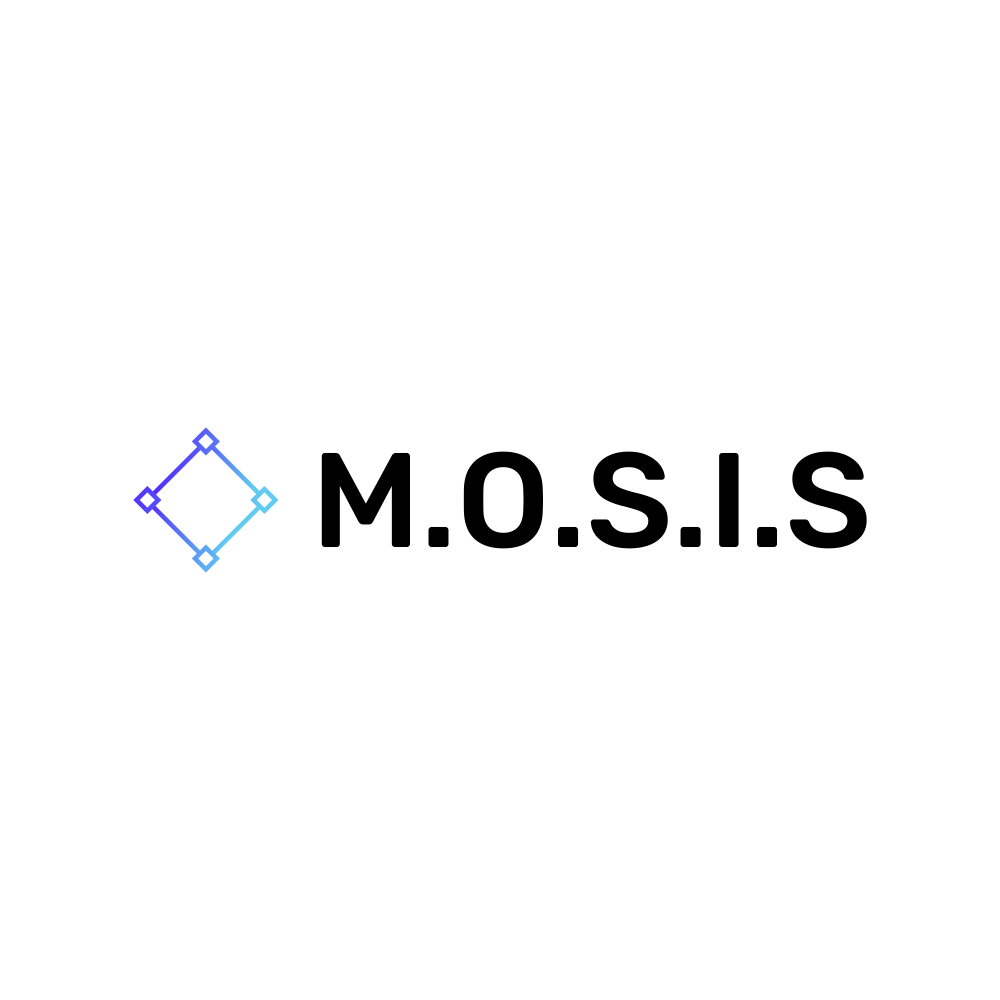
\includegraphics[scale=0.2]{../Title_Page/default.png}\\
    \Huge{\underline{M.O.S.I.S Host Software}\\}
    \Huge{\underline{User Guide}\\}
    \vspace{5cm}
    \large by\\
    Fabio J. Matos Nieves\\
    \normalsize
  \end{center}
\end{titlepage}

\tableofcontents
\newpage
\section{Installation}
\subsection{Windows}
\newpage
\begin{center}

	\begin{enumerate}
		\item Open a web browser
		      \begin{figure}[H]
			      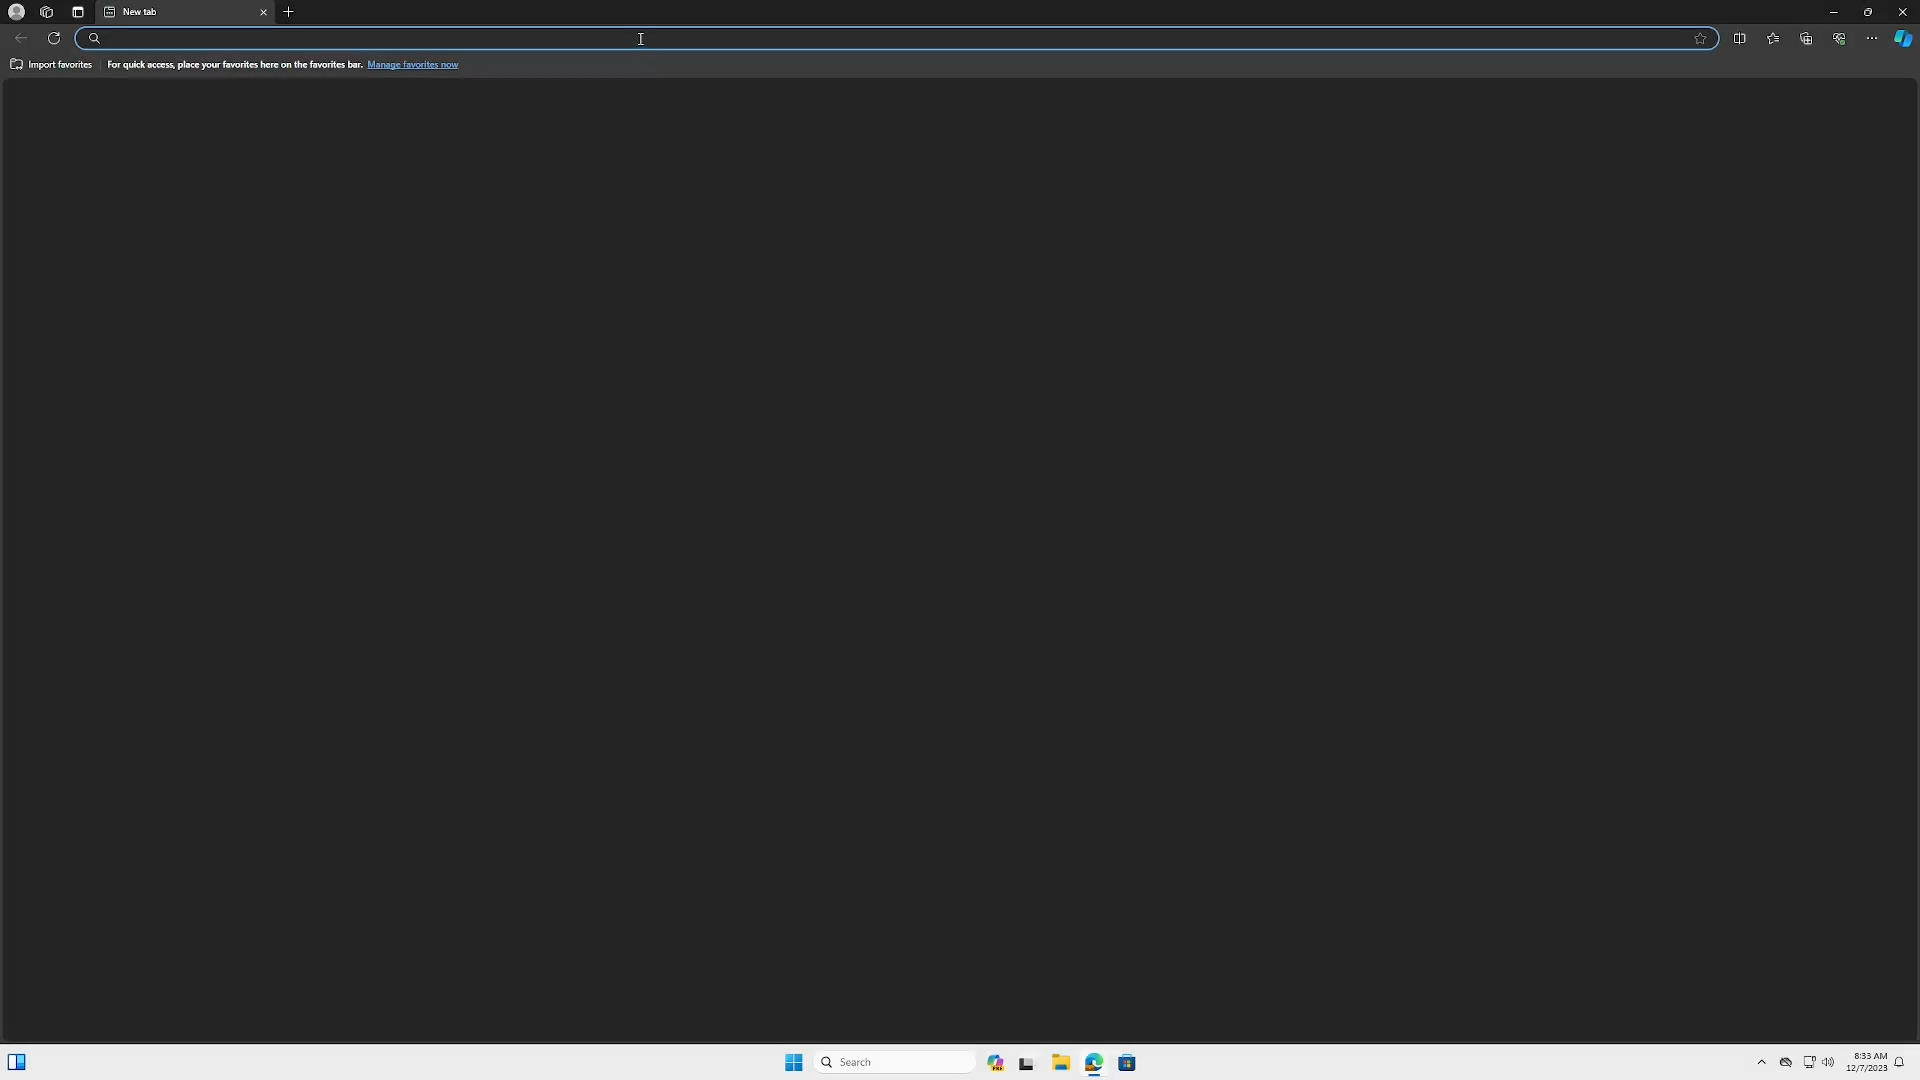
\includegraphics[width=\textwidth]{Figures/Windows-Open-Web-Browser.png}
		      \end{figure}
		\item Go to the repository going to \href{https://github.com/fabiomatos999/M.O.S.I.S}{https://github.com/fabiomatos999/M.O.S.I.S} by clicking here: \href{https://github.com/fabiomatos999/M.O.S.I.S}{link}.
		      \begin{figure}[H]
			      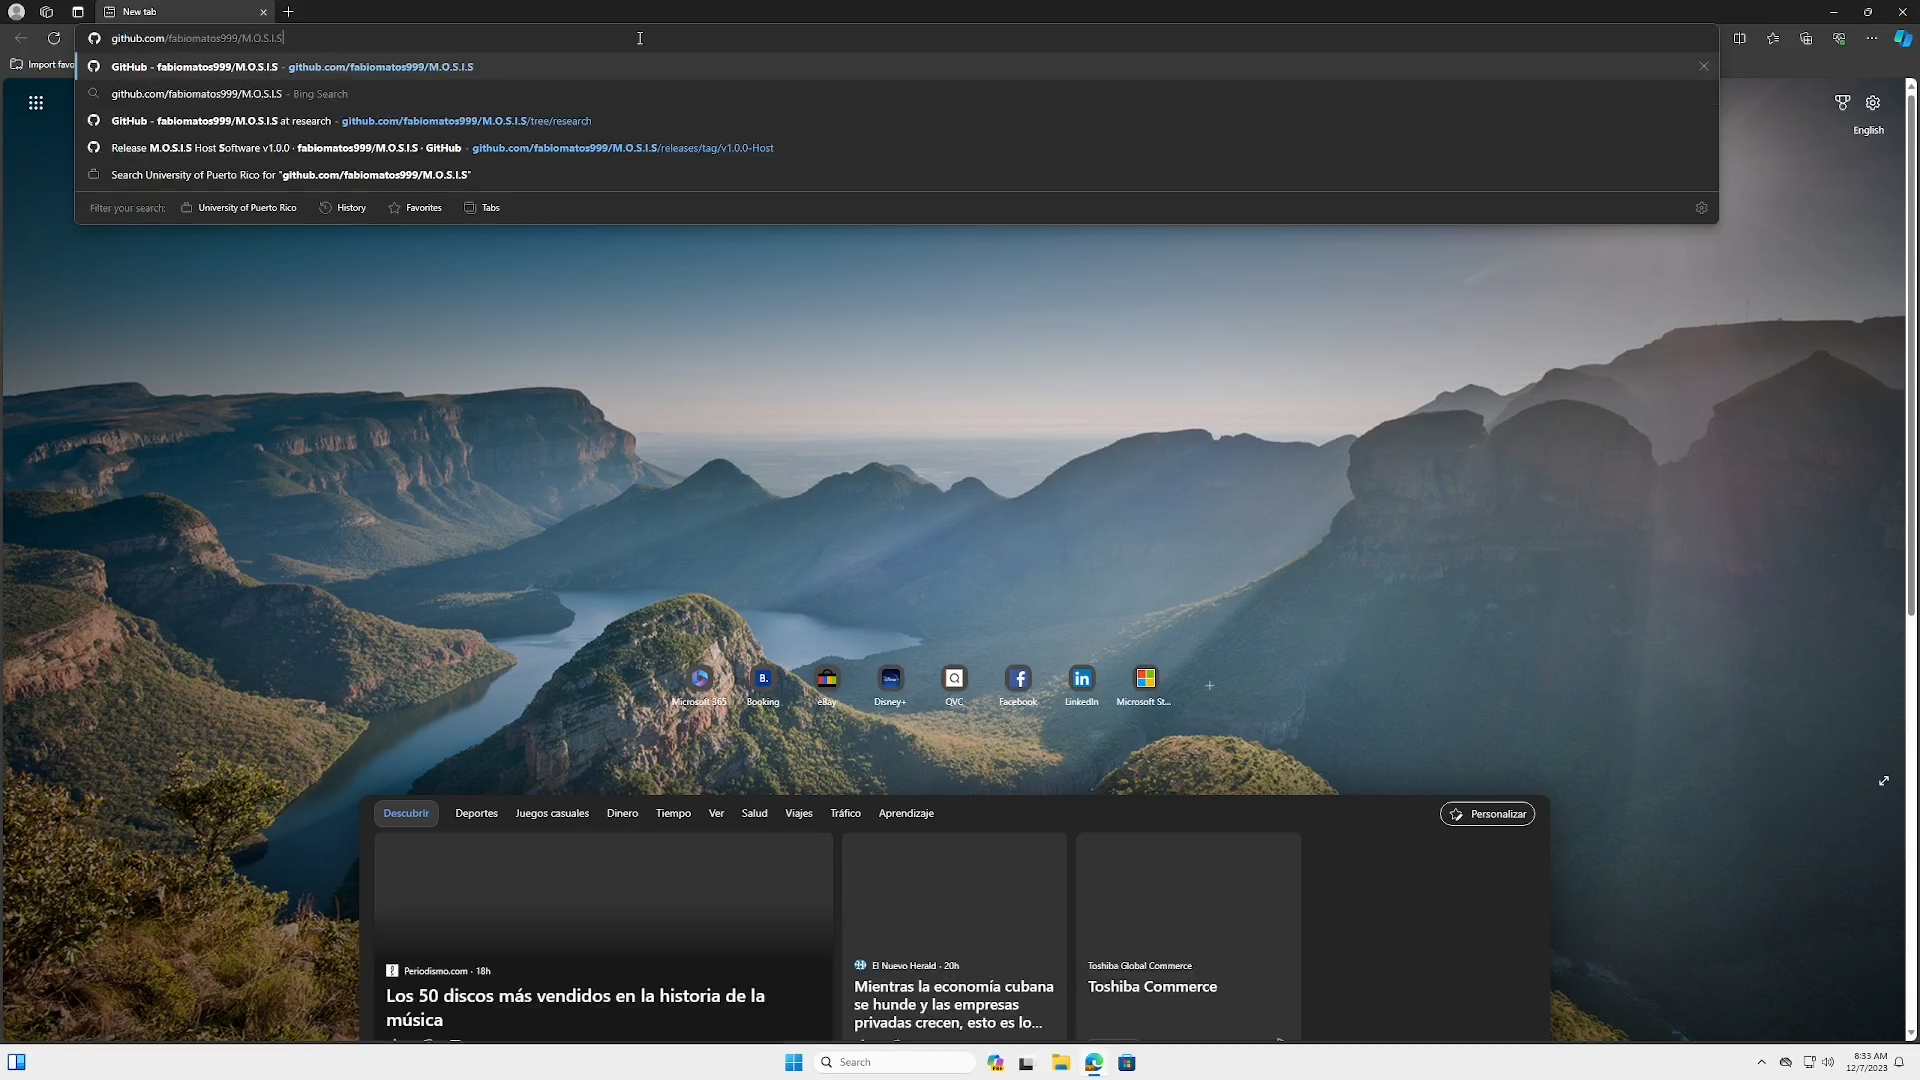
\includegraphics[width=\textwidth]{Figures/Windows-Go-To-Repo.png}
		      \end{figure}
		\item Go the releases page on the Github repository:
		      \begin{figure}[H]
			      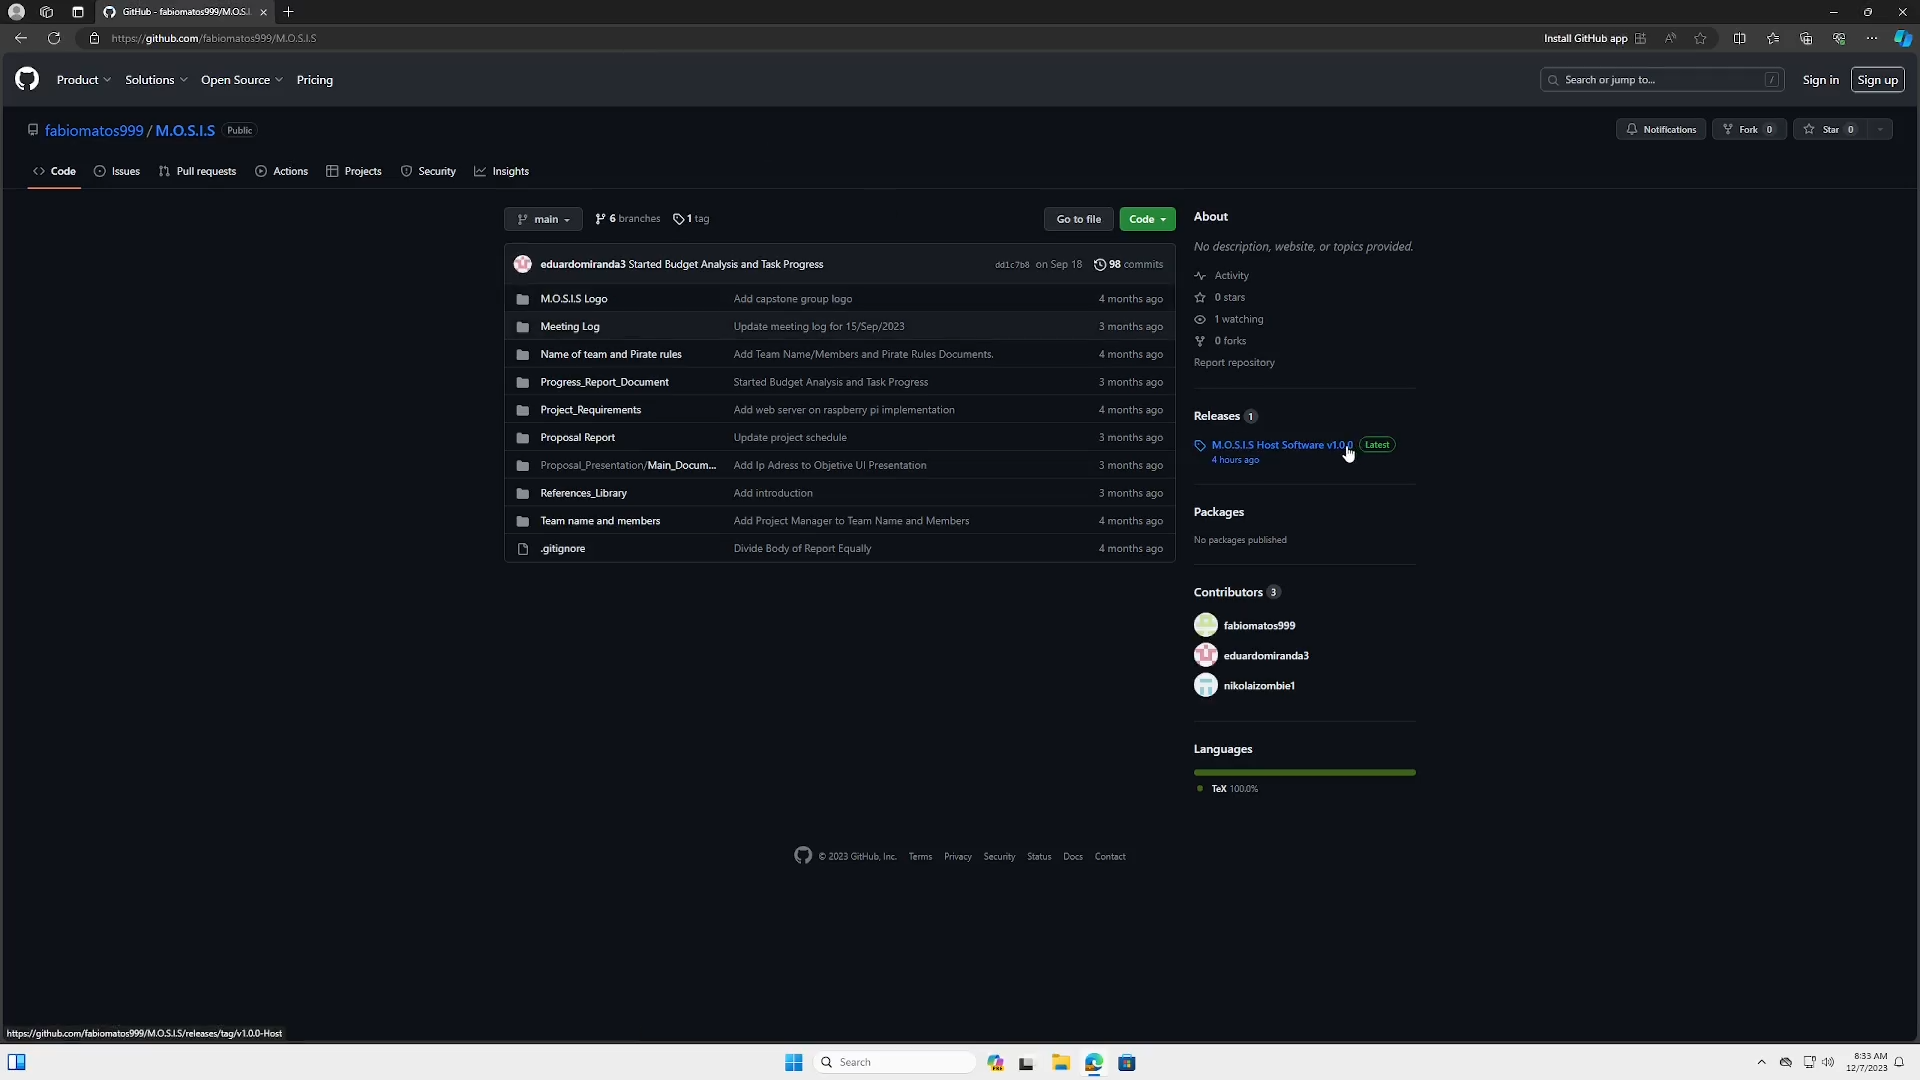
\includegraphics[width=\textwidth]{Figures/Windows-Go-To-Releases.png}
		      \end{figure}
		\item Get Host Software by clicking on the ``M.O.S.I.S\_Host\_Software.zip'' in the latest release (at the time writing v1.0.0)
		      \begin{figure}[H]
			      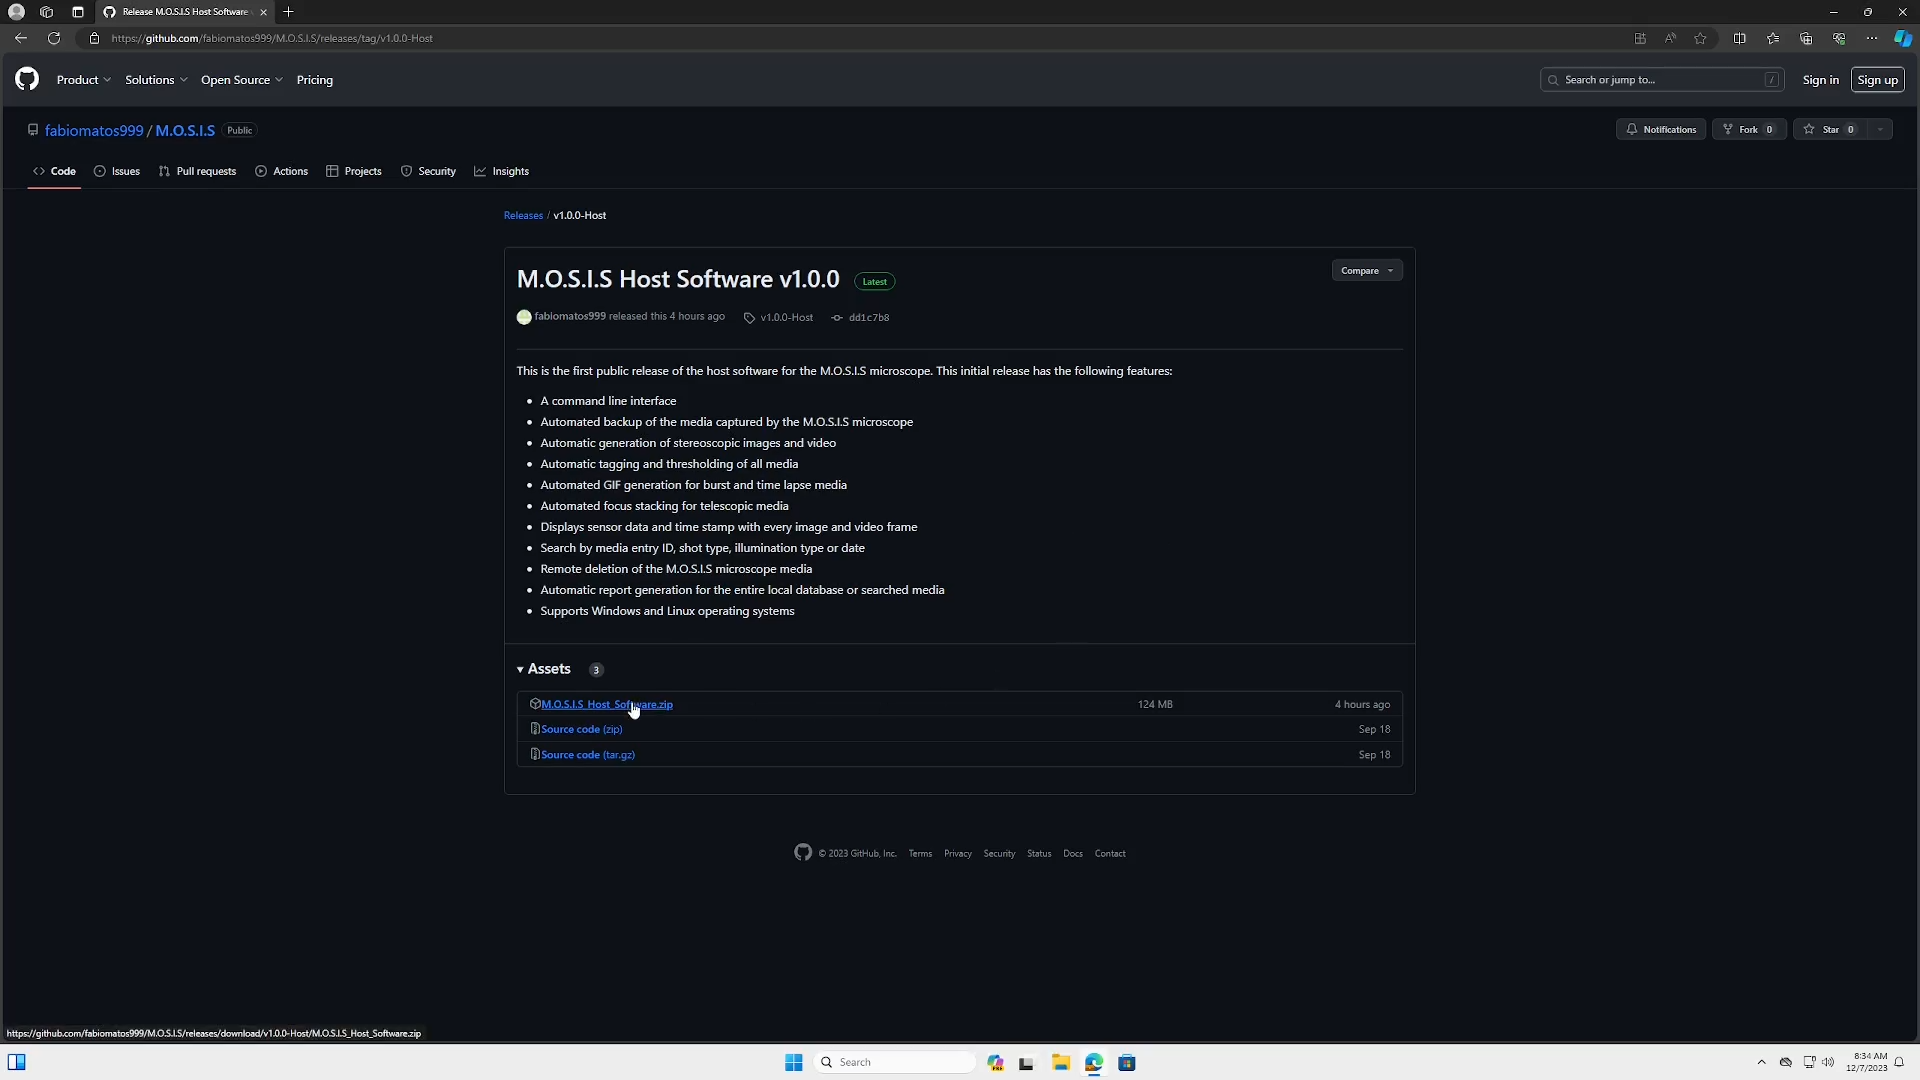
\includegraphics[width=\textwidth]{Figures/Windows-Get-Host-Software.png}
		      \end{figure}
		\item When the ``zip'' file has finished downloading, go to where the file downloaded (in most cases should be the Downloads folder), right click it and select extract all.
		      \begin{figure}[H]
			      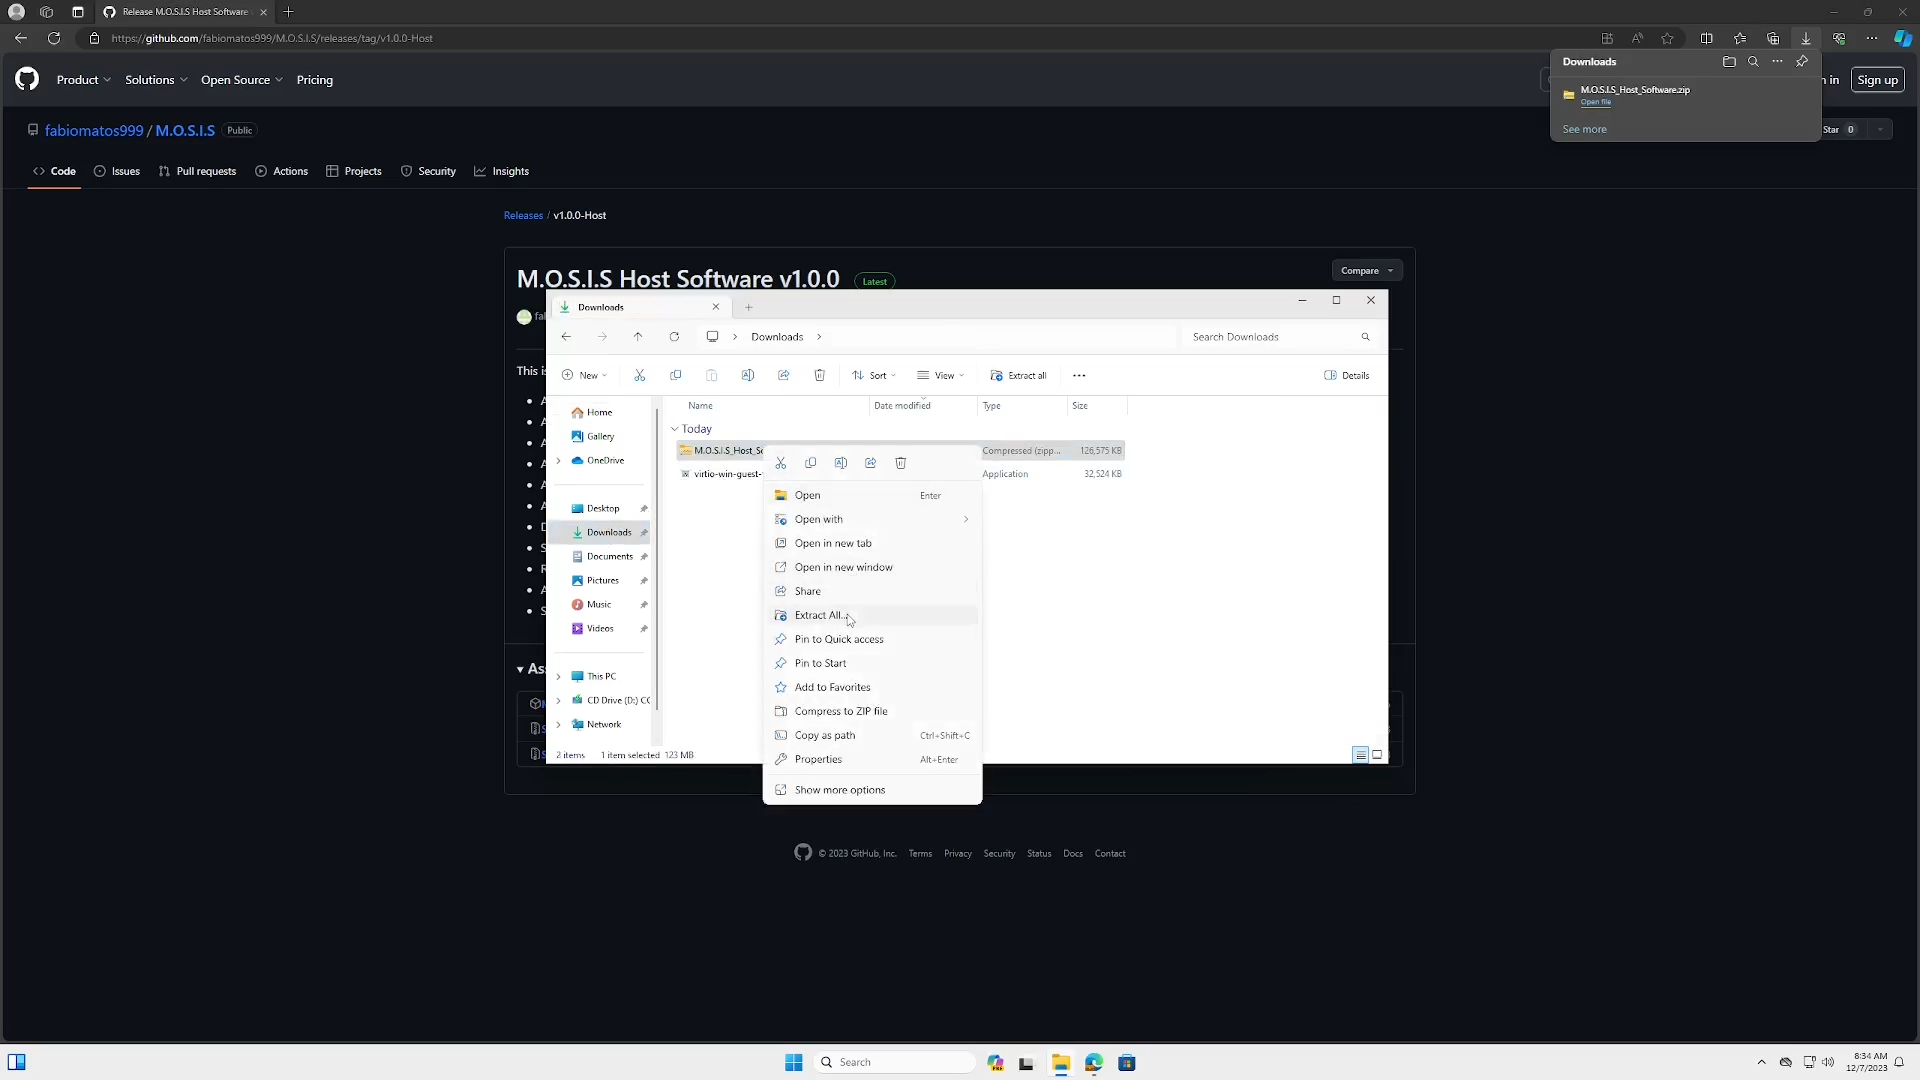
\includegraphics[width=\textwidth]{Figures/Windows-Extract-Archive.png}
		      \end{figure}
		\item A menu should pop up prompting you to chose where you want to extract the file, click next if you want to extract it in the downloads folder
		      \begin{figure}[H]
			      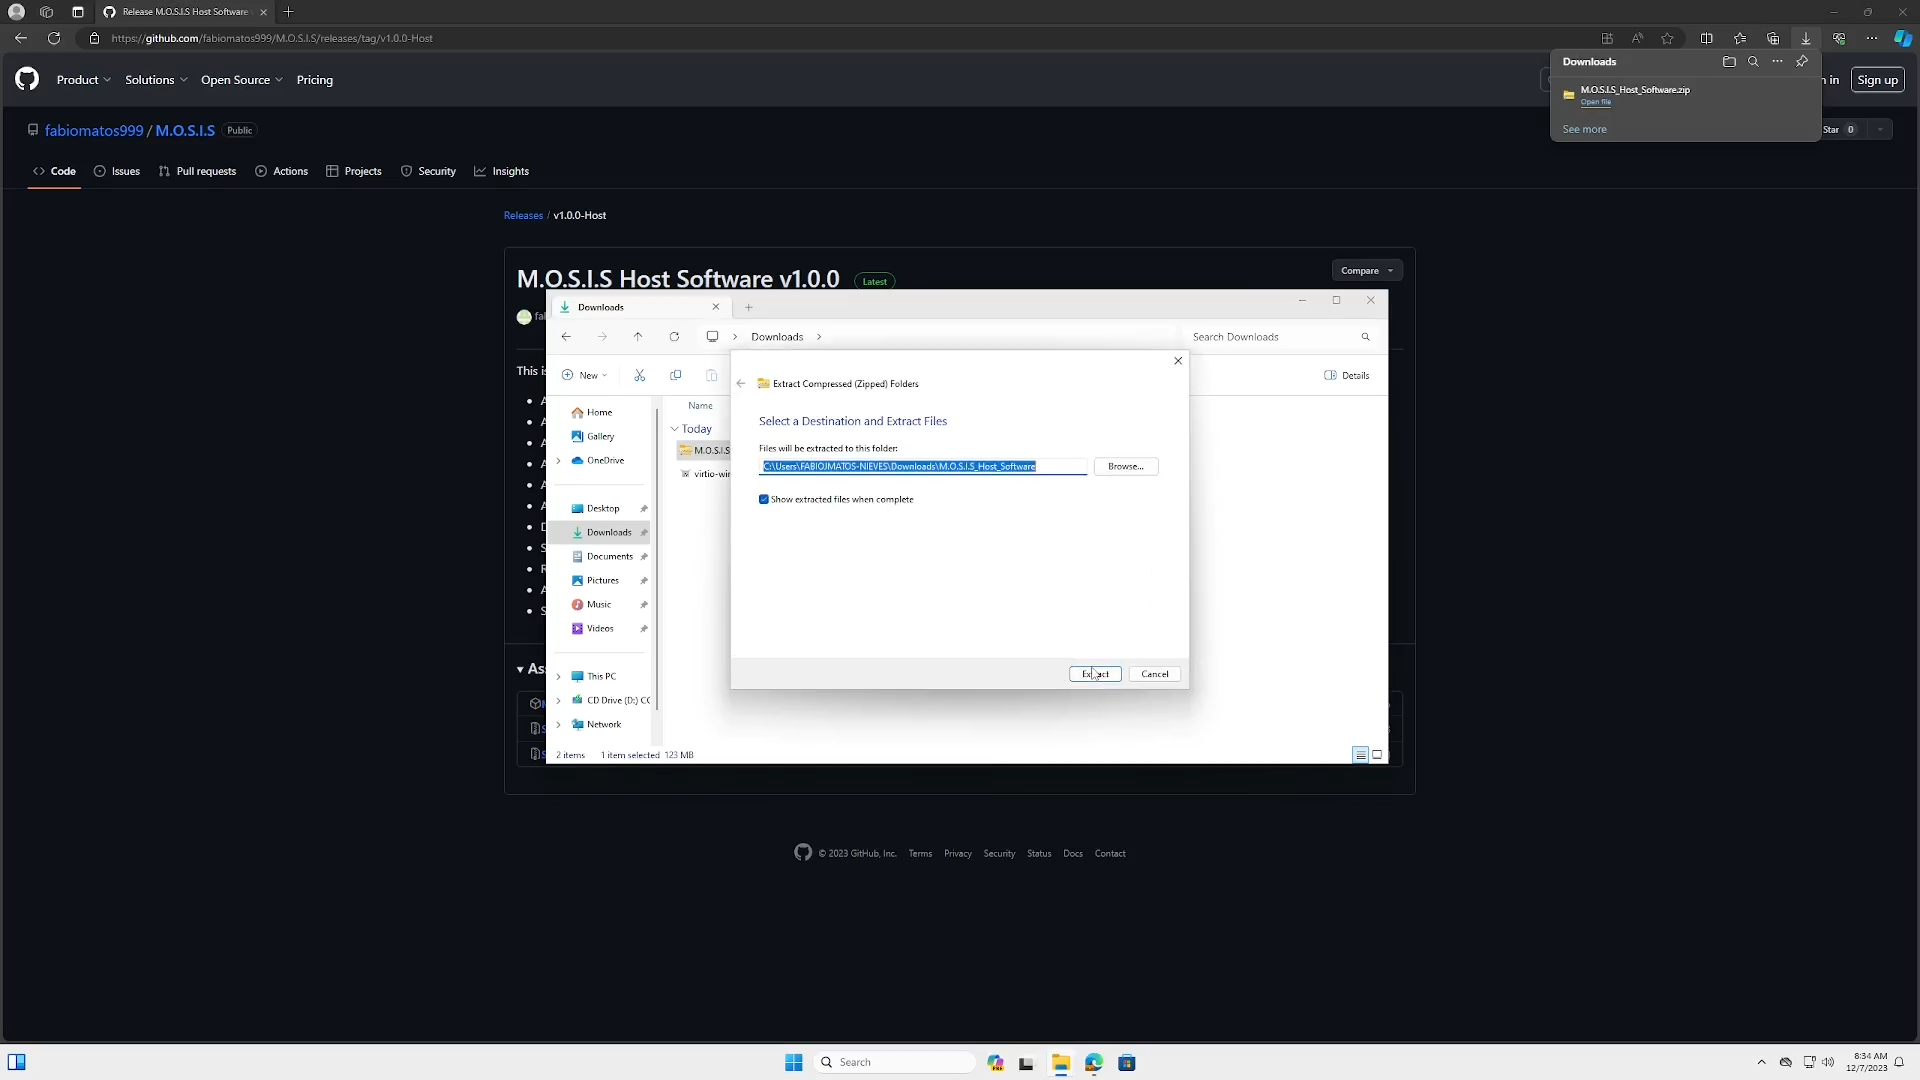
\includegraphics[width=\textwidth]{Figures/Windows-Extract-Archive-Menu.png}
		      \end{figure}
		\item Once the archive has been extracted, click on the search bar at the bottom of the screen and search ``Powershell''. To the right of the top most search result, a series of options should appear, click on the ``Run as the administrator''
		      \begin{figure}[H]
			      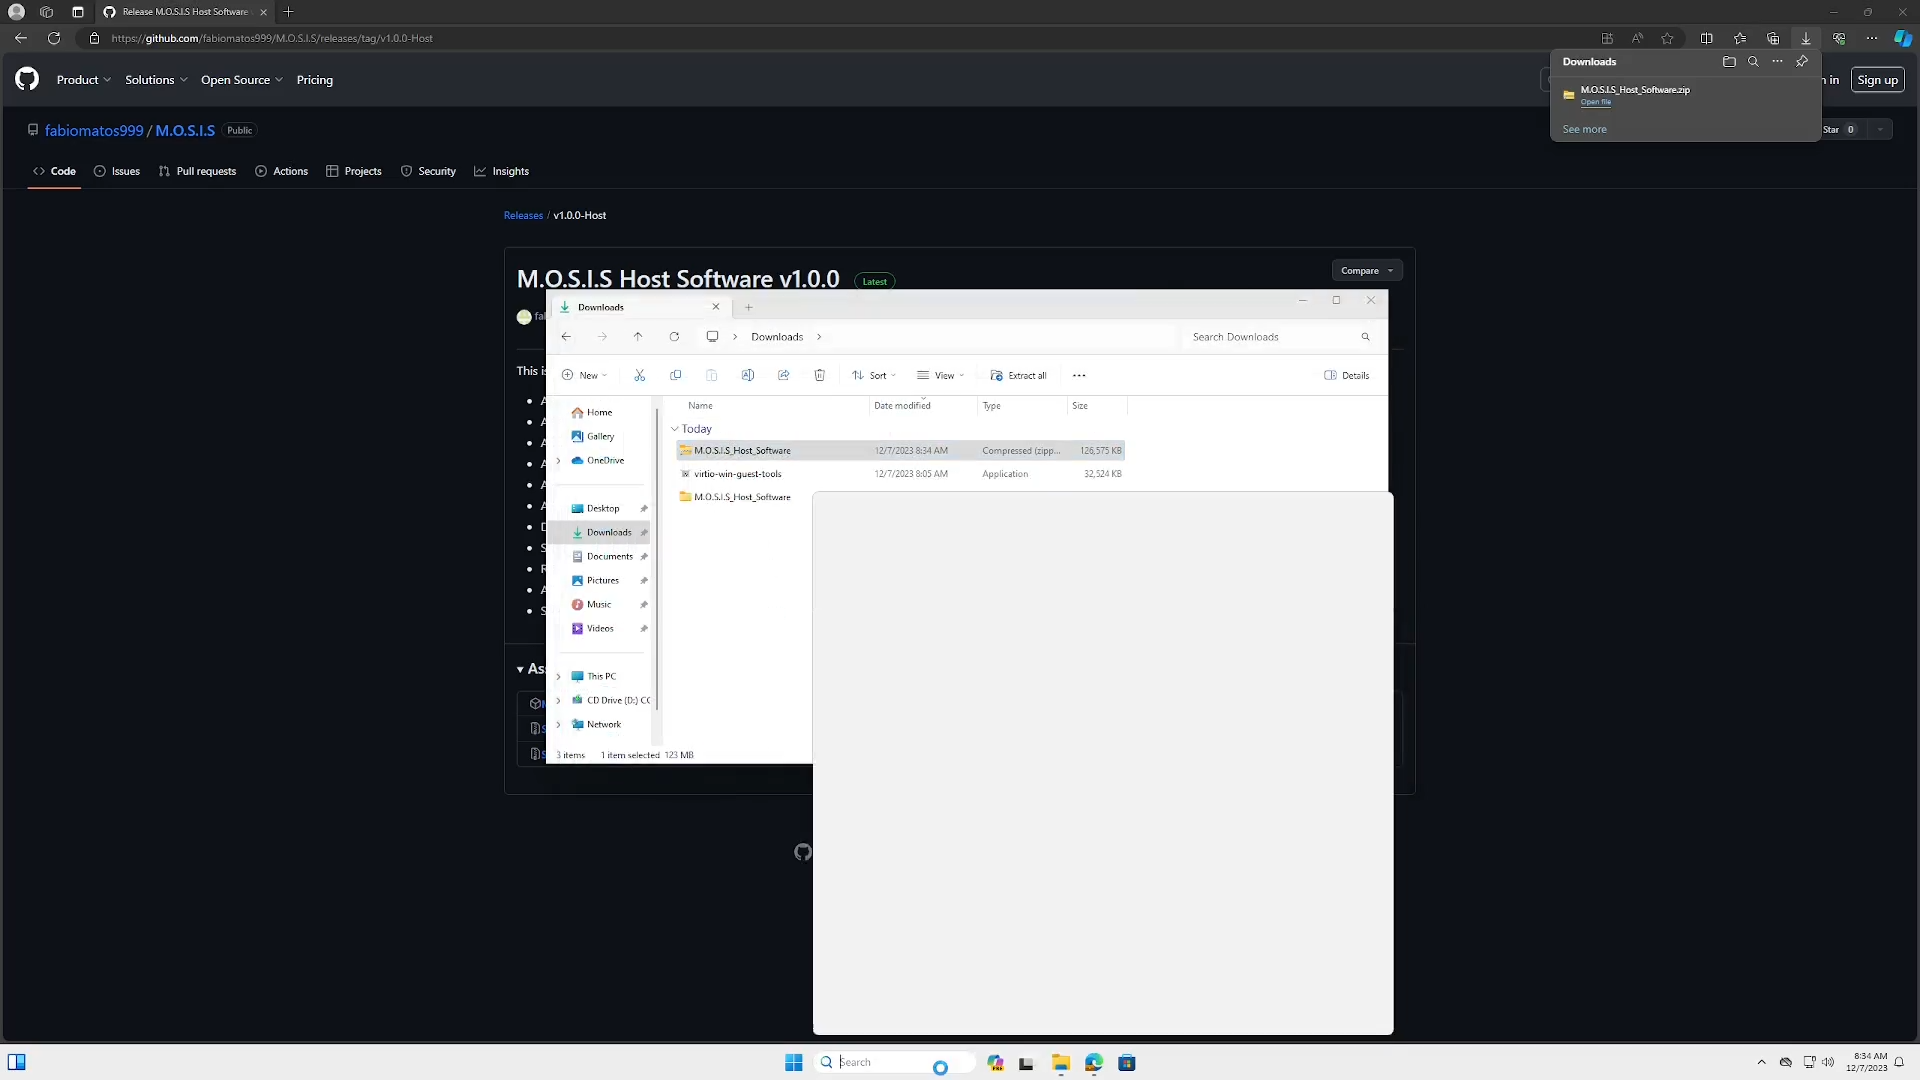
\includegraphics[width=\textwidth]{Figures/Windows-Open-Search.png}
		      \end{figure}
		      \begin{figure}[H]
			      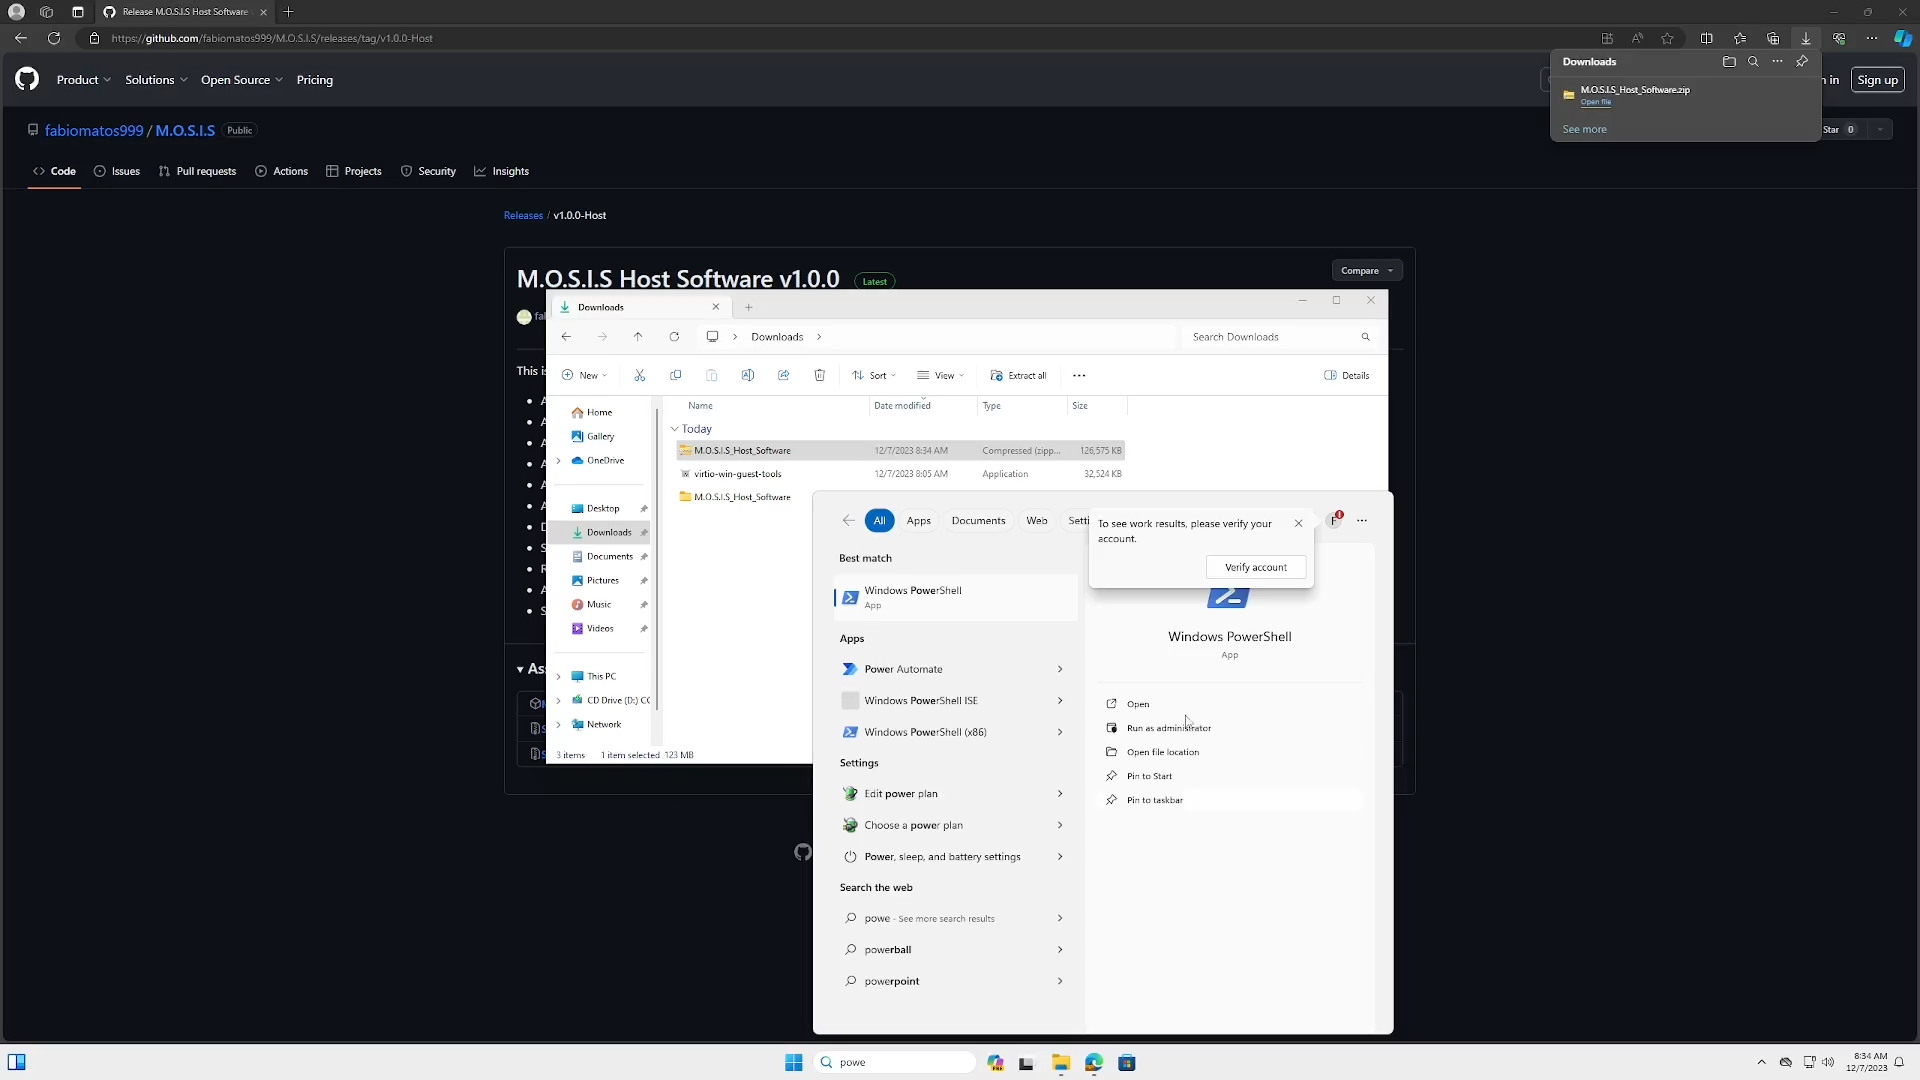
\includegraphics[width=\textwidth]{Figures/Windows-Open-Powershell-As-Admin.png}
		      \end{figure}
		\item If prompted by the following screen, click yes.
		      \begin{figure}[H]
			      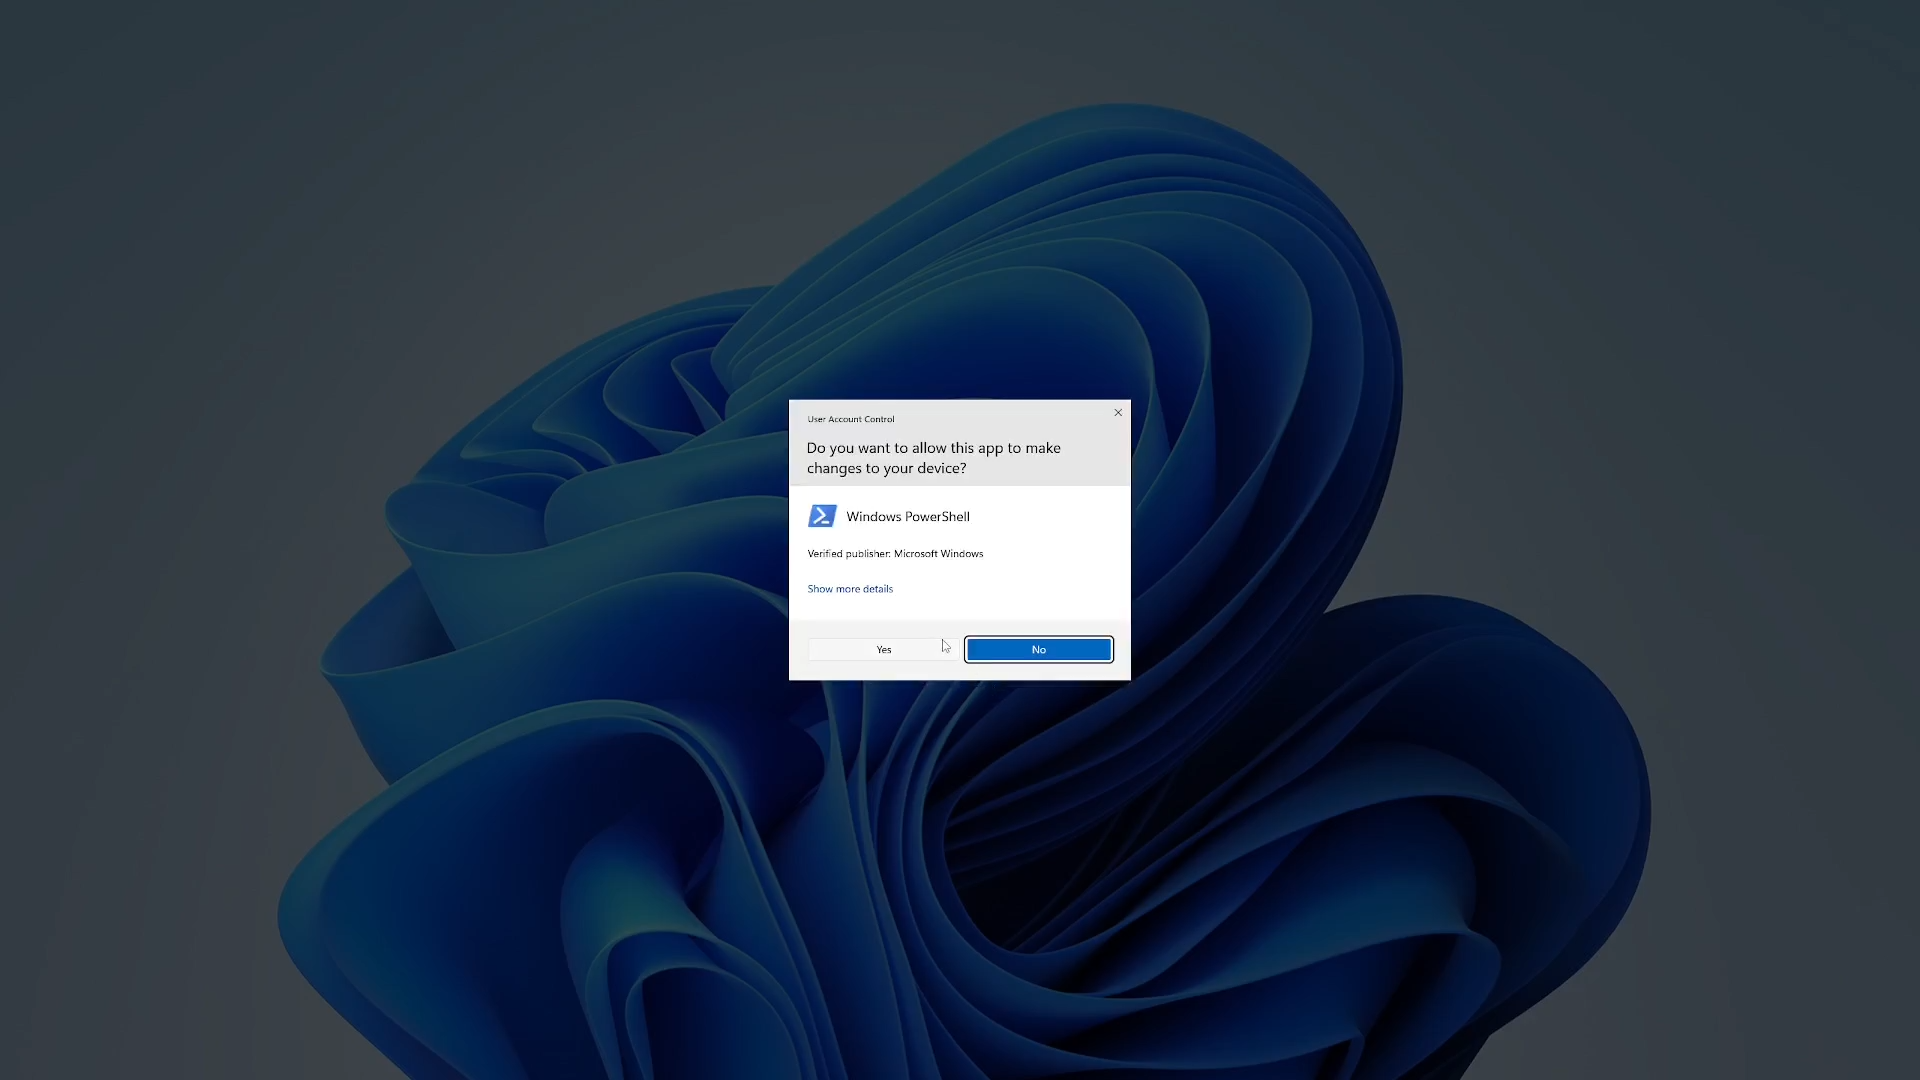
\includegraphics[width=\textwidth]{Figures/Windows-UAC-Prompt.png}
		      \end{figure}
		\item Once the Powershell has opened, type the following command and then press enter
		      \begin{minted}{ps1}
    Set-ExecutionPolicy unrestricted
  \end{minted}
		      \begin{figure}[H]
			      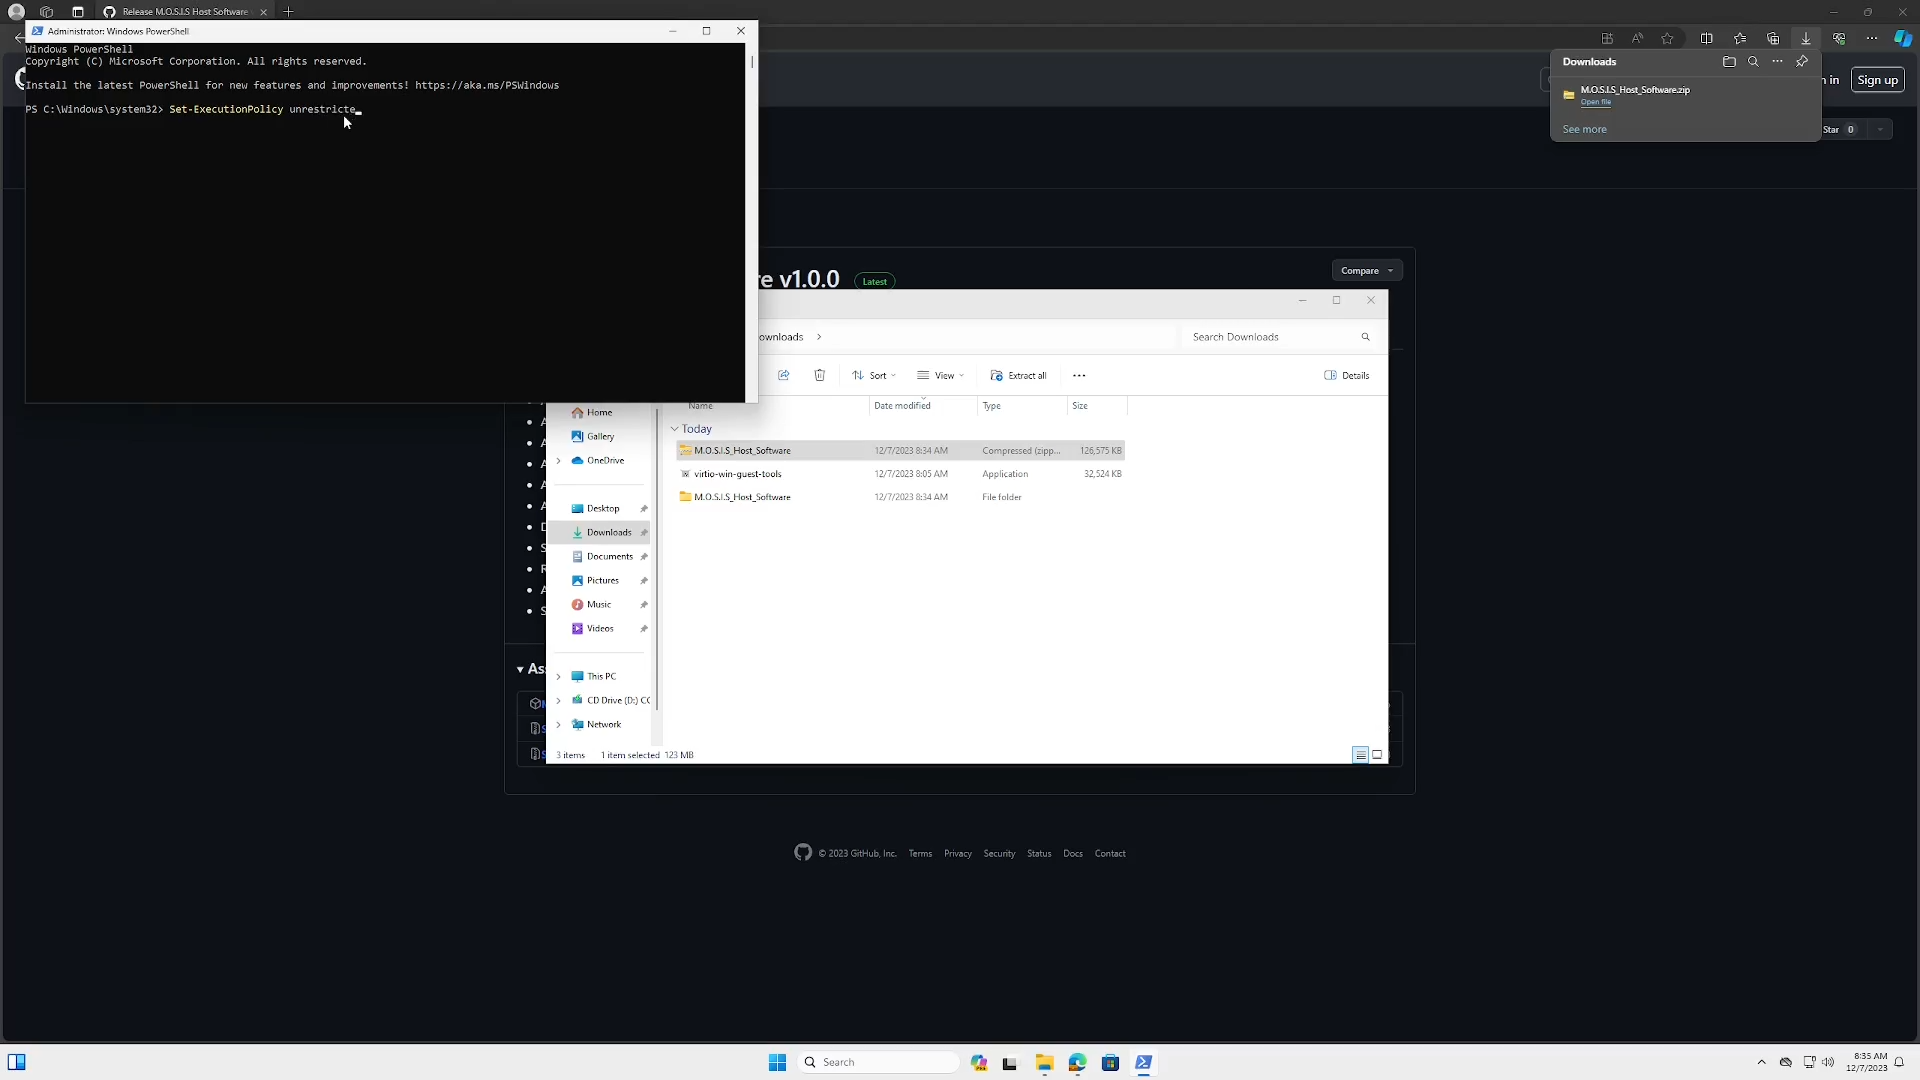
\includegraphics[width=\textwidth]{Figures/Windows-Set-ExecutionPolicy-unrestricted.png}
		      \end{figure}
		\item If prompted to confirm the changes, type ``y'' and press enter
		      \begin{figure}[H]
			      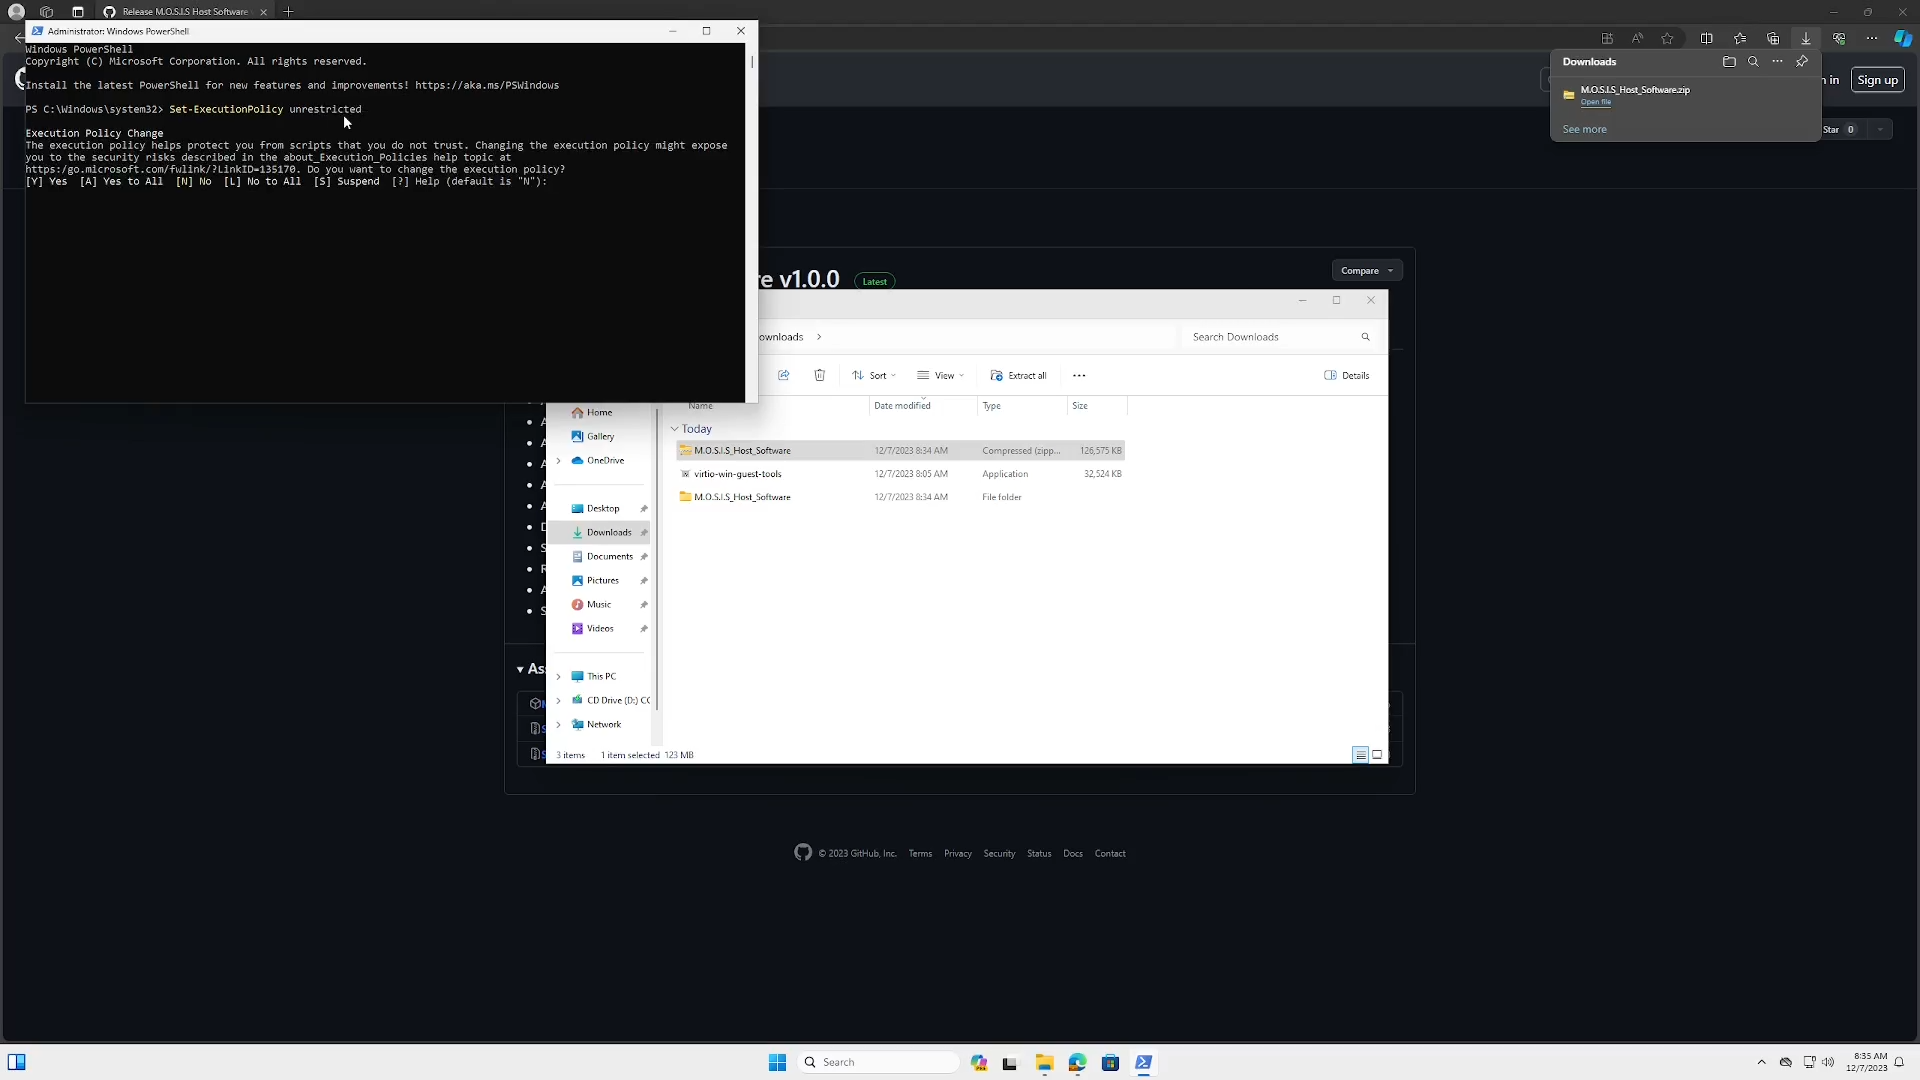
\includegraphics[width=\textwidth]{Figures/Windows-Set-ExecutionPolicy-Confim.png}
		      \end{figure}
		\item Close the Powershell by clicking on the X on the top right corner and open Powershell again, but click on the ``open'' button
		      \begin{figure}[H]
			      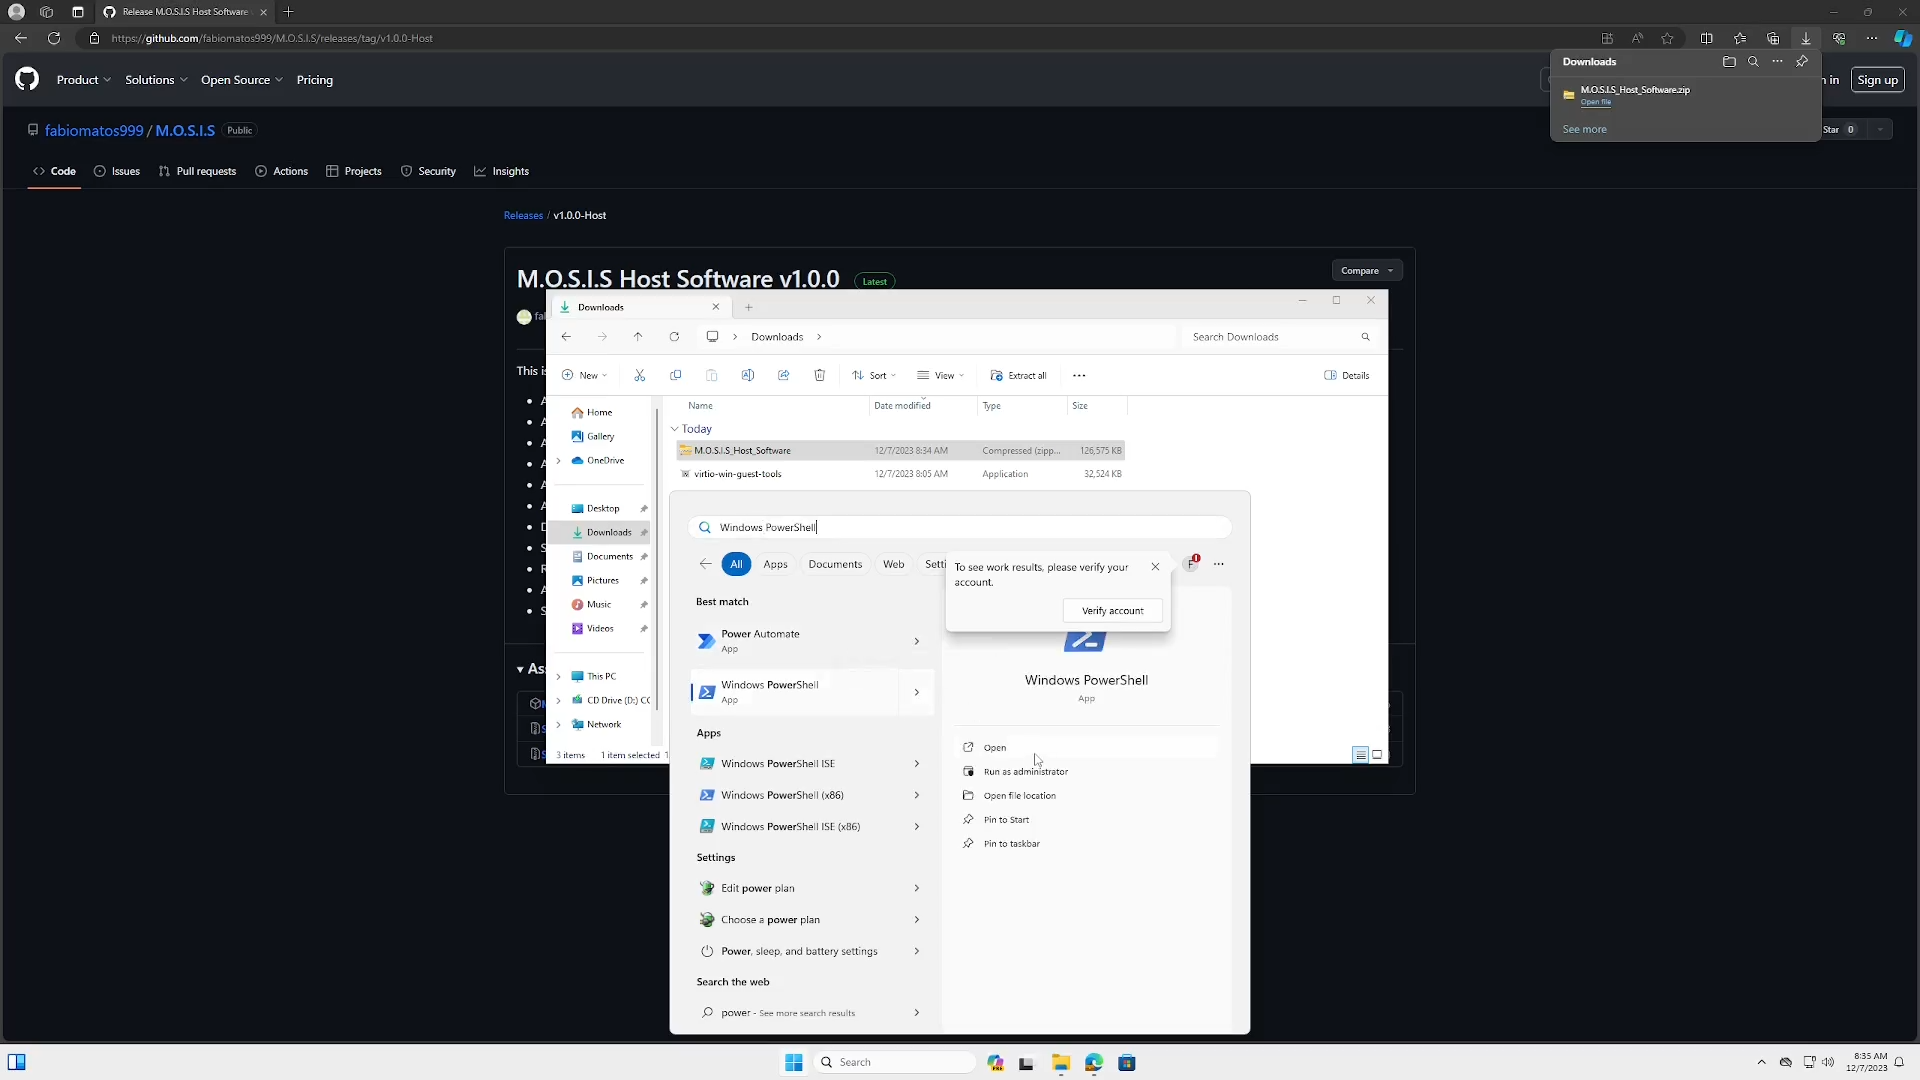
\includegraphics[width=\textwidth]{Figures/Windows-Open-Powershell.png}
		      \end{figure}
		\item Now change directory into where you extracted the host software. Assuming you extracted the host software zip in the Downloads folder, type the following command into the Powershell and press enter.
		      \small\begin{minted}[breaksymbolleft=]{ps1}
    cd .\Downloads\M.O.S.I.S_Host_Software\M.O.S.I.S_Host_Software\App\
  \end{minted}
		      \normalsize
		      \begin{figure}[H]
			      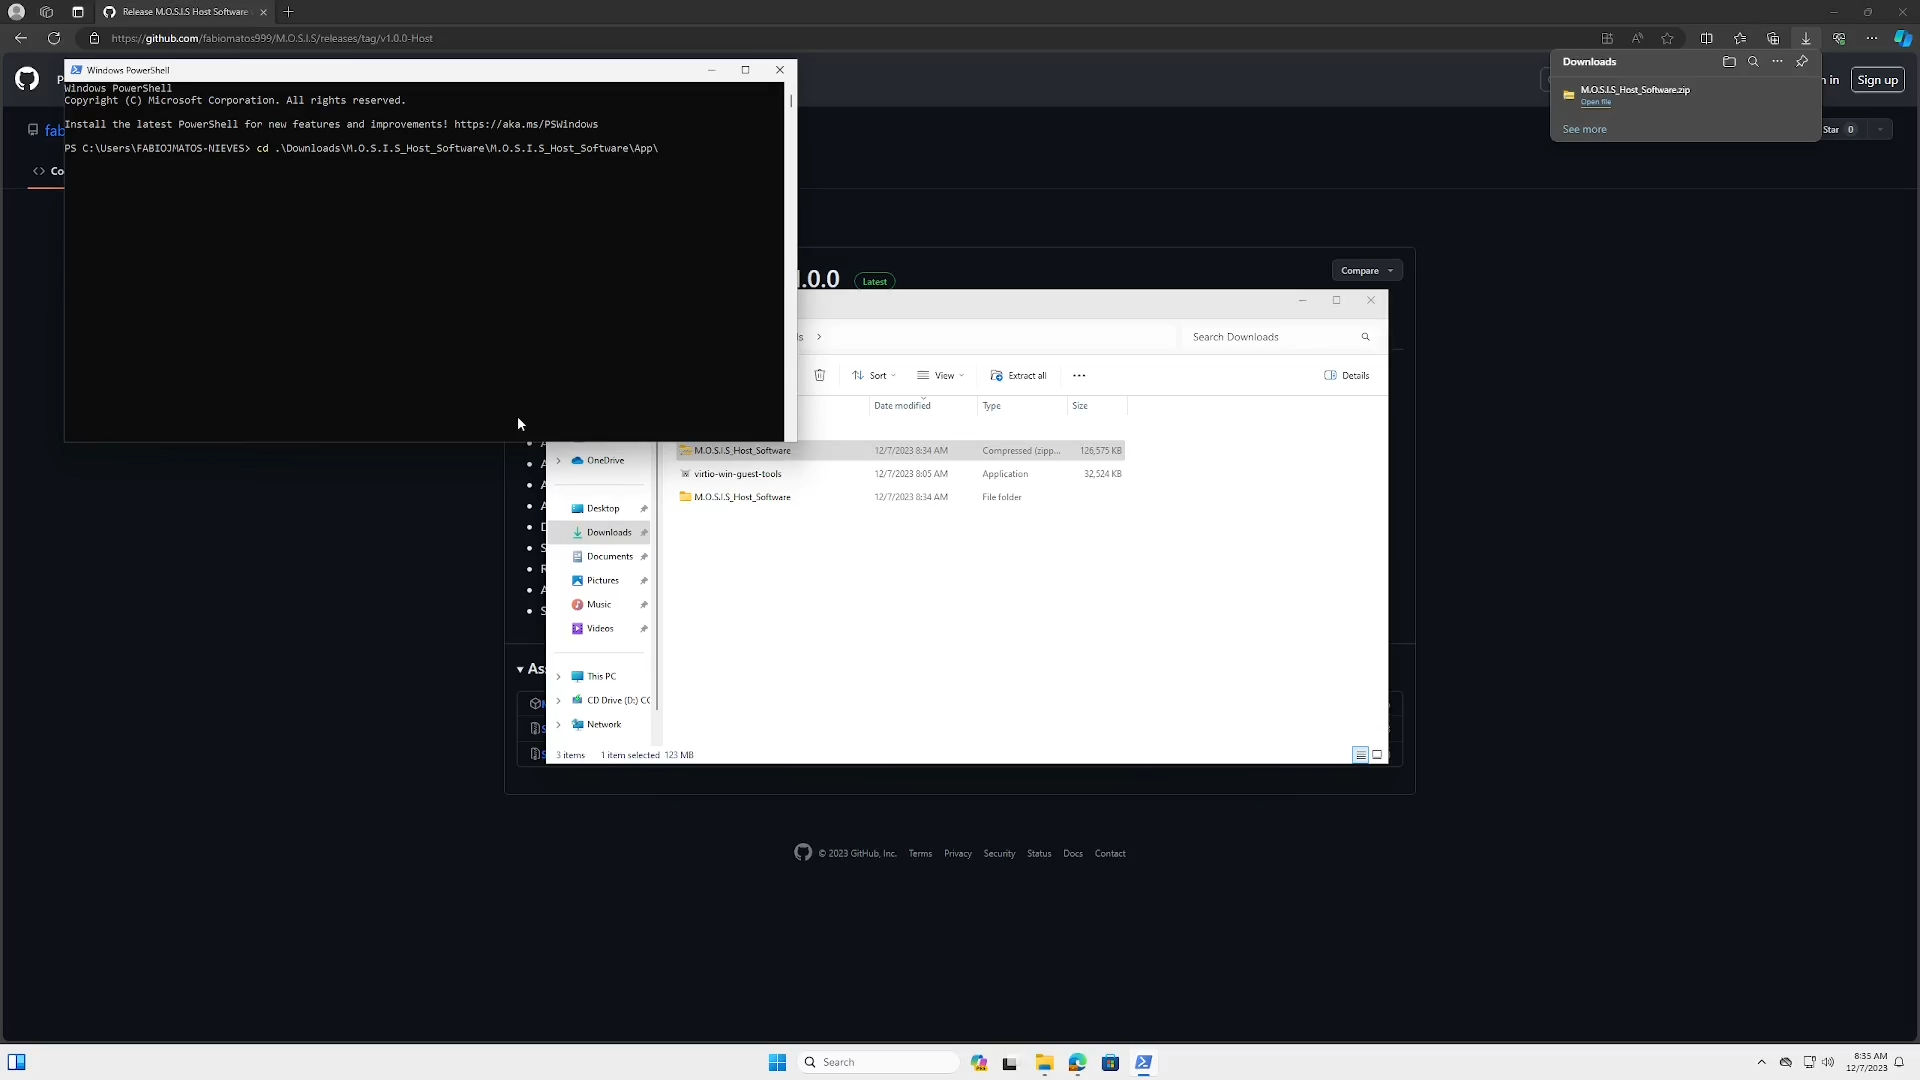
\includegraphics[width=\textwidth]{Figures/Windows-cd-Into-Host-Software.png}
		      \end{figure}
		\item Start the host software for the first time by inputting the following command into the Powershell and press enter.
		      \begin{minted}{ps1}
    .\start_app.ps1 -n
  \end{minted}
		      \begin{figure}[H]
			      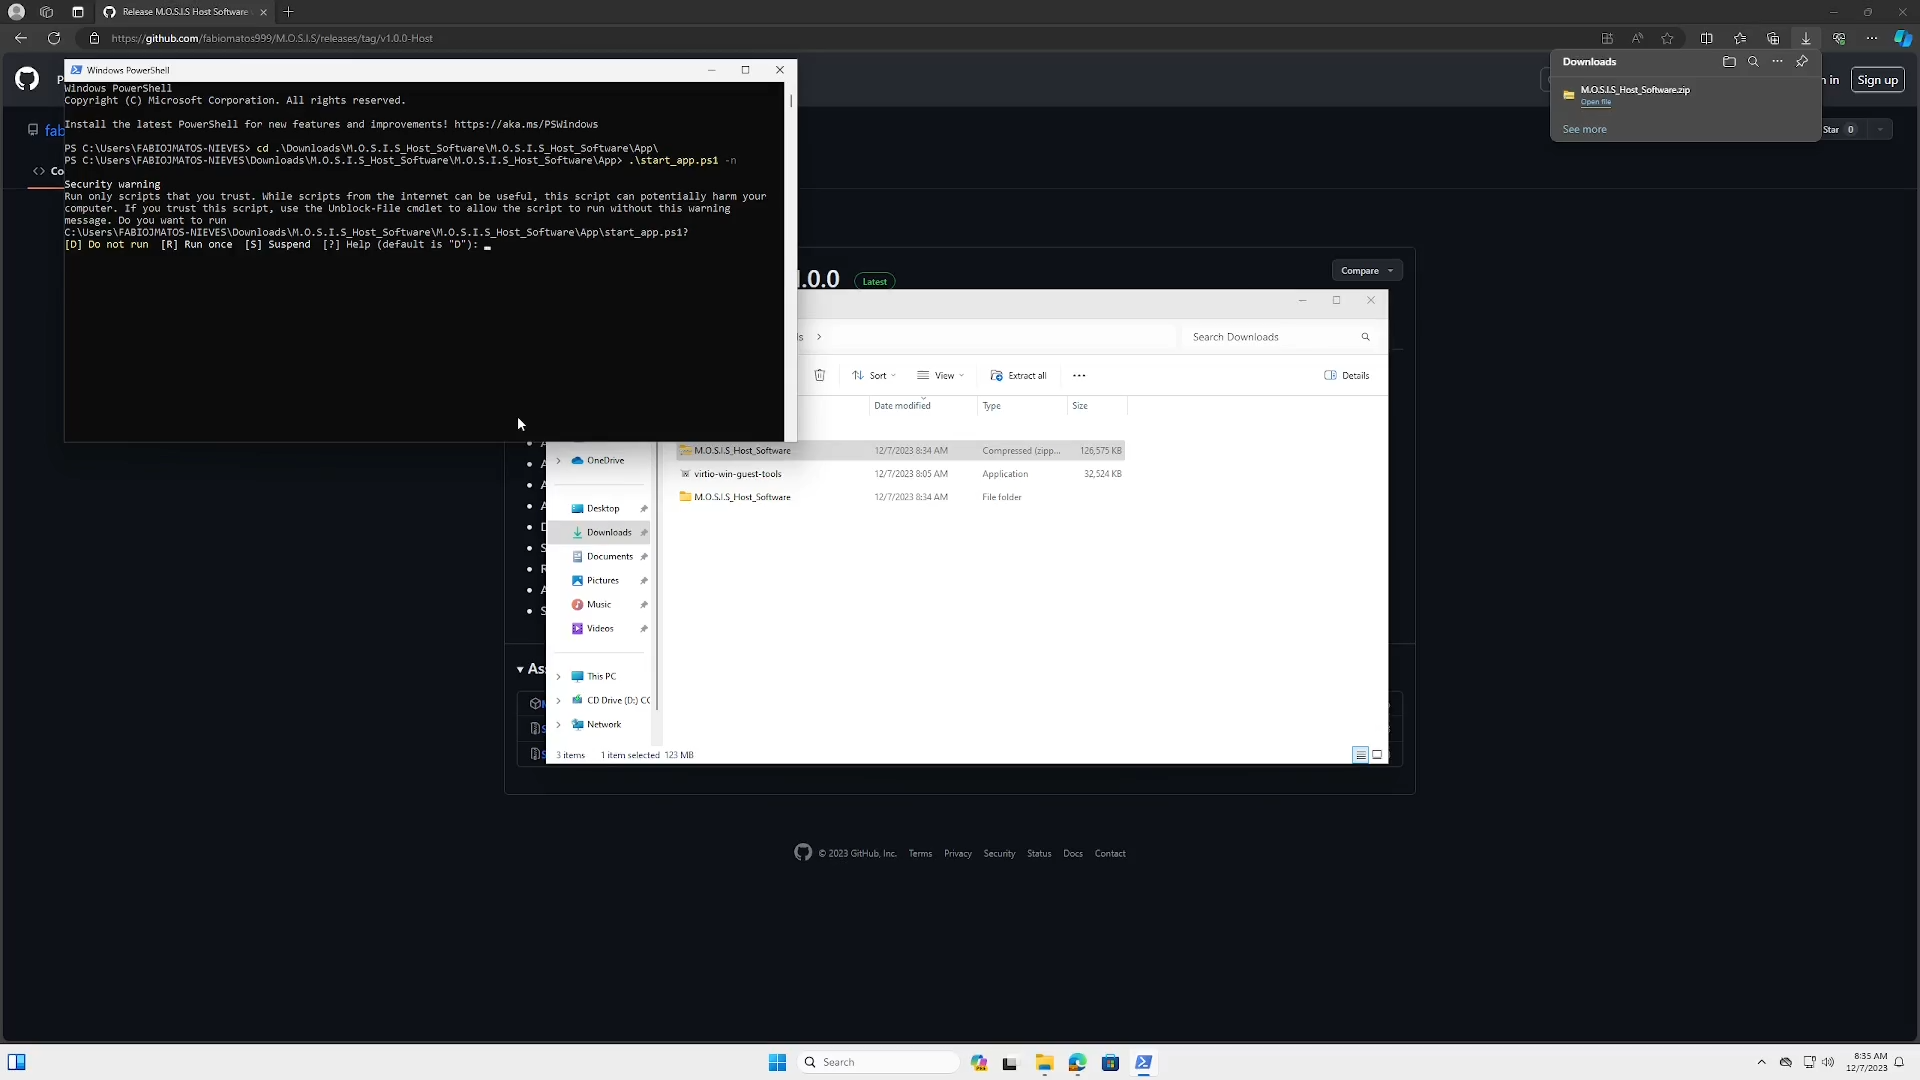
\includegraphics[width=\textwidth]{Figures/Windows-Host-Software-Confim-Run-Once.png}
		      \end{figure}
		\item If prompted by the following screen, click ``yes''
		      \begin{figure}[H]
			      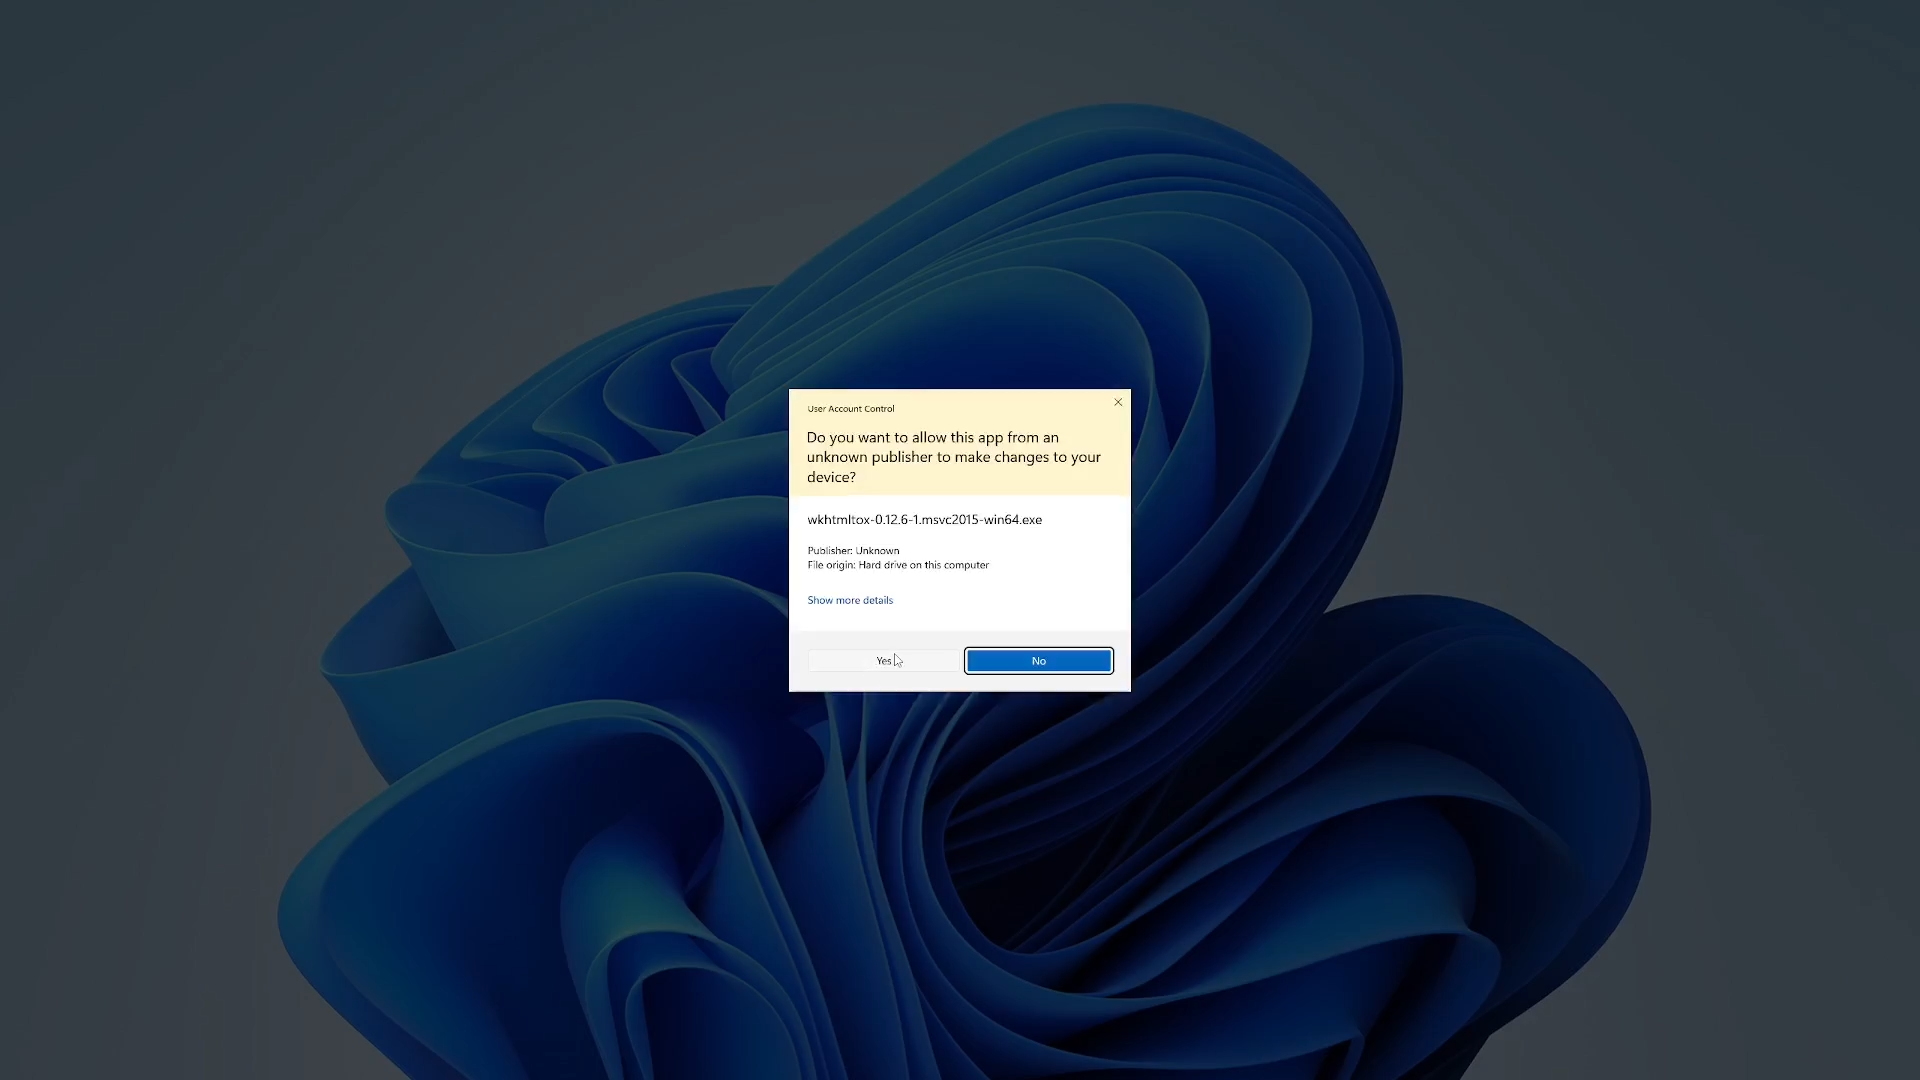
\includegraphics[width=\textwidth]{Figures/Windows-UAC-Pompt-wkhtmltopdf.png}
		      \end{figure}
		\item The following installer should appear on screen. Click on the ``I agree'' button.
		      \begin{figure}[H]
			      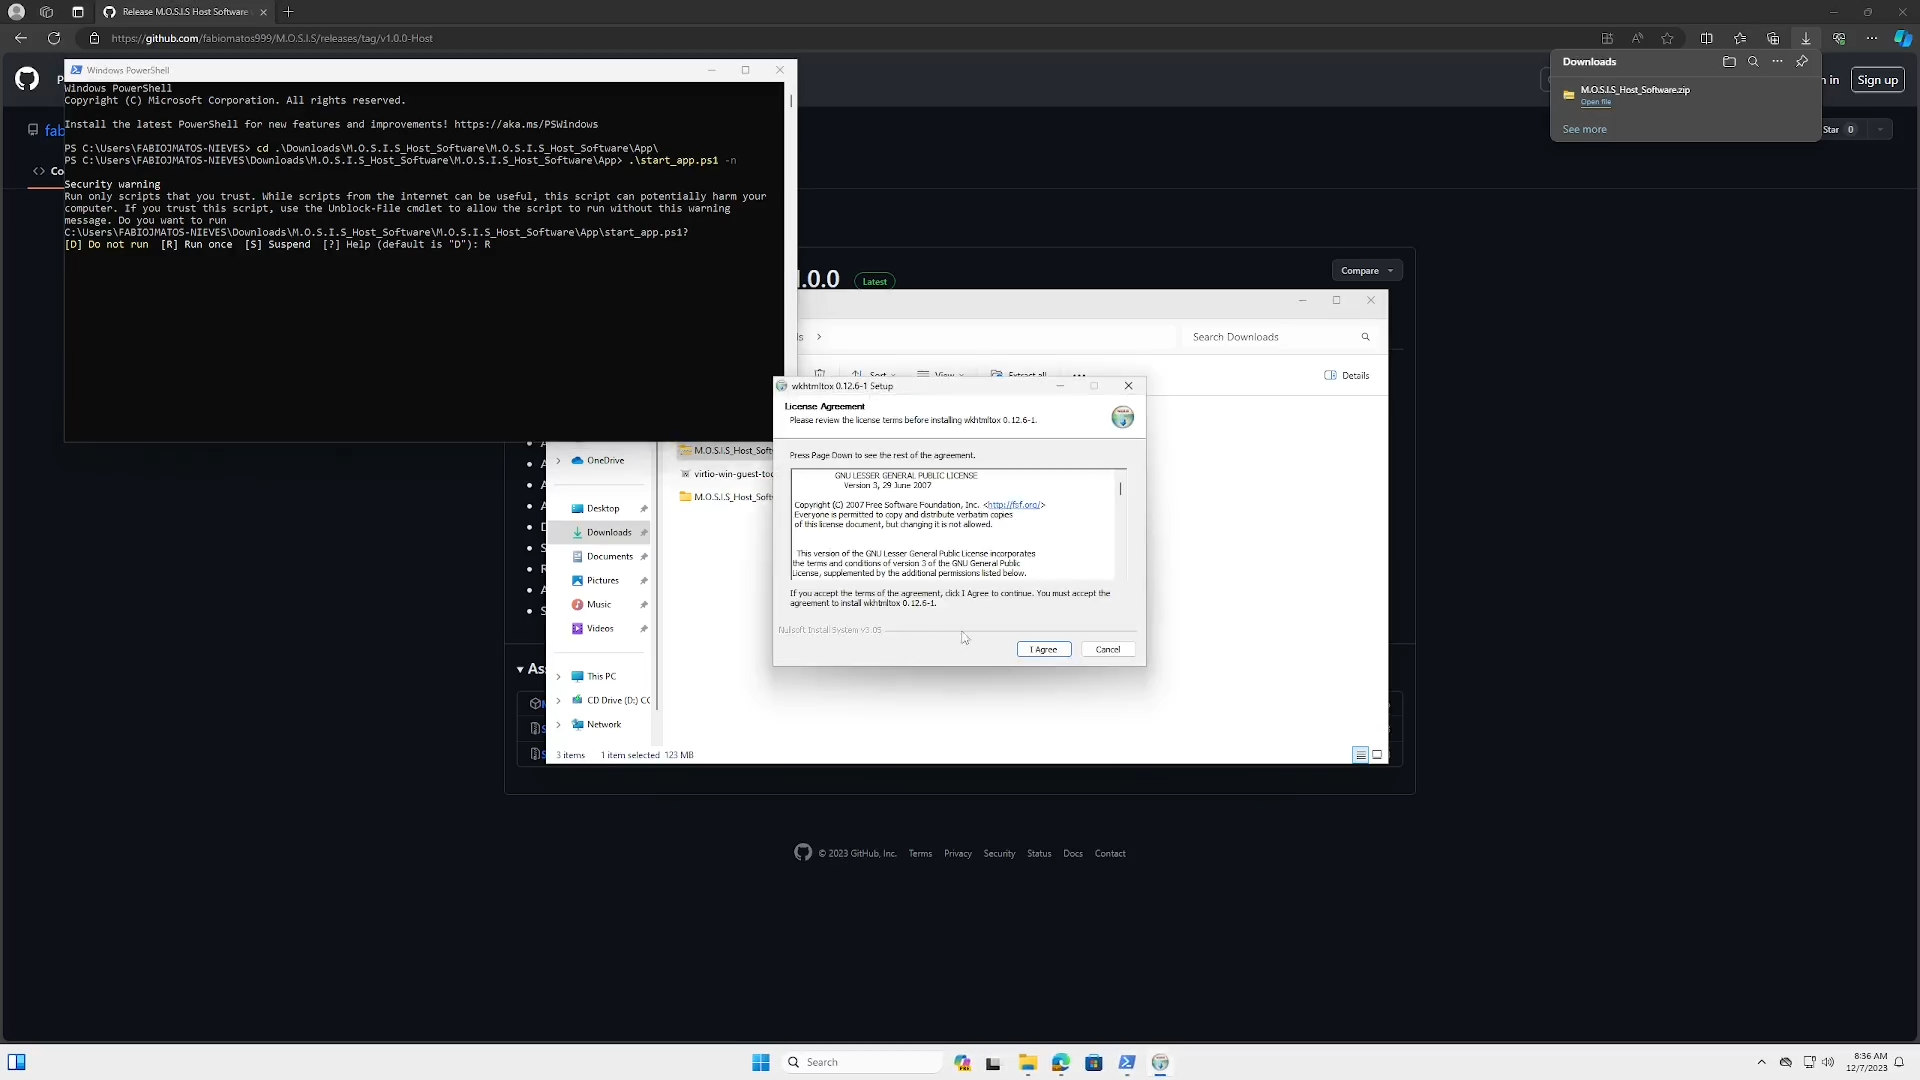
\includegraphics[width=\textwidth]{Figures/Windows-wkhtmltopdf-Menu-1.png}
		      \end{figure}
		\item Click on the ``Install'' button
		      \begin{figure}[H]
			      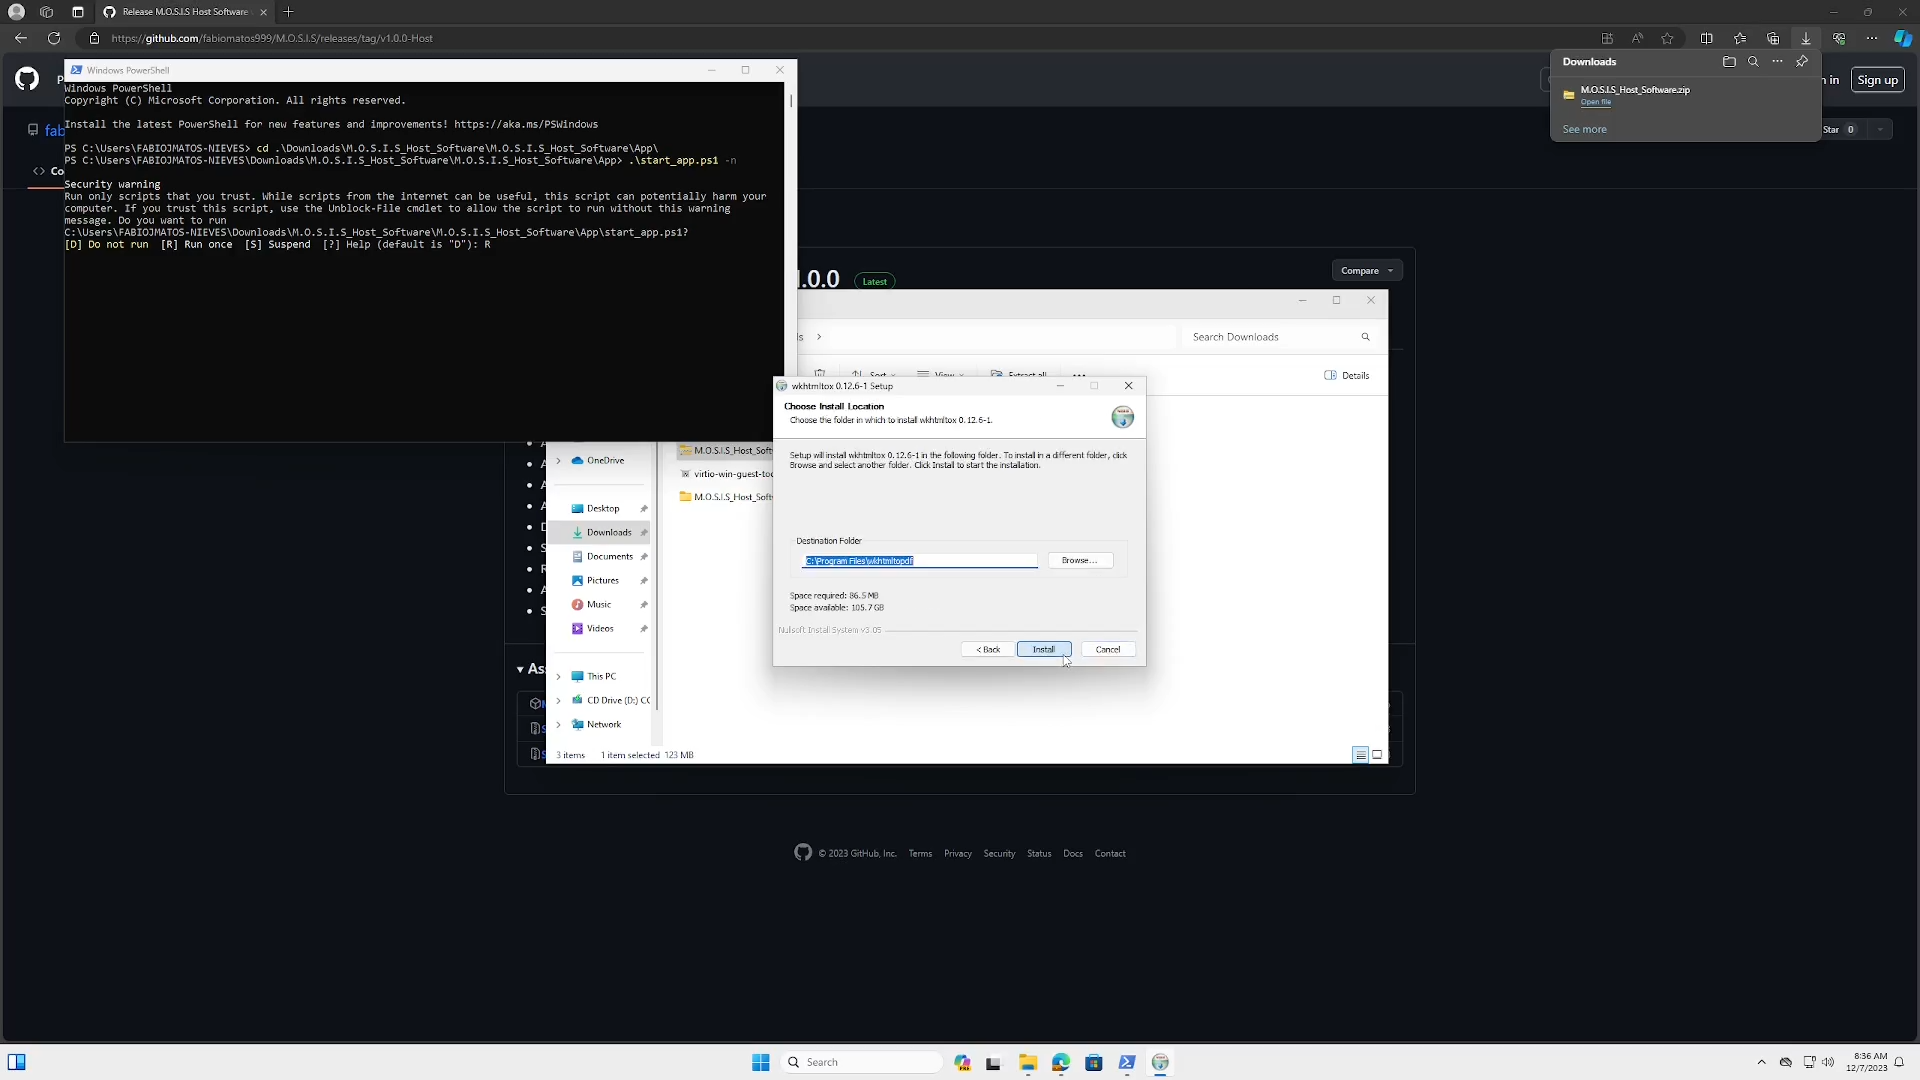
\includegraphics[width=\textwidth]{Figures/Windows-wkhtmltopdf-Menu-2.png}
		      \end{figure}
		\item Wait for the installer to finish
		      \begin{figure}[H]
			      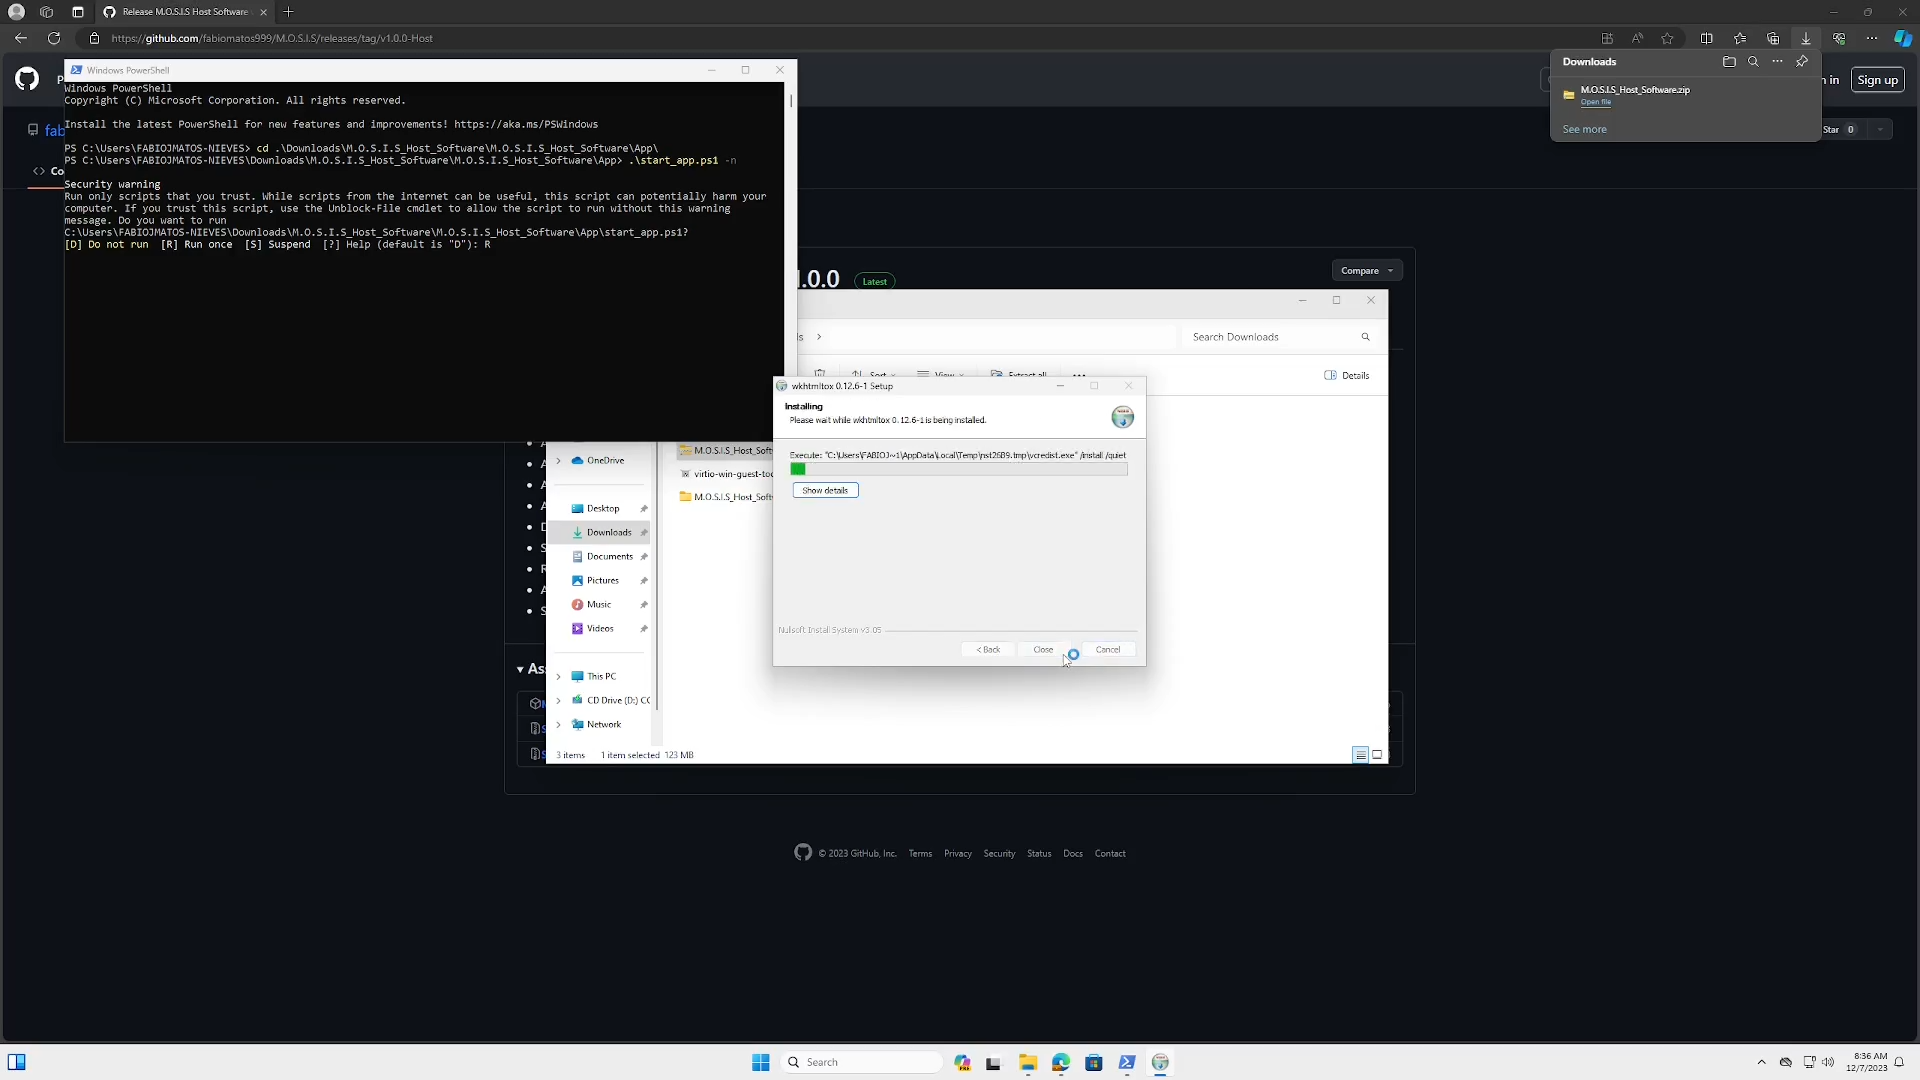
\includegraphics[width=\textwidth]{Figures/Windows-wkhtmltopdf-Menu-3.png}
		      \end{figure}
		\item Once the installer finishes, click on the close button
		      \begin{figure}[H]
			      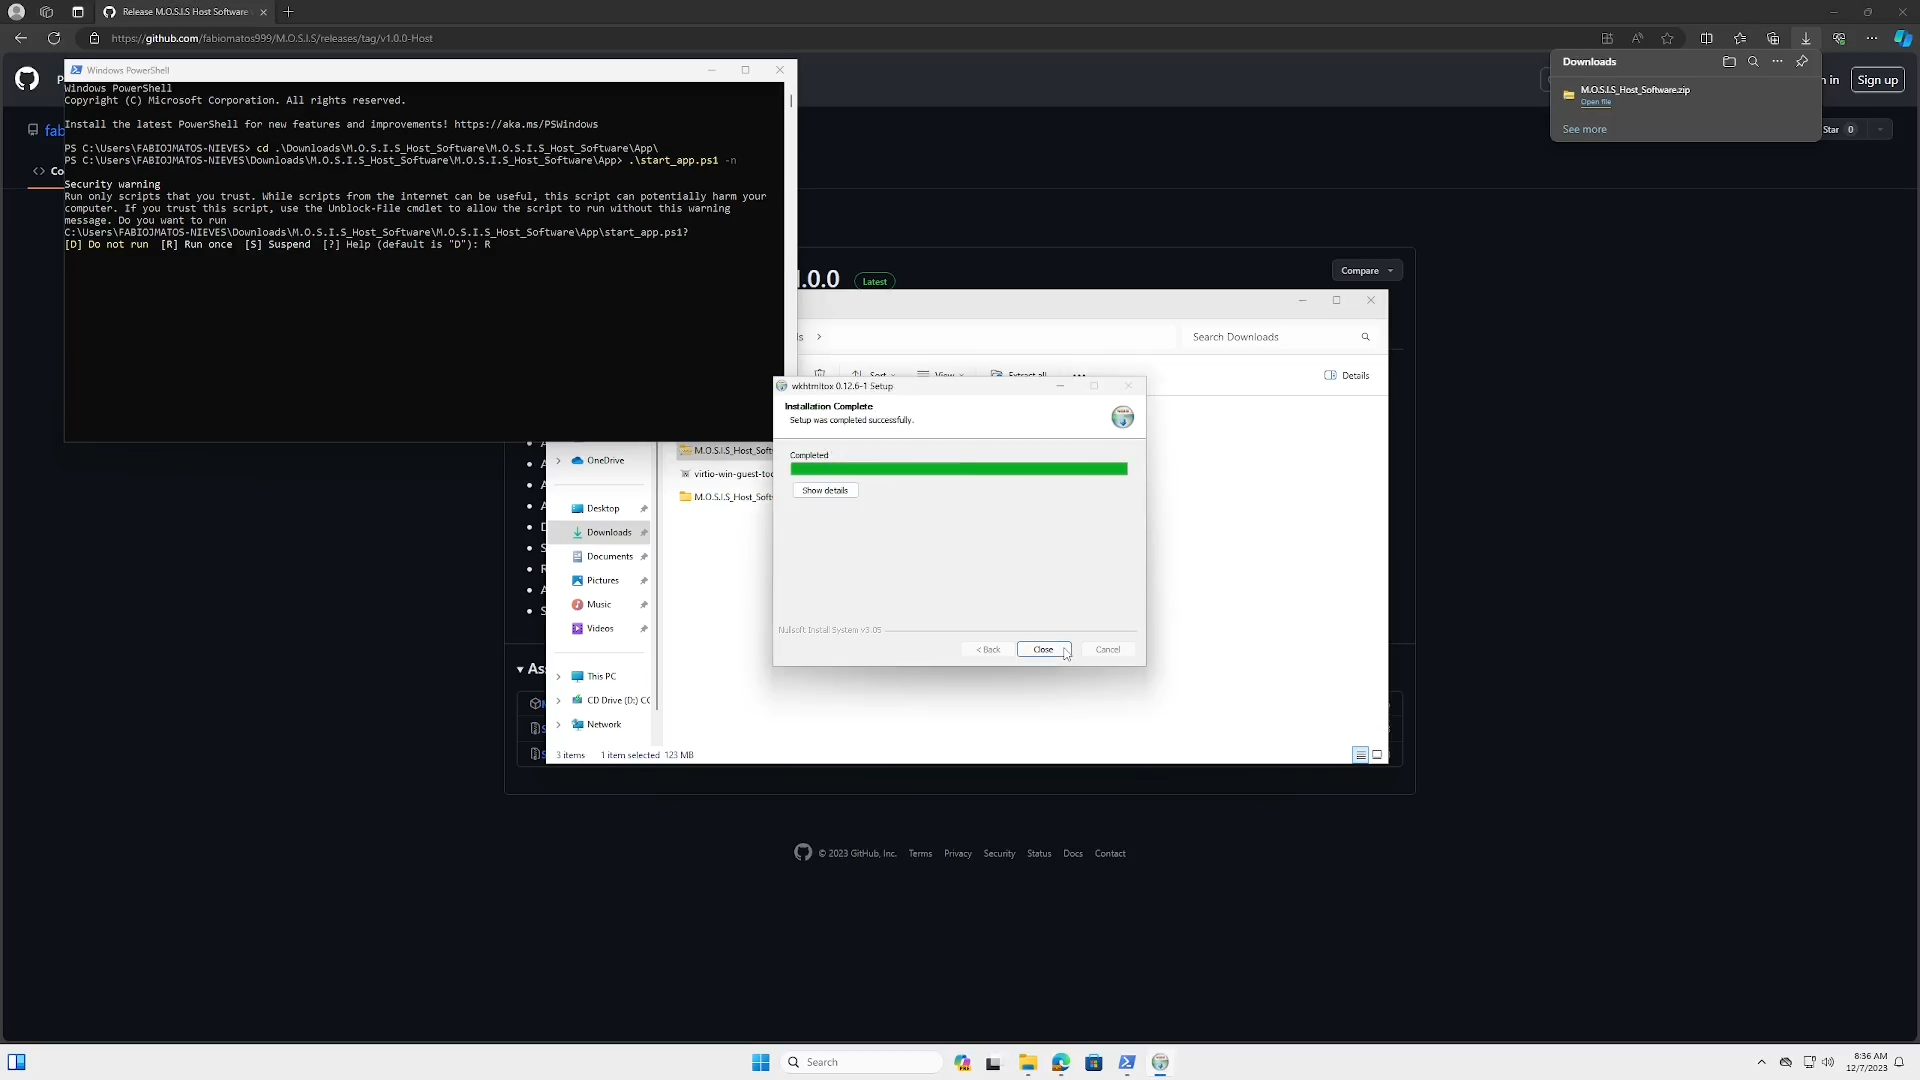
\includegraphics[width=\textwidth]{Figures/Windows-wkhtmltopdf-Menu-3-Close.png}
		      \end{figure}
		\item If prompted by the following screen, click ``yes''
		      \begin{figure}[H]
			      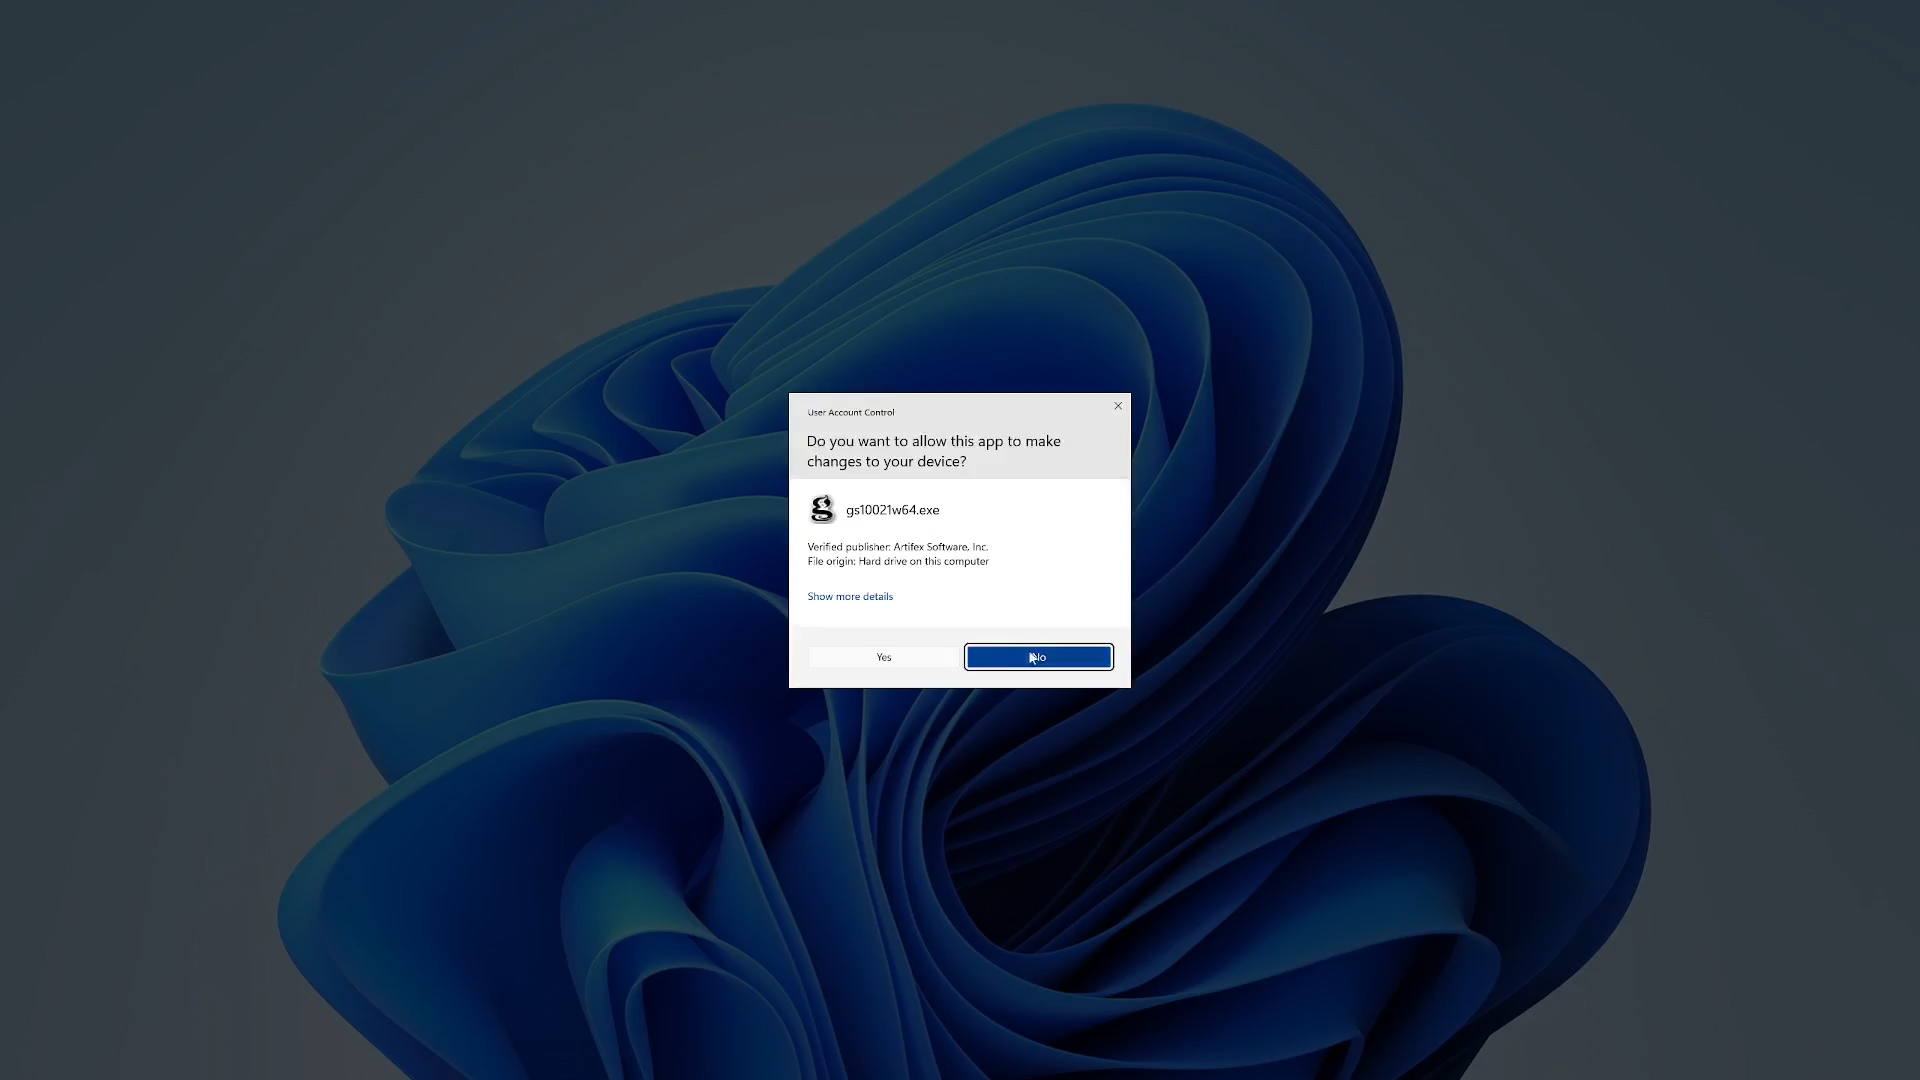
\includegraphics[width=\textwidth]{Figures/Windows-UAC-Ghostscript.png}
		      \end{figure}
		\item Once the following screen appears, click on the ``next'' button.
		      \begin{figure}[H]
			      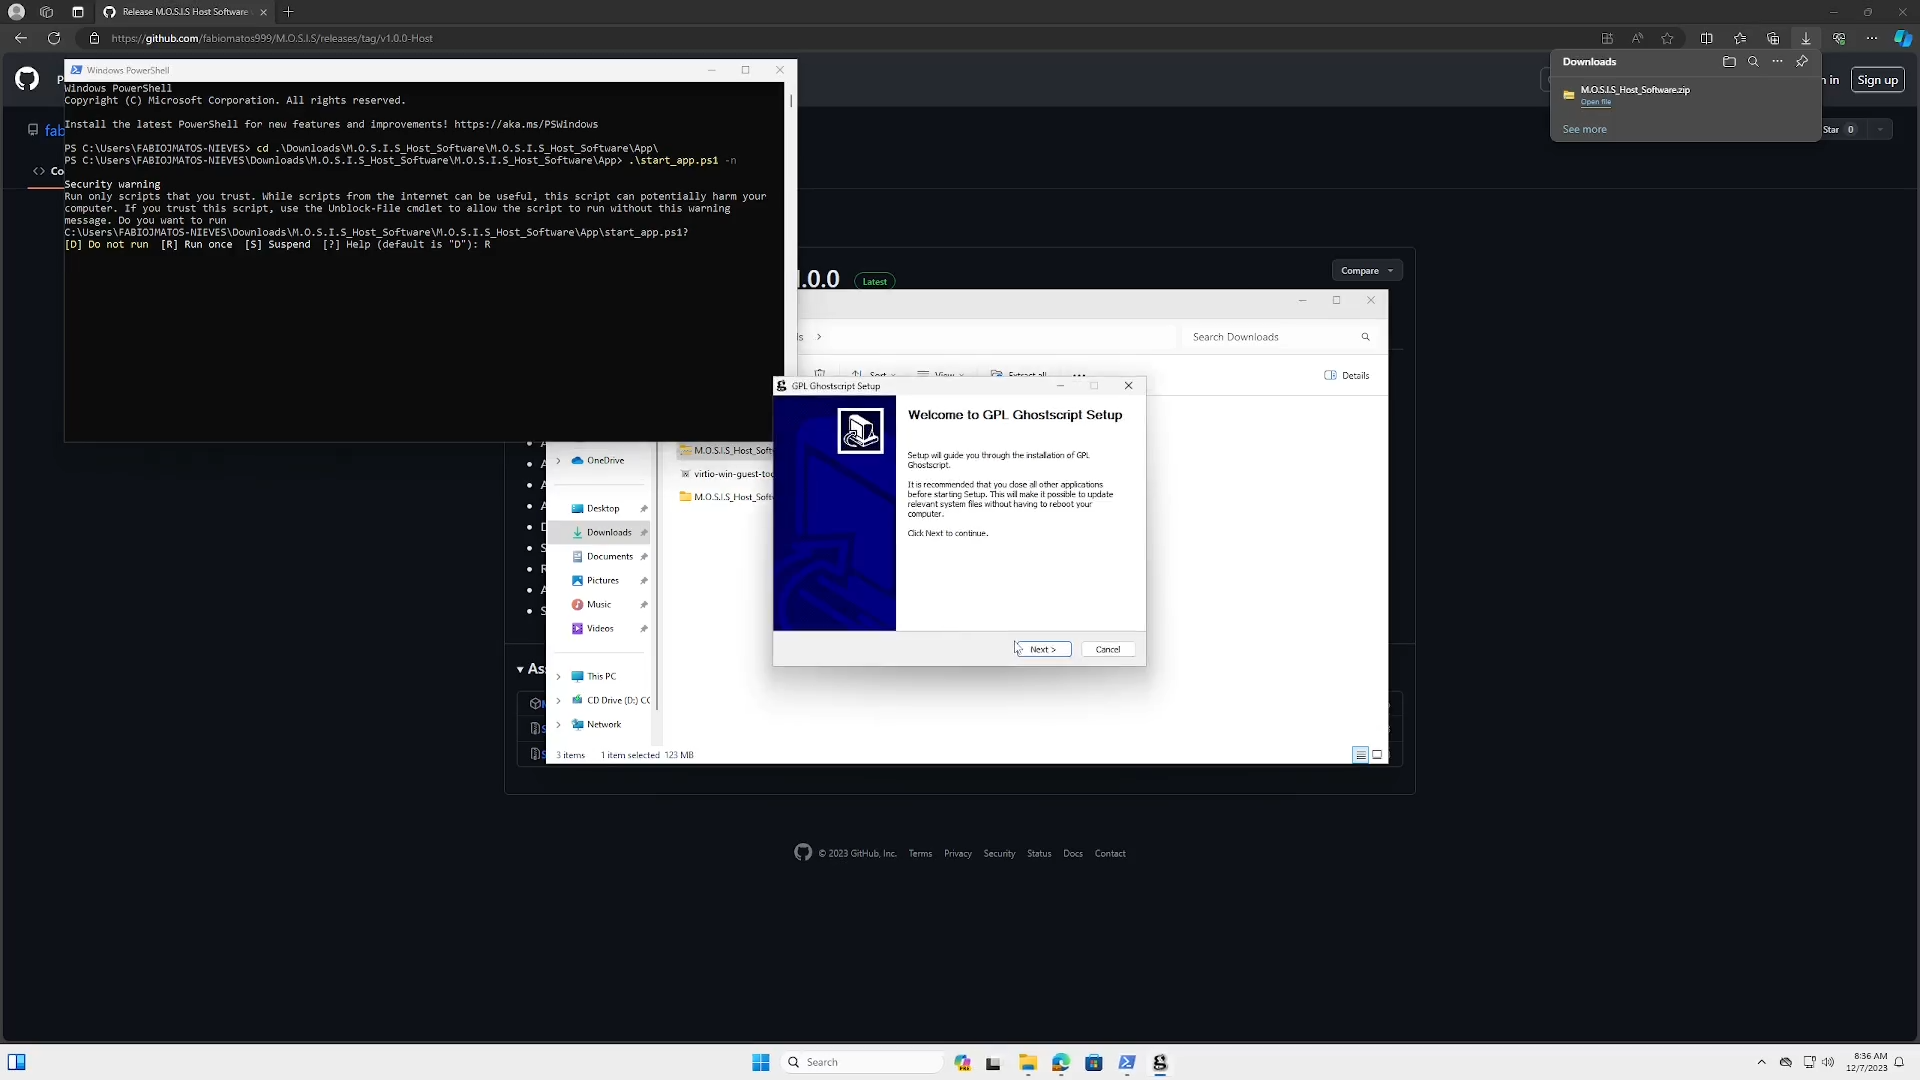
\includegraphics[width=\textwidth]{Figures/Windows-Ghostscript-Menu-1.png}
		      \end{figure}
		\item Click on the ``I agree'' button
		      \begin{figure}[H]
			      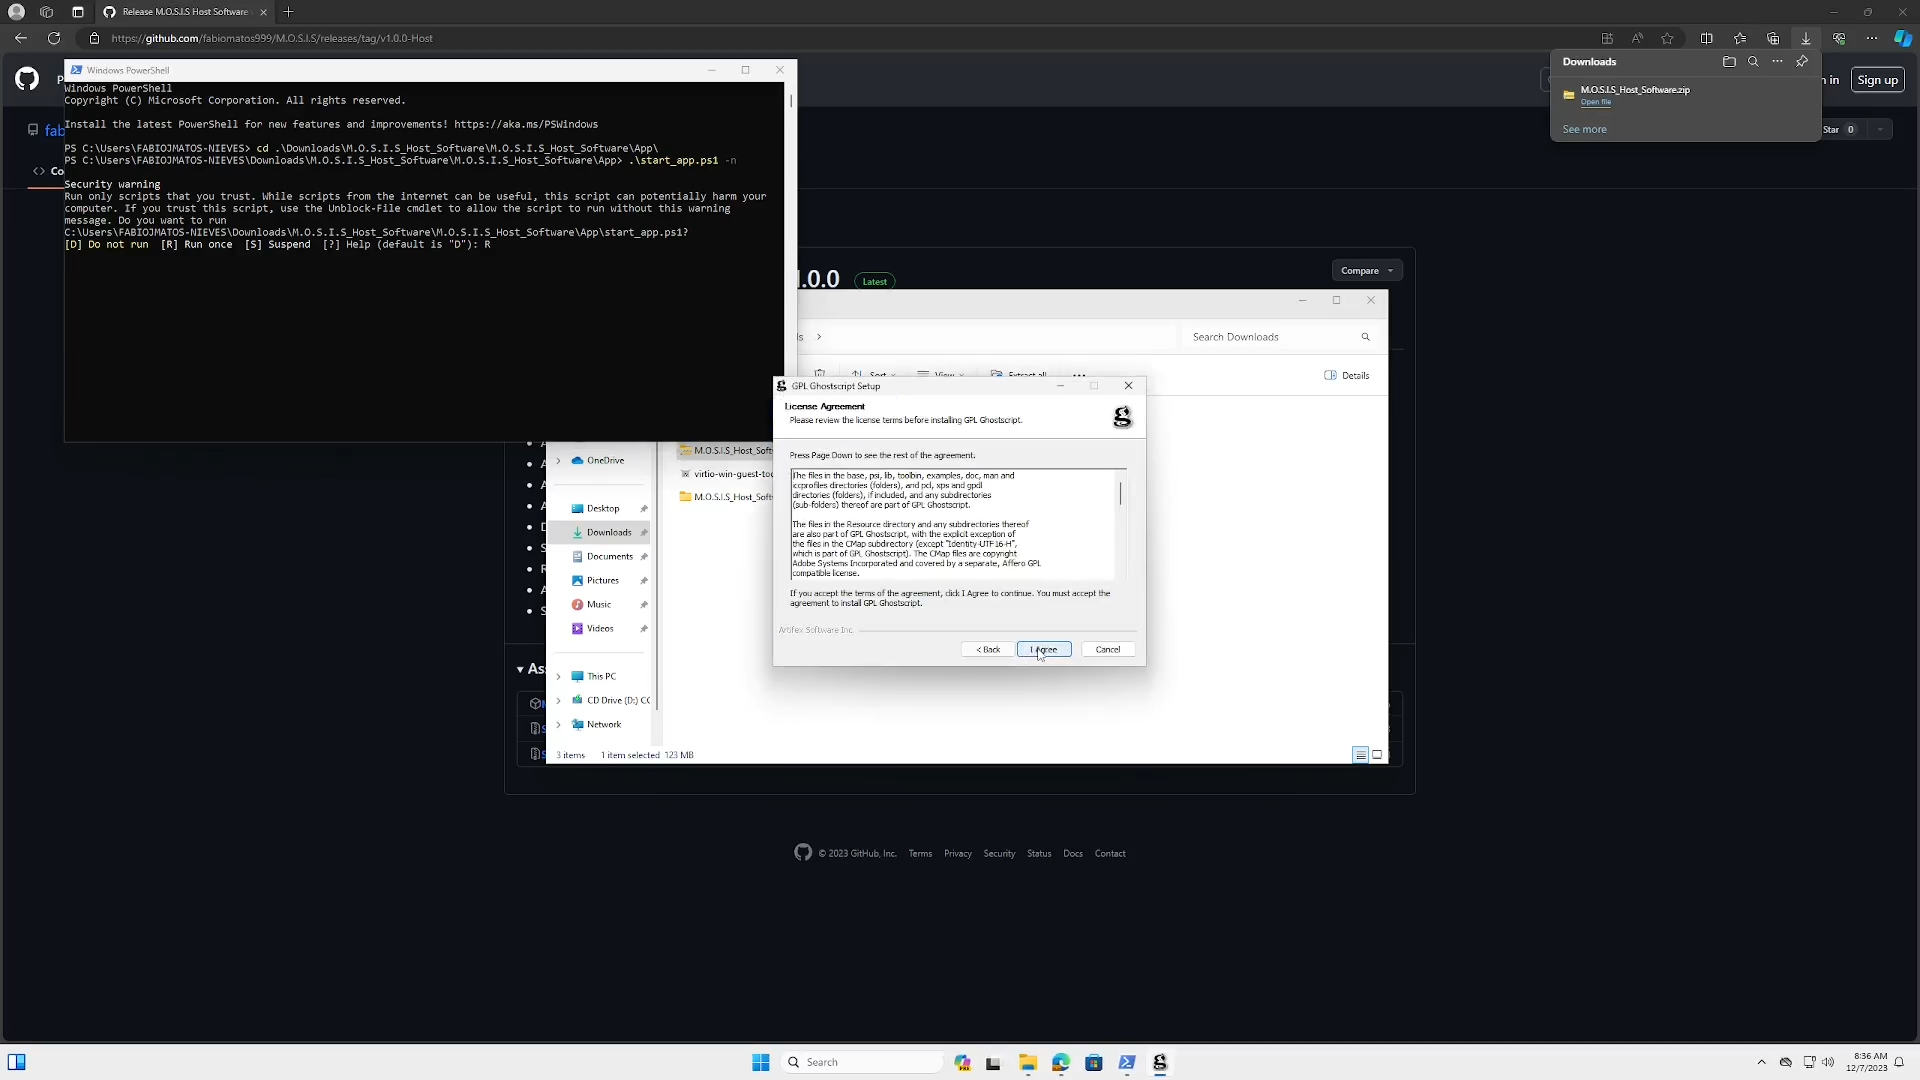
\includegraphics[width=\textwidth]{Figures/Windows-Ghostscript-Menu-2.png}
		      \end{figure}
		\item Wait for the installer to complete
		      \begin{figure}[H]
			      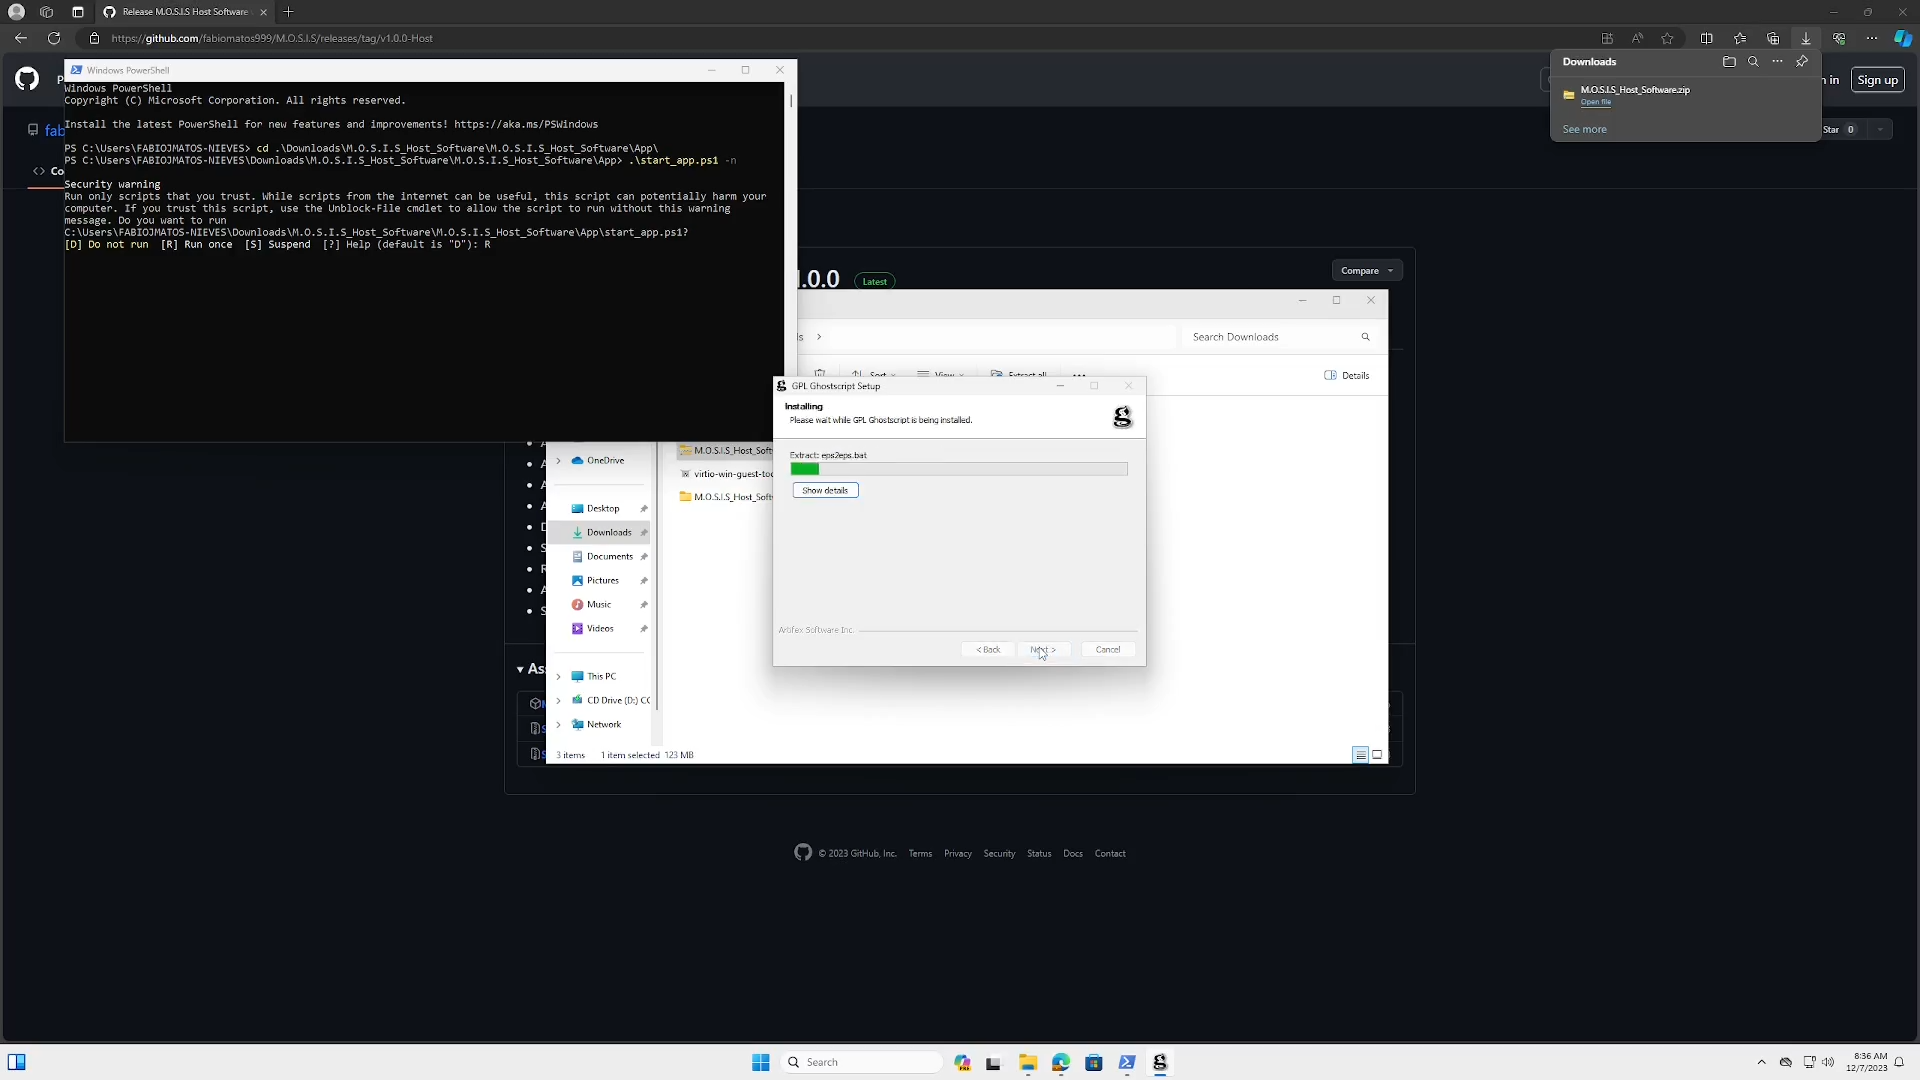
\includegraphics[width=\textwidth]{Figures/Windows-Ghostscript-Menu-3.png}
		      \end{figure}
		\item Click on the ``Finish'' button.
		      \begin{figure}[H]
			      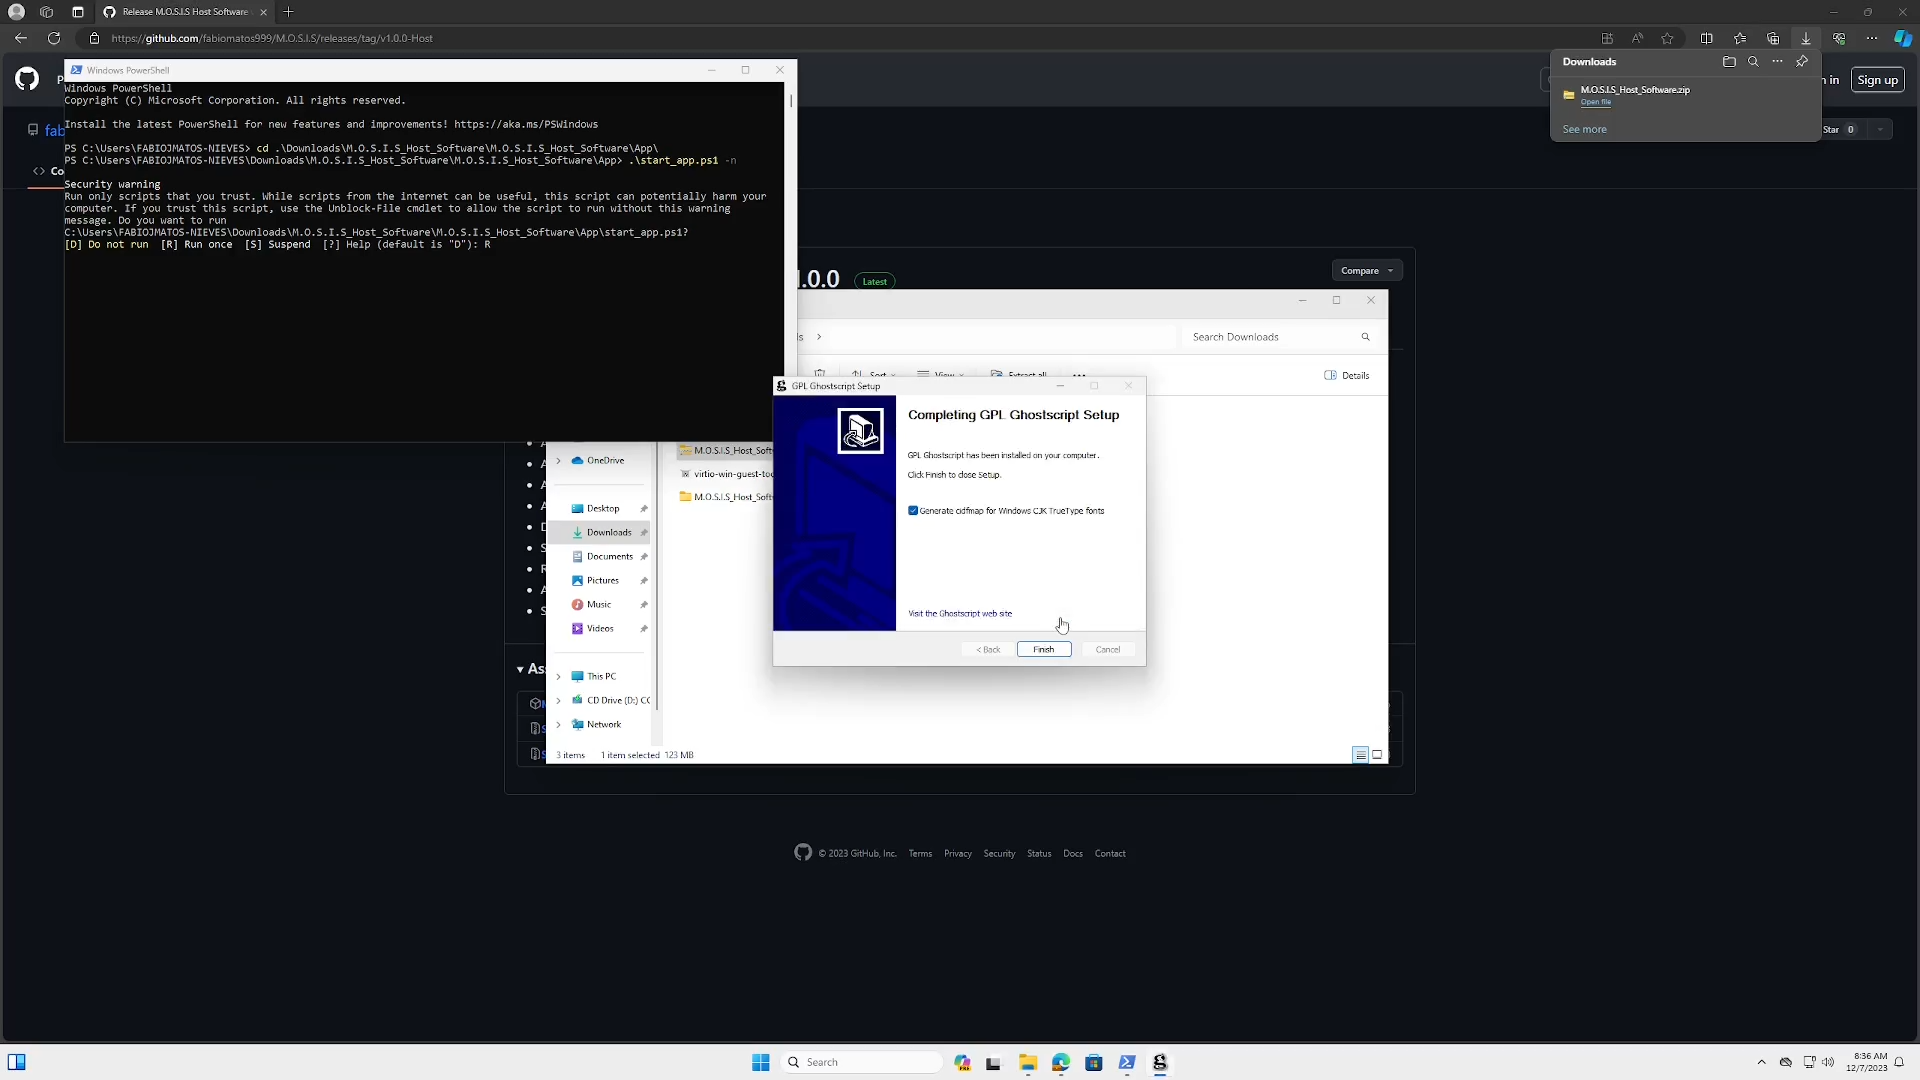
\includegraphics[width=\textwidth]{Figures/Windows-Ghostscript-Menu-4.png}
		      \end{figure}
		\item Once the following screen appears, click on the ``OK'' button.
		      \begin{figure}[H]
			      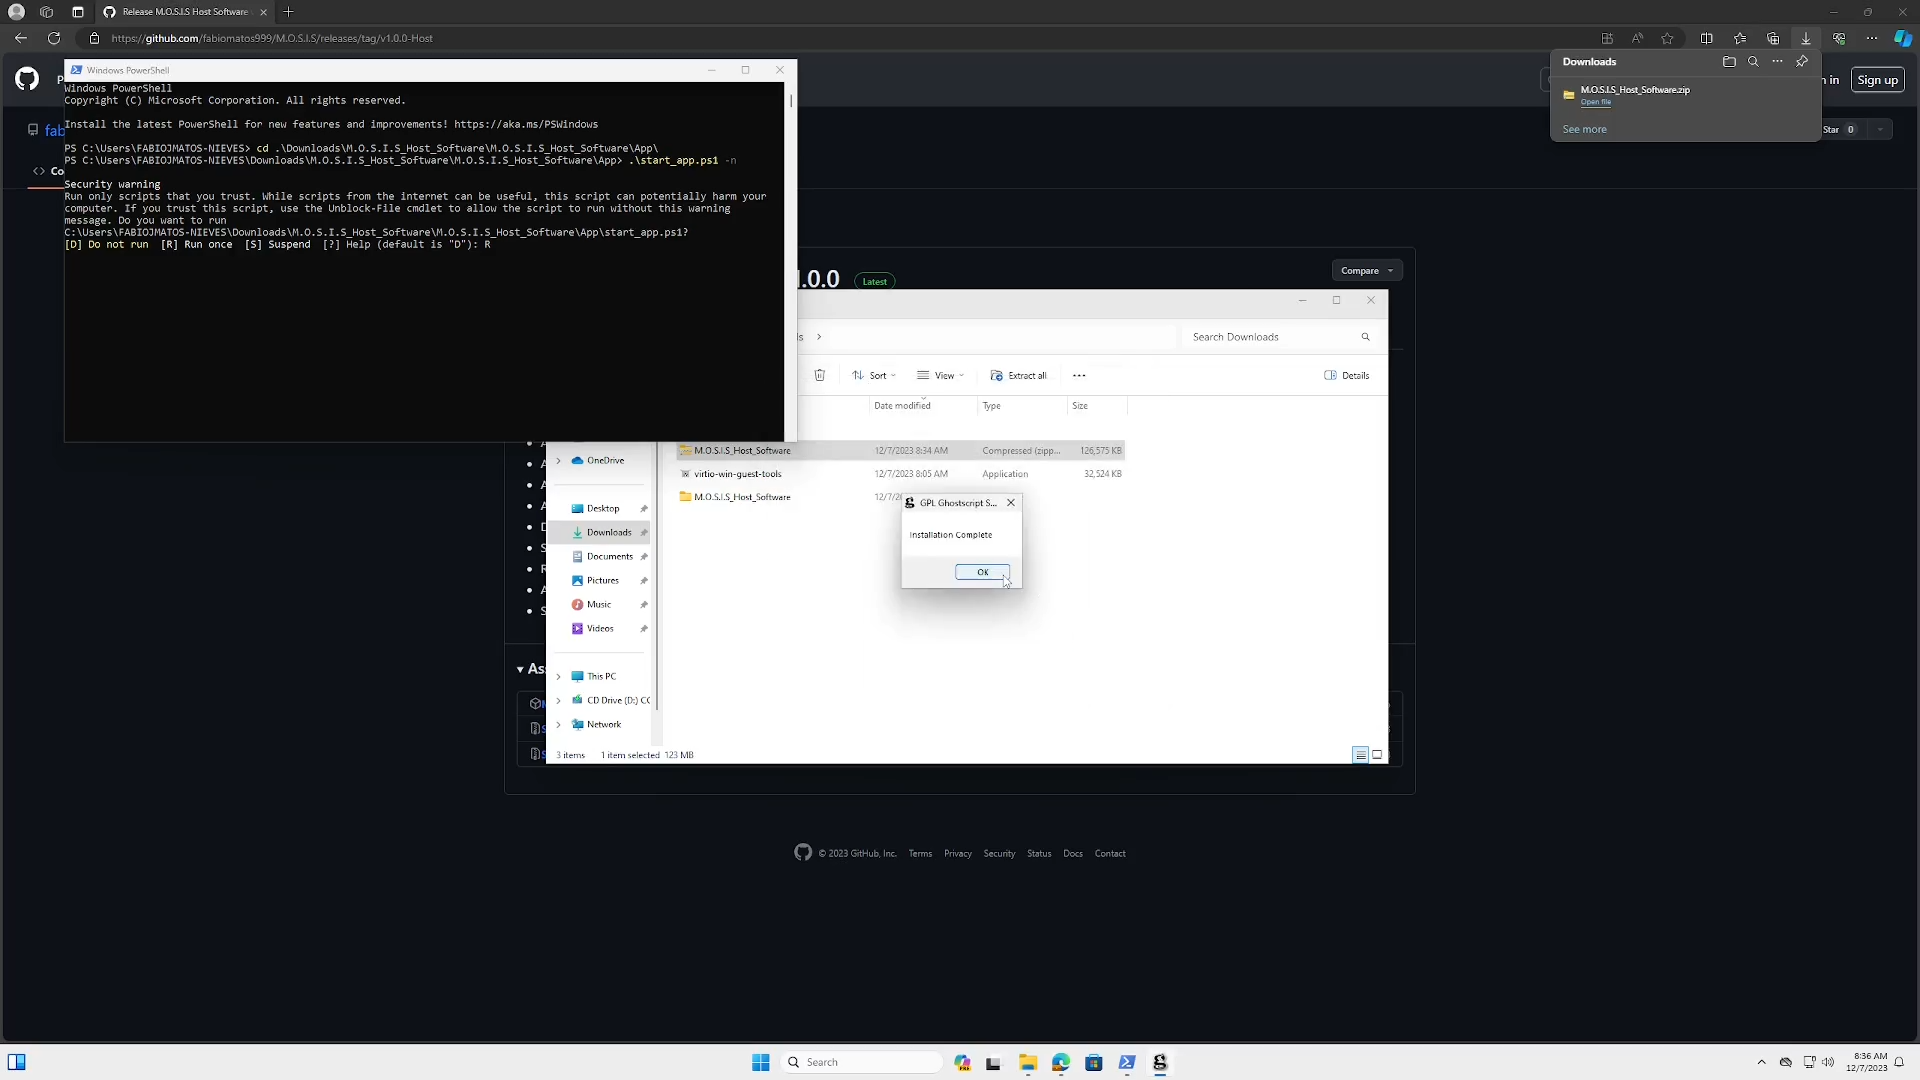
\includegraphics[width=\textwidth]{Figures/Windows-Ghostscript-Menu-5.png}
		      \end{figure}
		\item Once the following installer appears, make sure the ``Use admin privileges when installing py.exe'' and ``Add python.exe to PATH'' and click on the ``Install Now'' button.
		      \begin{figure}[H]
			      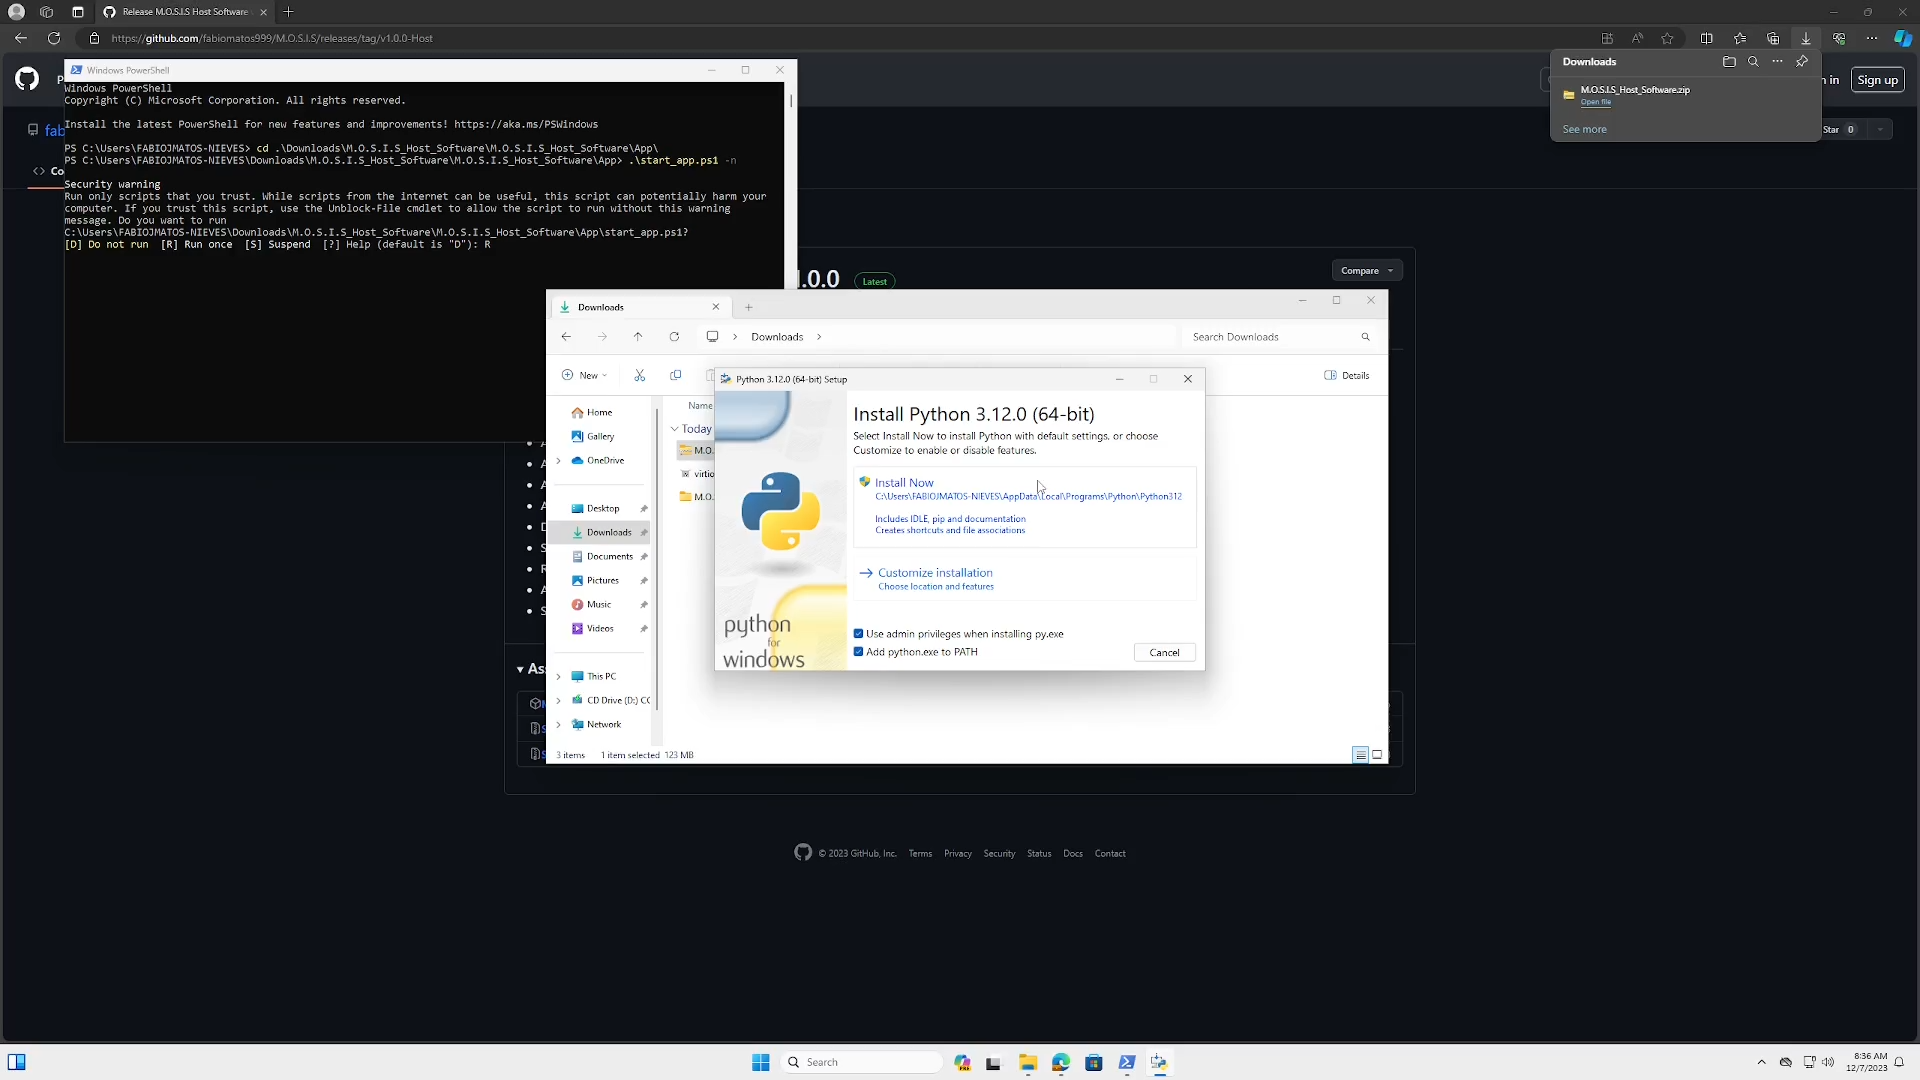
\includegraphics[width=\textwidth]{Figures/Windows-Python-Menu-1.png}
		      \end{figure}
		\item If prompted by the following screen, click ``yes''
		      \begin{figure}[H]
			      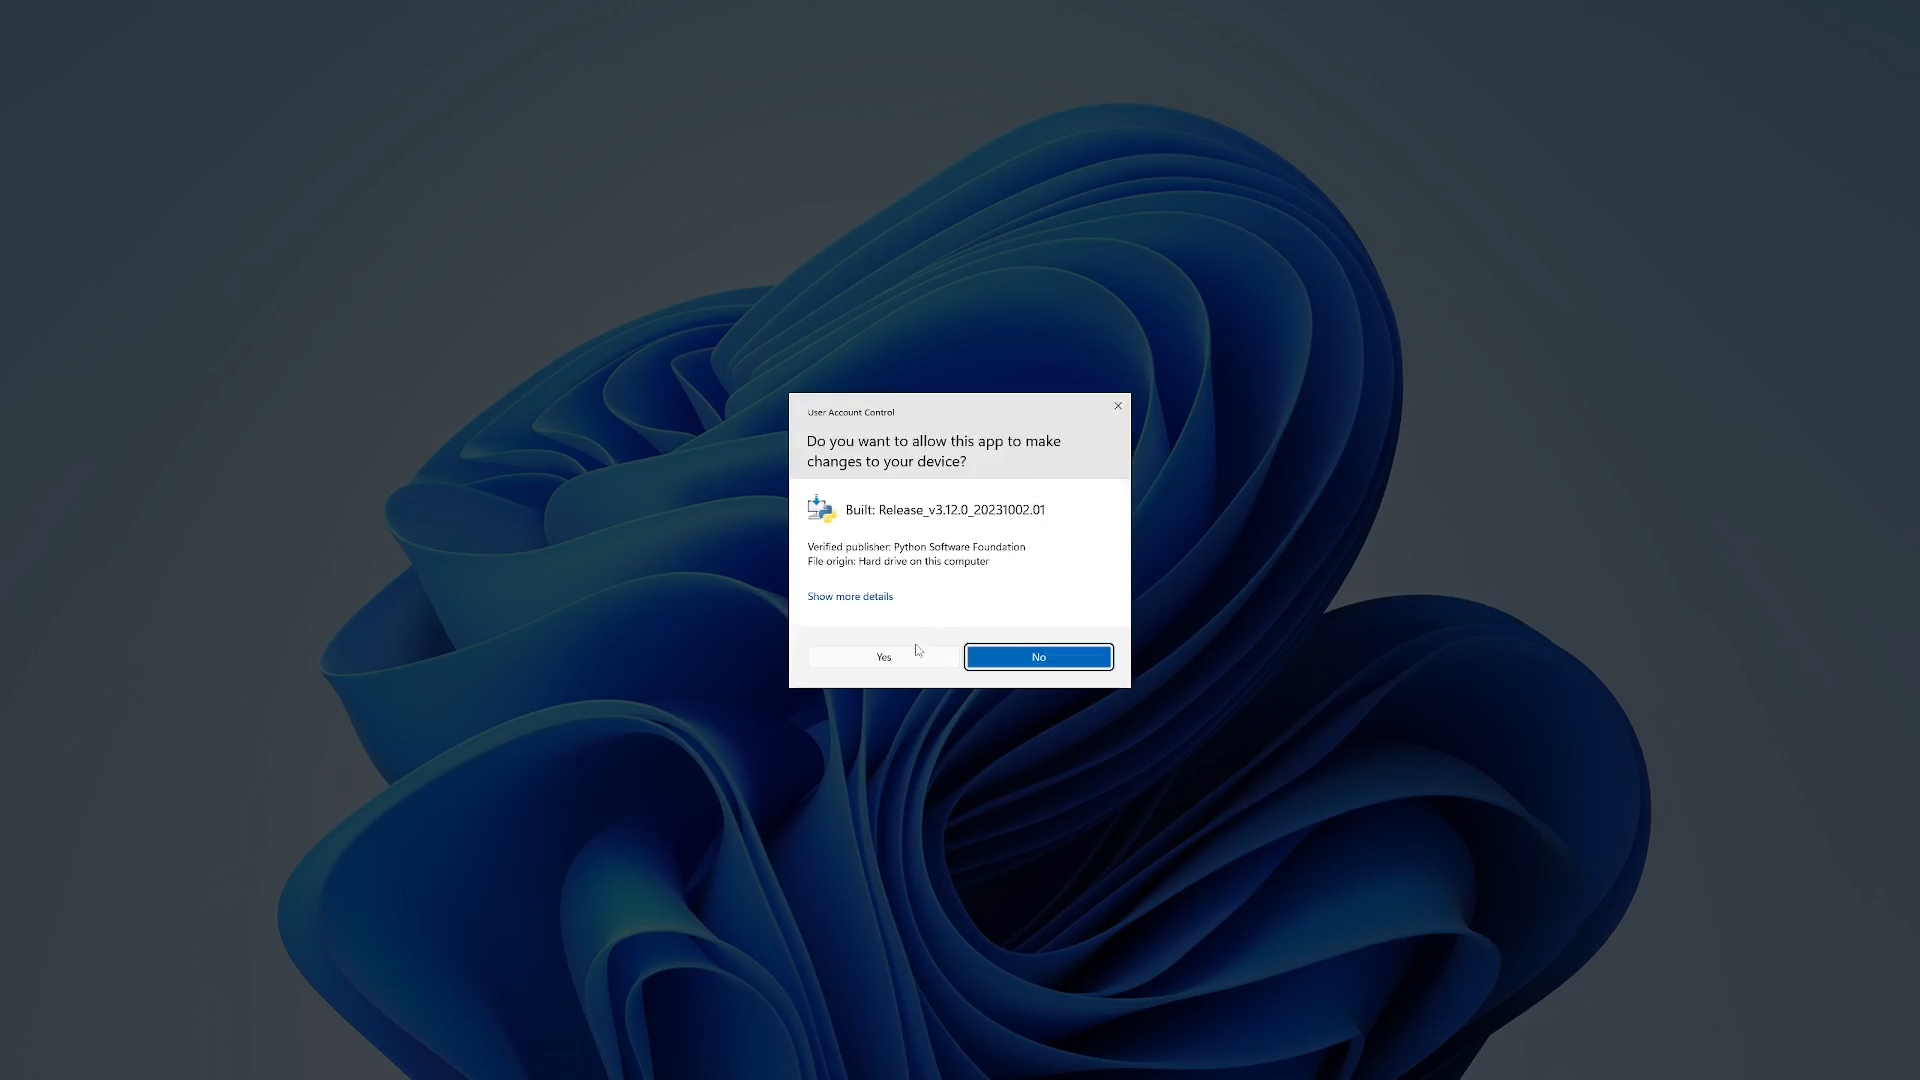
\includegraphics[width=\textwidth]{Figures/Windows-UAC-Python-1.png}
		      \end{figure}
		\item Wait for the installer to complete
		      \begin{figure}[H]
			      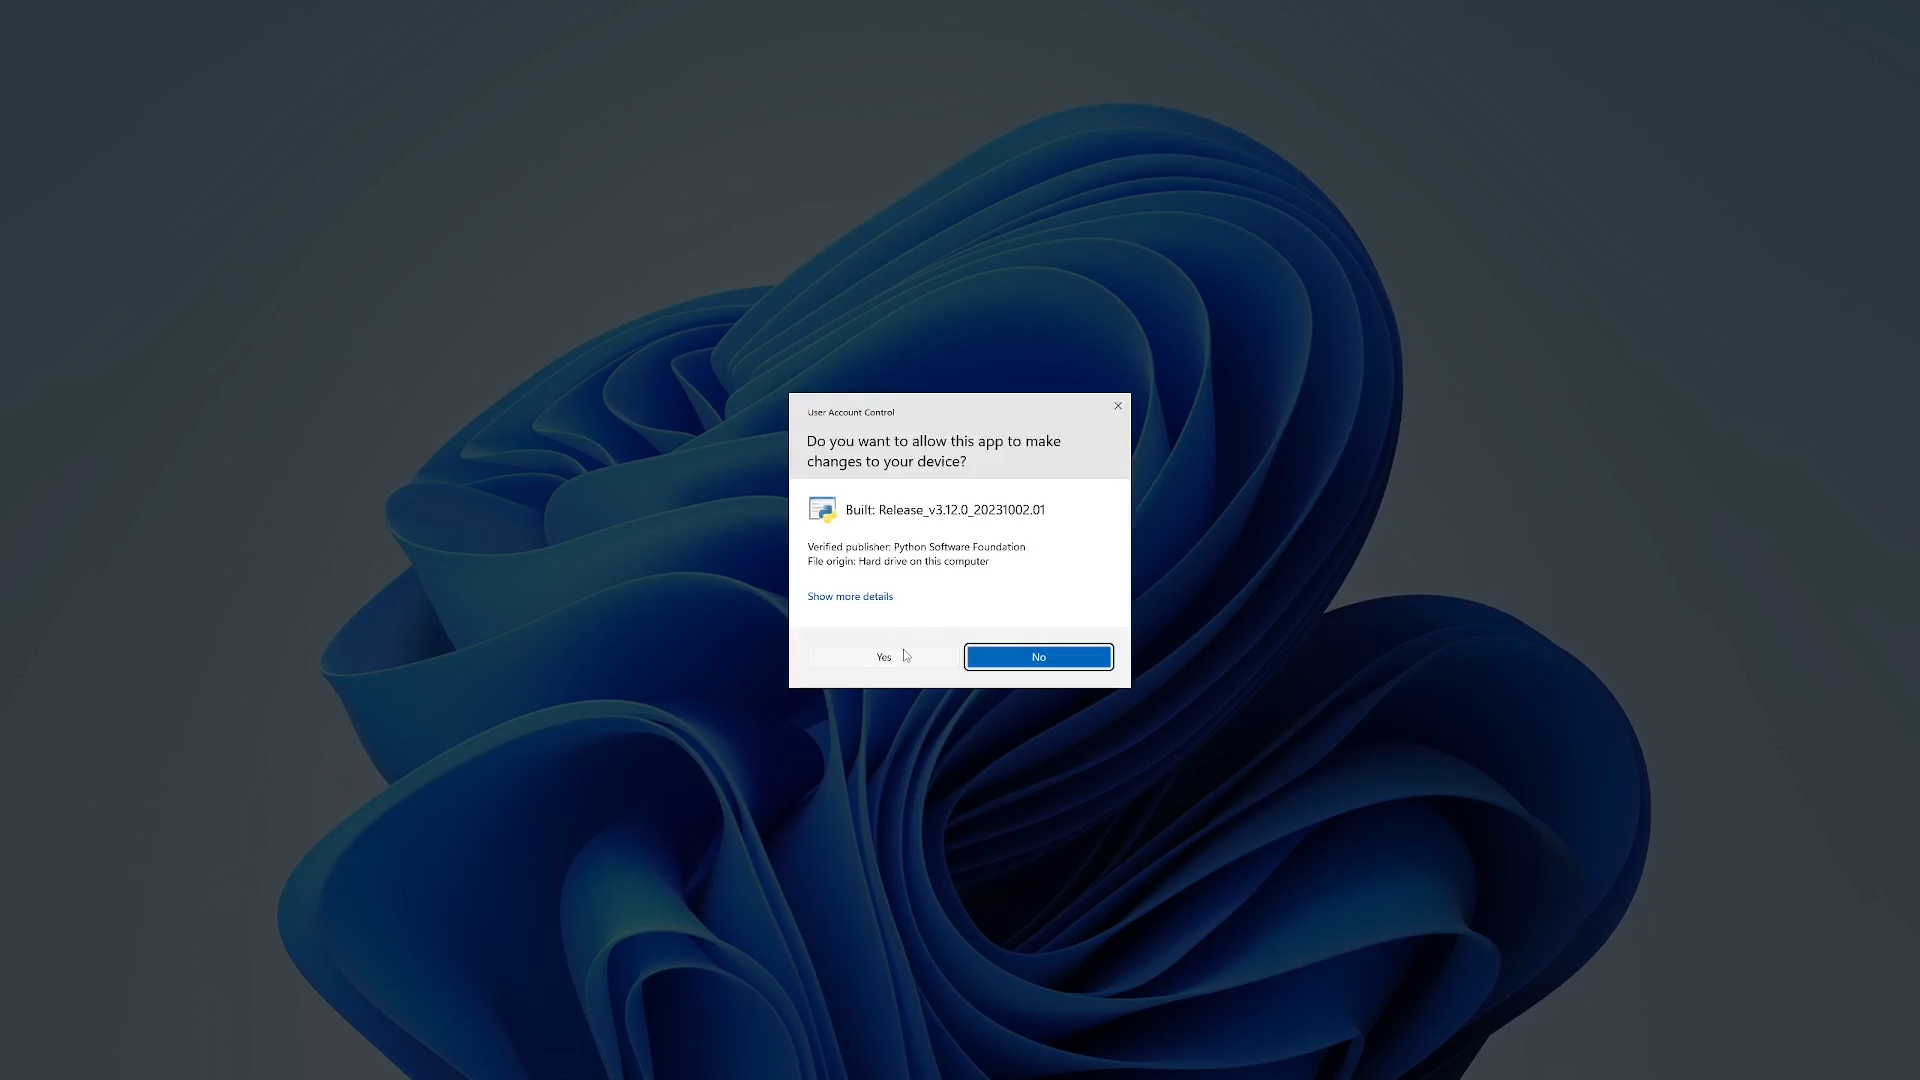
\includegraphics[width=\textwidth]{Figures/Windows-UAC-Python-2.png}
		      \end{figure}
		\item Once this menu appears, click on the ``Disable path length limit''
		      \begin{figure}[H]
			      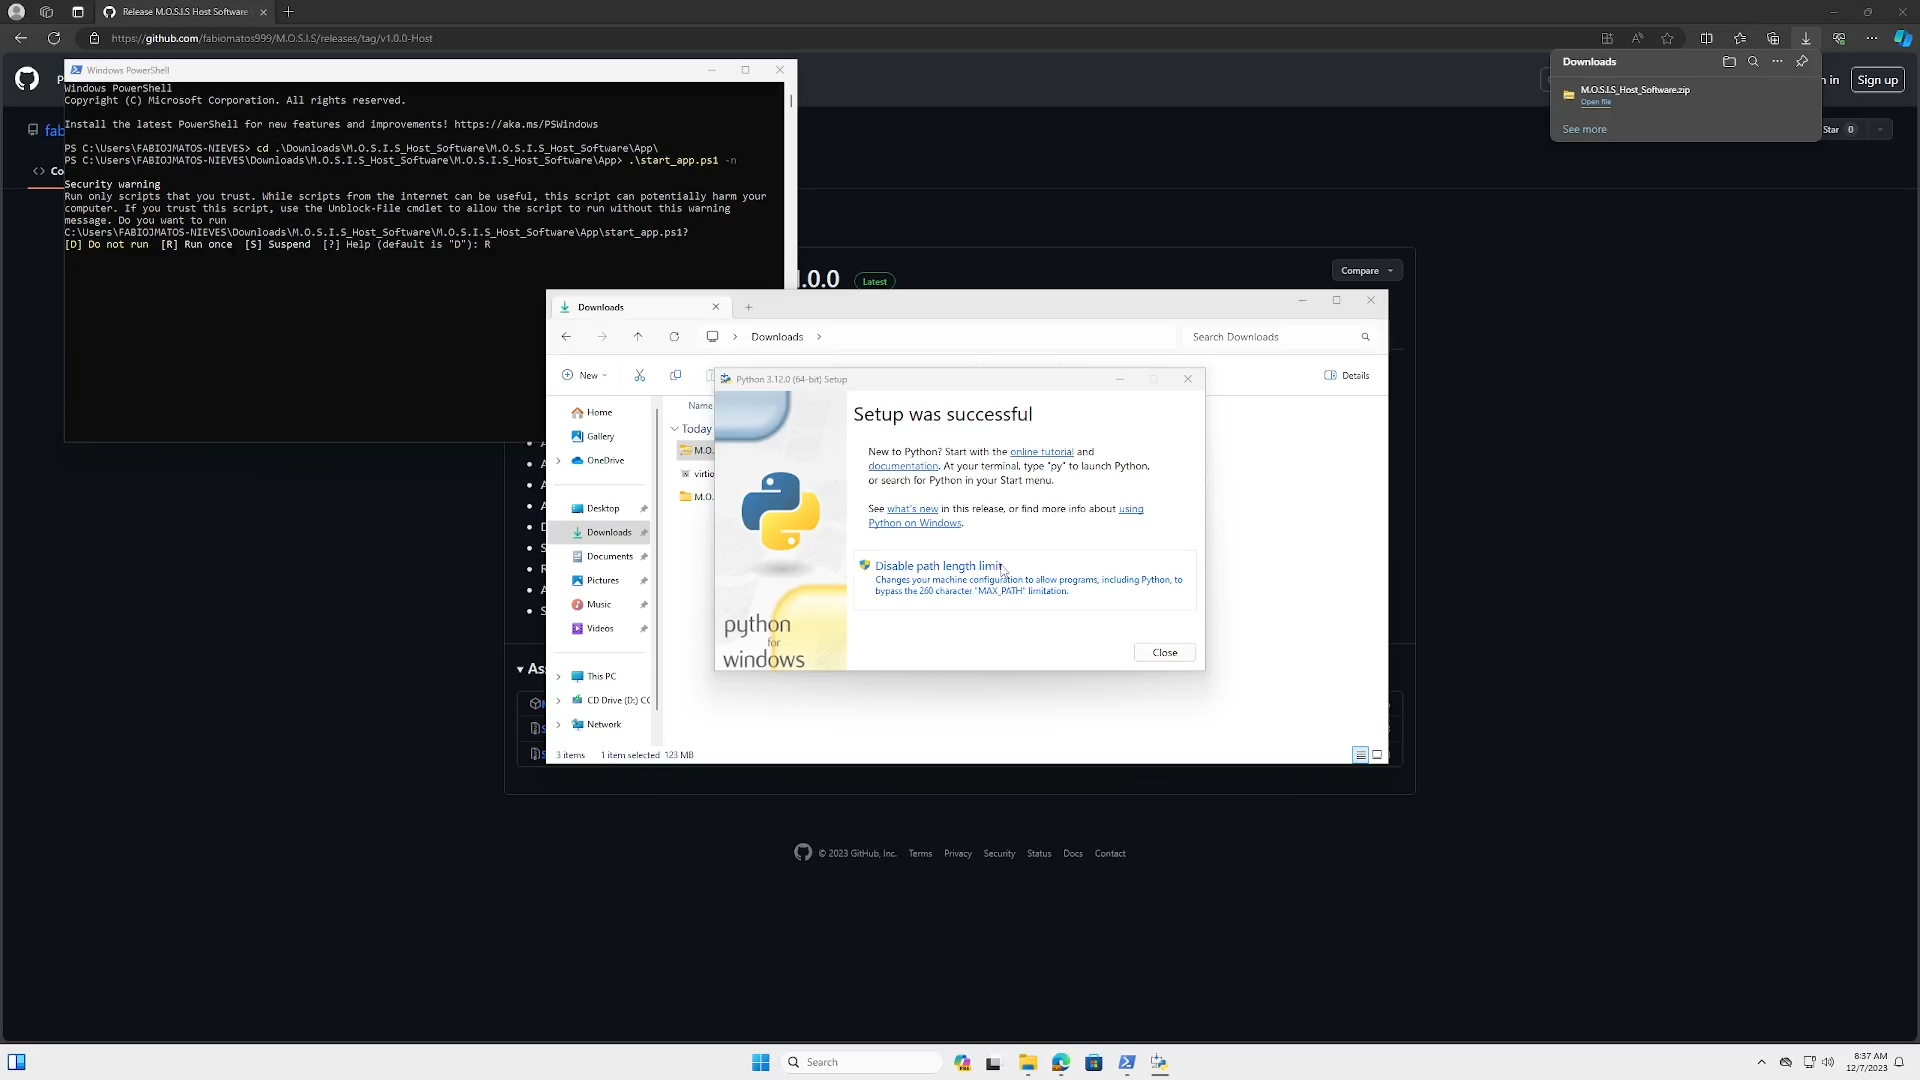
\includegraphics[width=\textwidth]{Figures/Windows-Python-Menu-3.png}
		      \end{figure}
		\item If prompted by the following screen, click ``yes''
		      \begin{figure}[H]
			      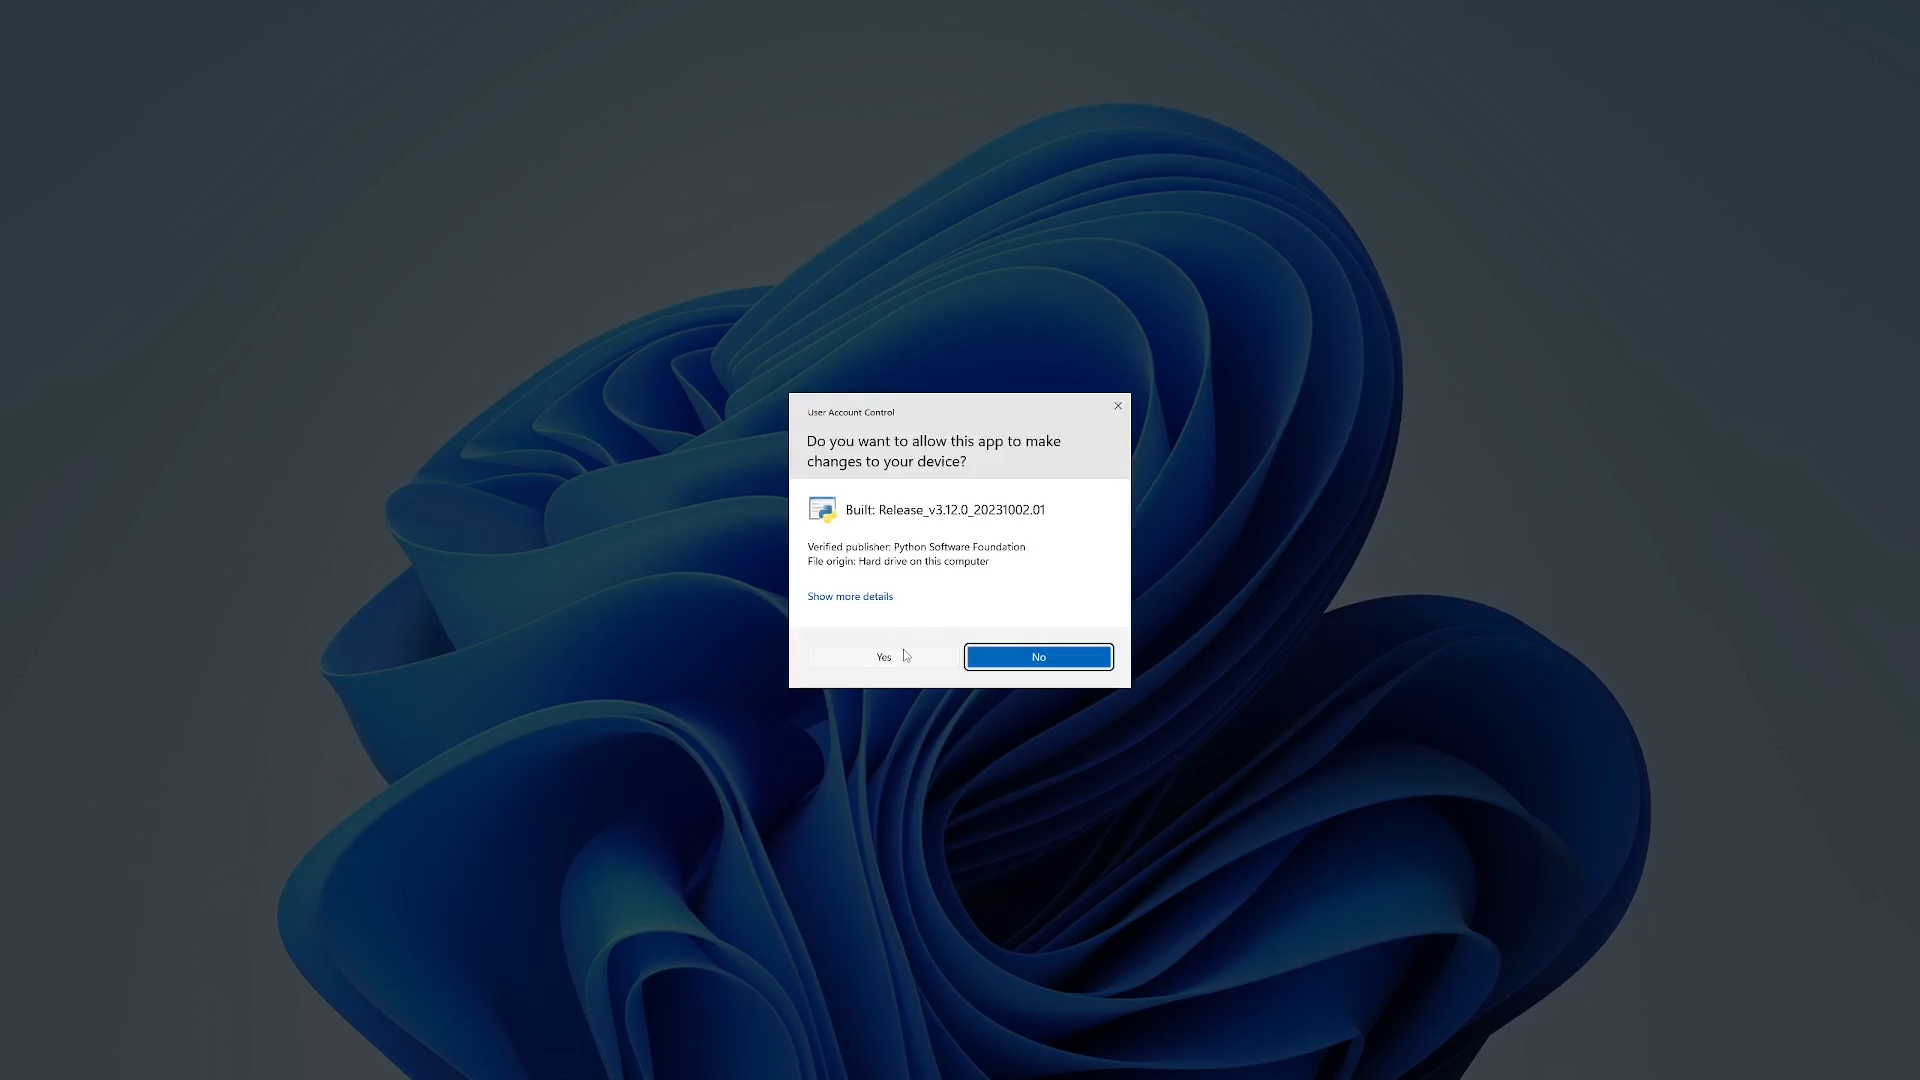
\includegraphics[width=\textwidth]{Figures/Windows-UAC-Python-2.png}
		      \end{figure}
		\item Once the Python installer completes, the Powershell should appear frozen for a couple of seconds and then print out a bunch of output
		      \begin{figure}[H]
			      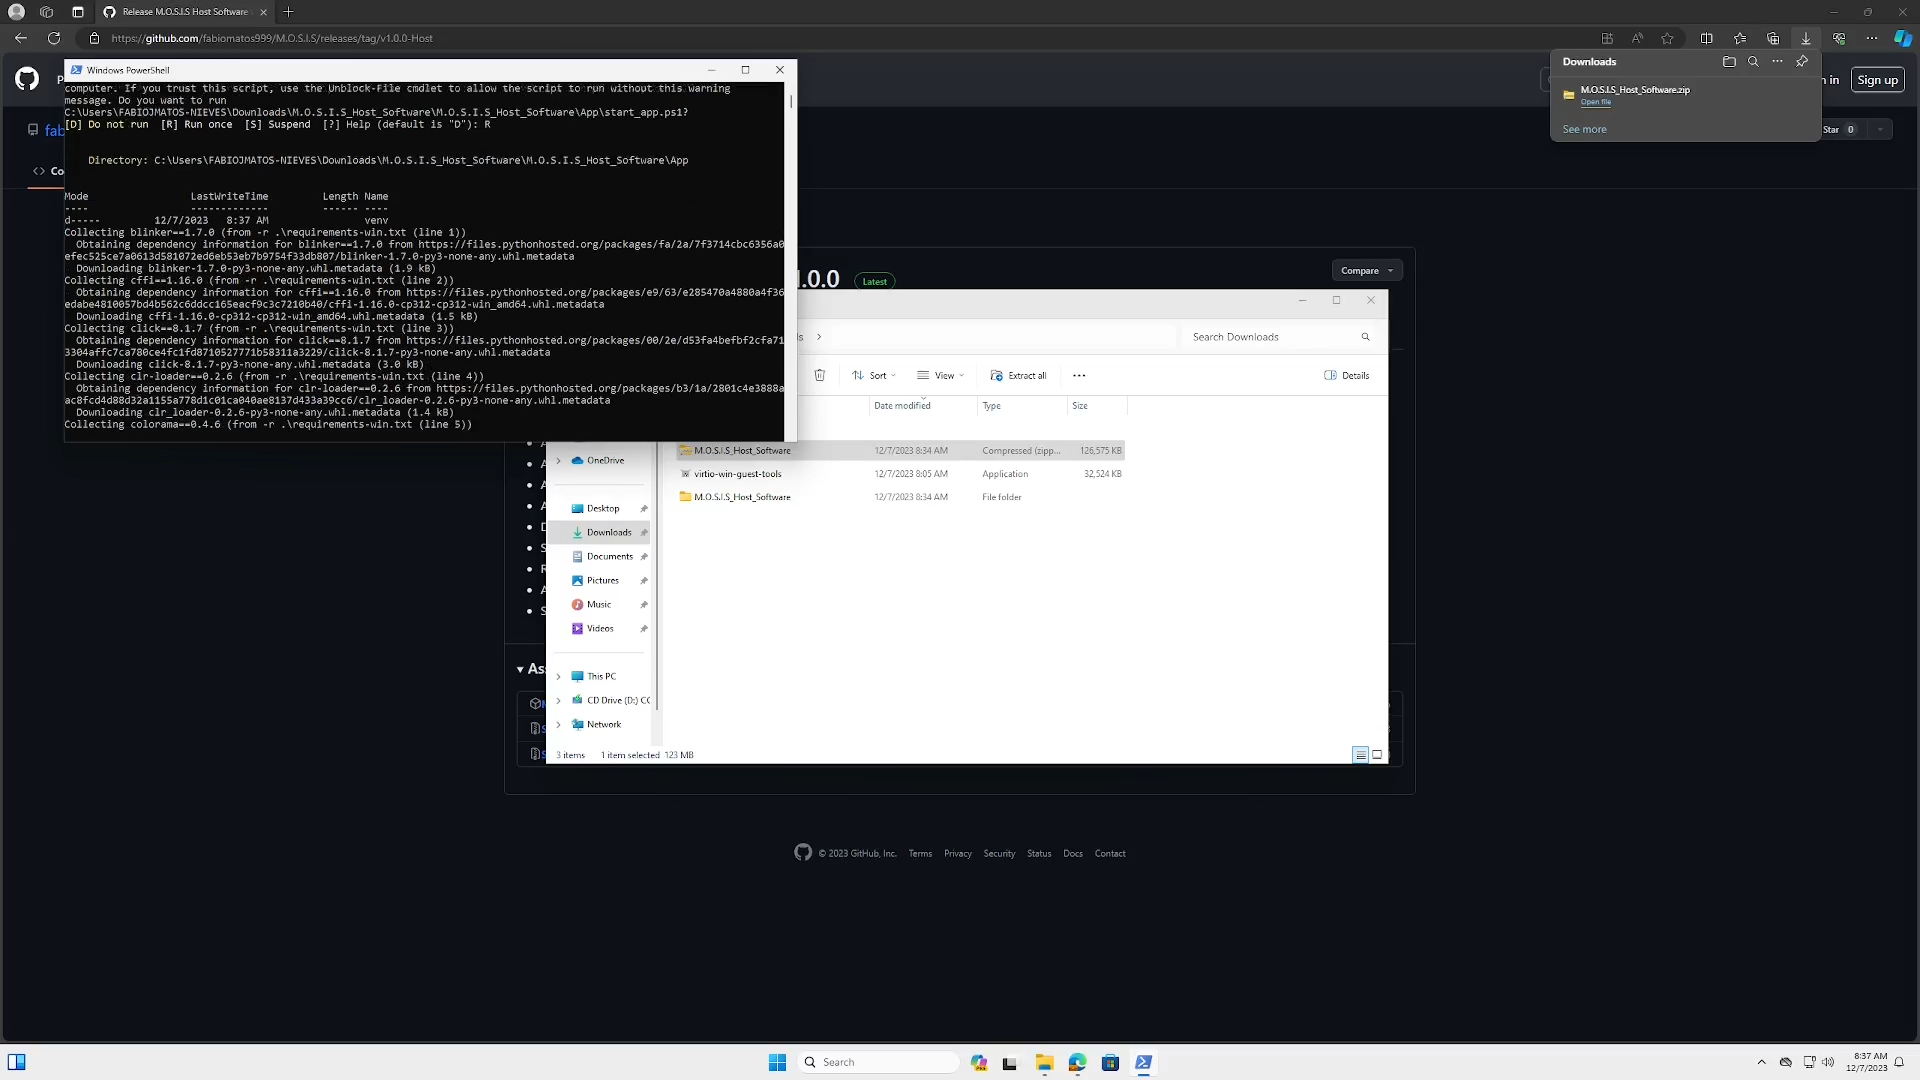
\includegraphics[width=\textwidth]{Figures/Windows-Poweshell-venv-install-1.png}
		      \end{figure}
		\item Once the host software finishes installing, the following screen may appear, if so click on the ``yes'' button
		      \begin{figure}[H]
			      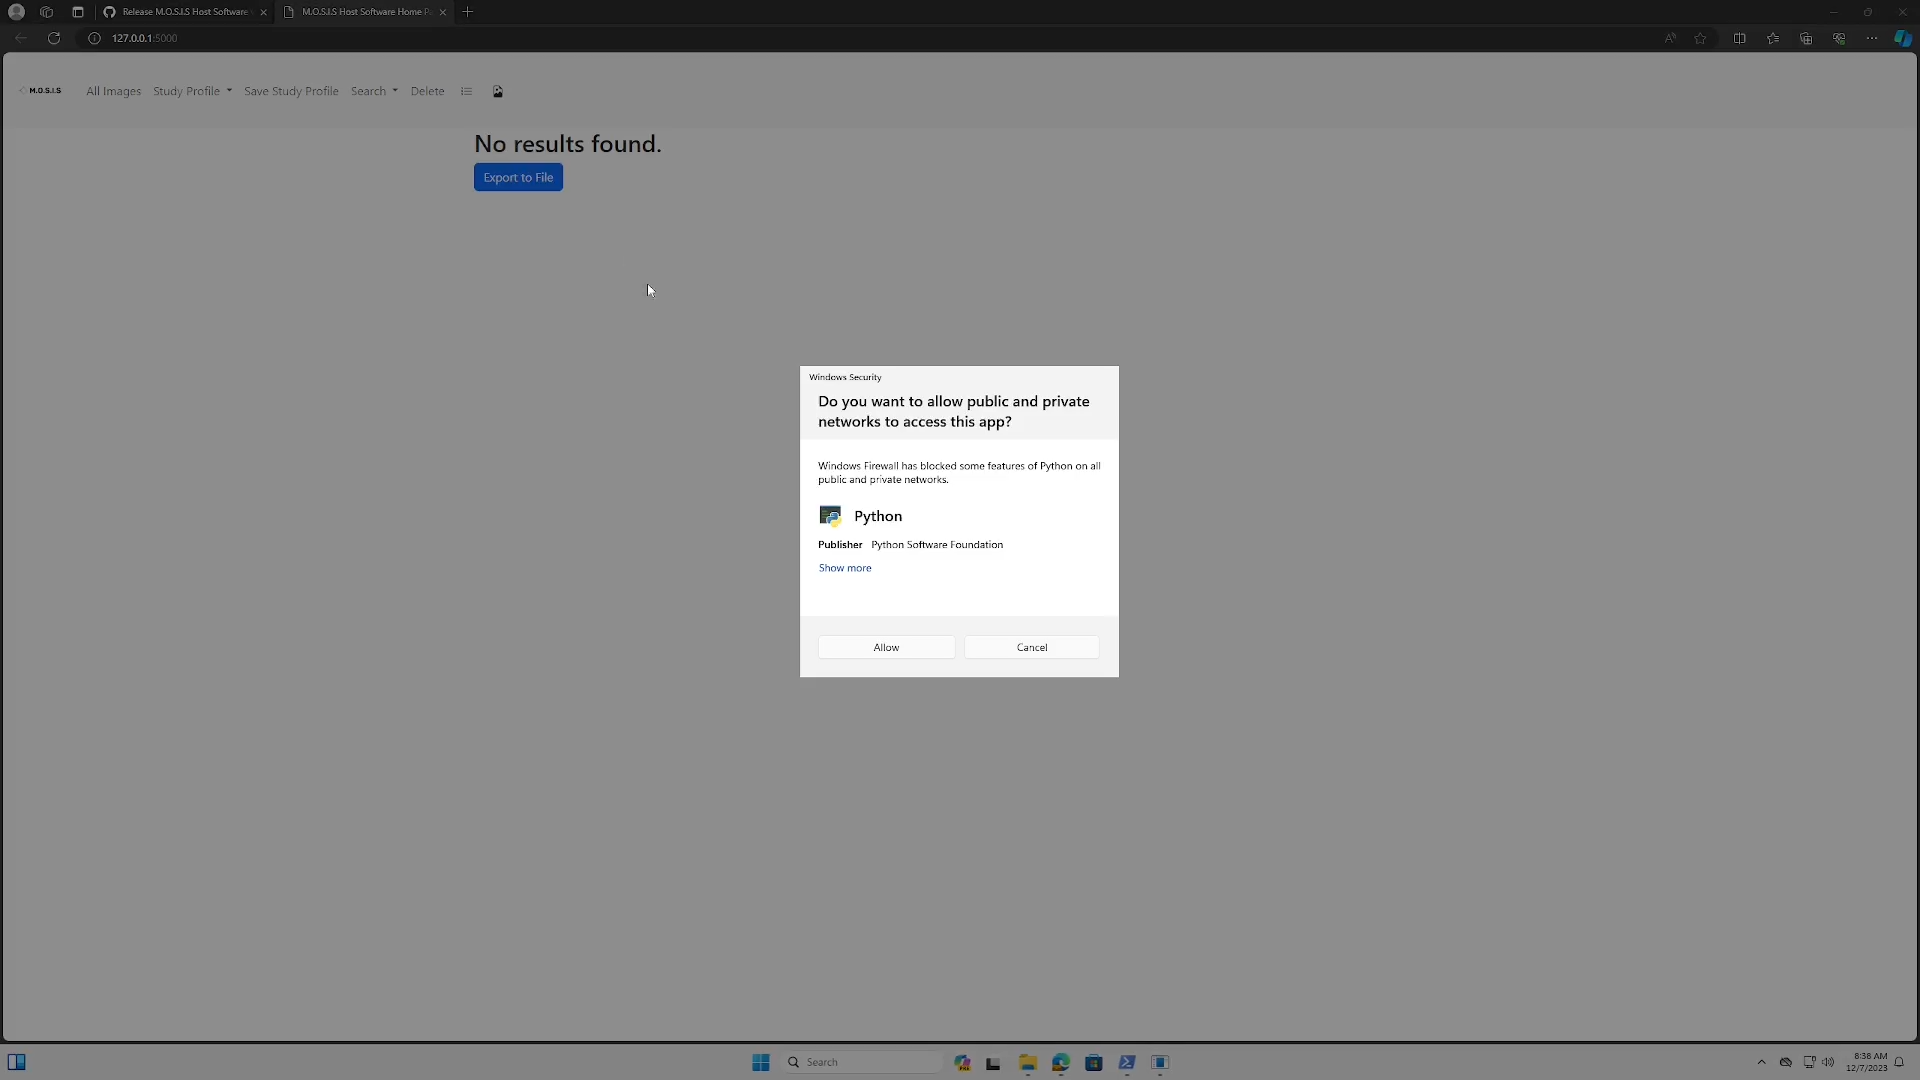
\includegraphics[width=\textwidth]{Figures/Windows-Allow-Python.png}
		      \end{figure}
	\end{enumerate}
	\subsection{Linux}
	\begin{itemize}
		\item Open a web browser
		      \begin{figure}[H]
			      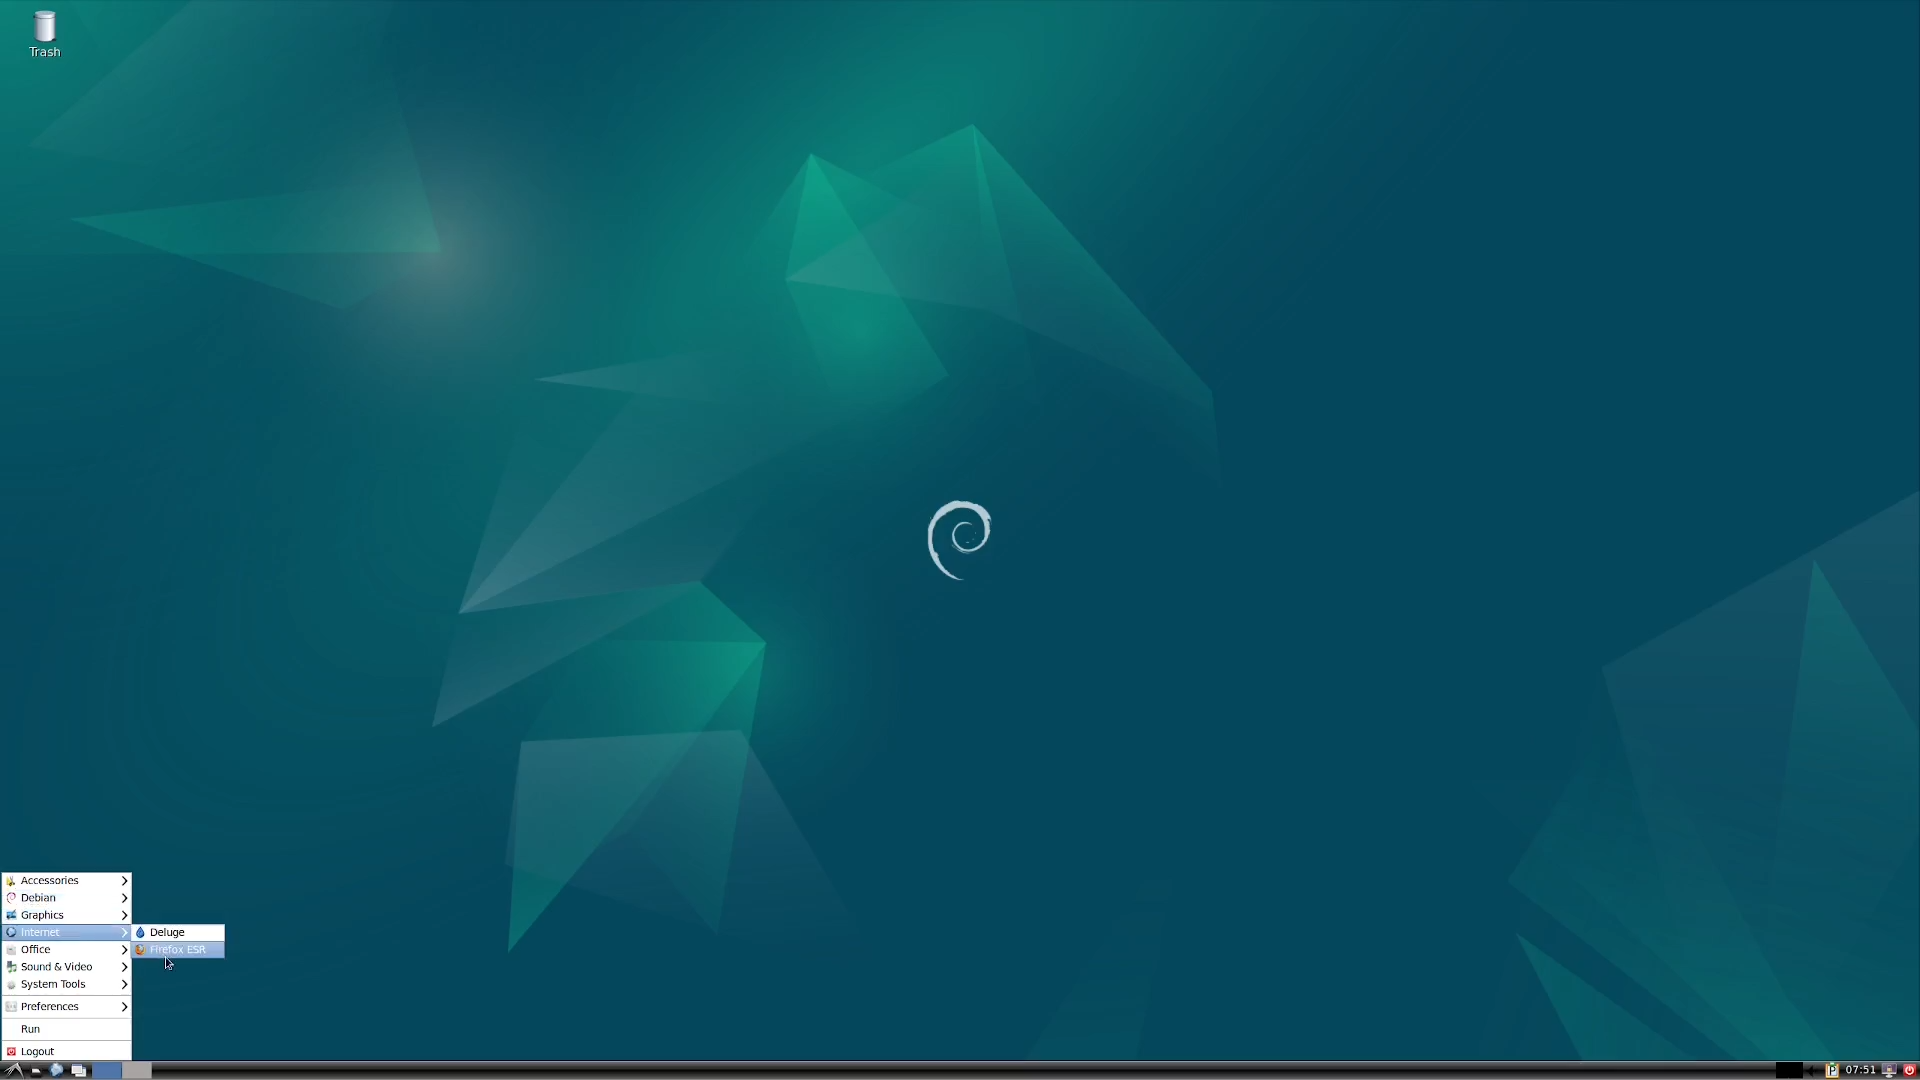
\includegraphics[width=\textwidth]{Figures/Linux-Open-Web-Browser.png}
		      \end{figure}
		\item Go to the repository going to \href{https://github.com/fabiomatos999/M.O.S.I.S}{https://github.com/fabiomatos999/M.O.S.I.S} by clicking here: \href{https://github.com/fabiomatos999/M.O.S.I.S}{link}.
		      \begin{figure}[H]
			      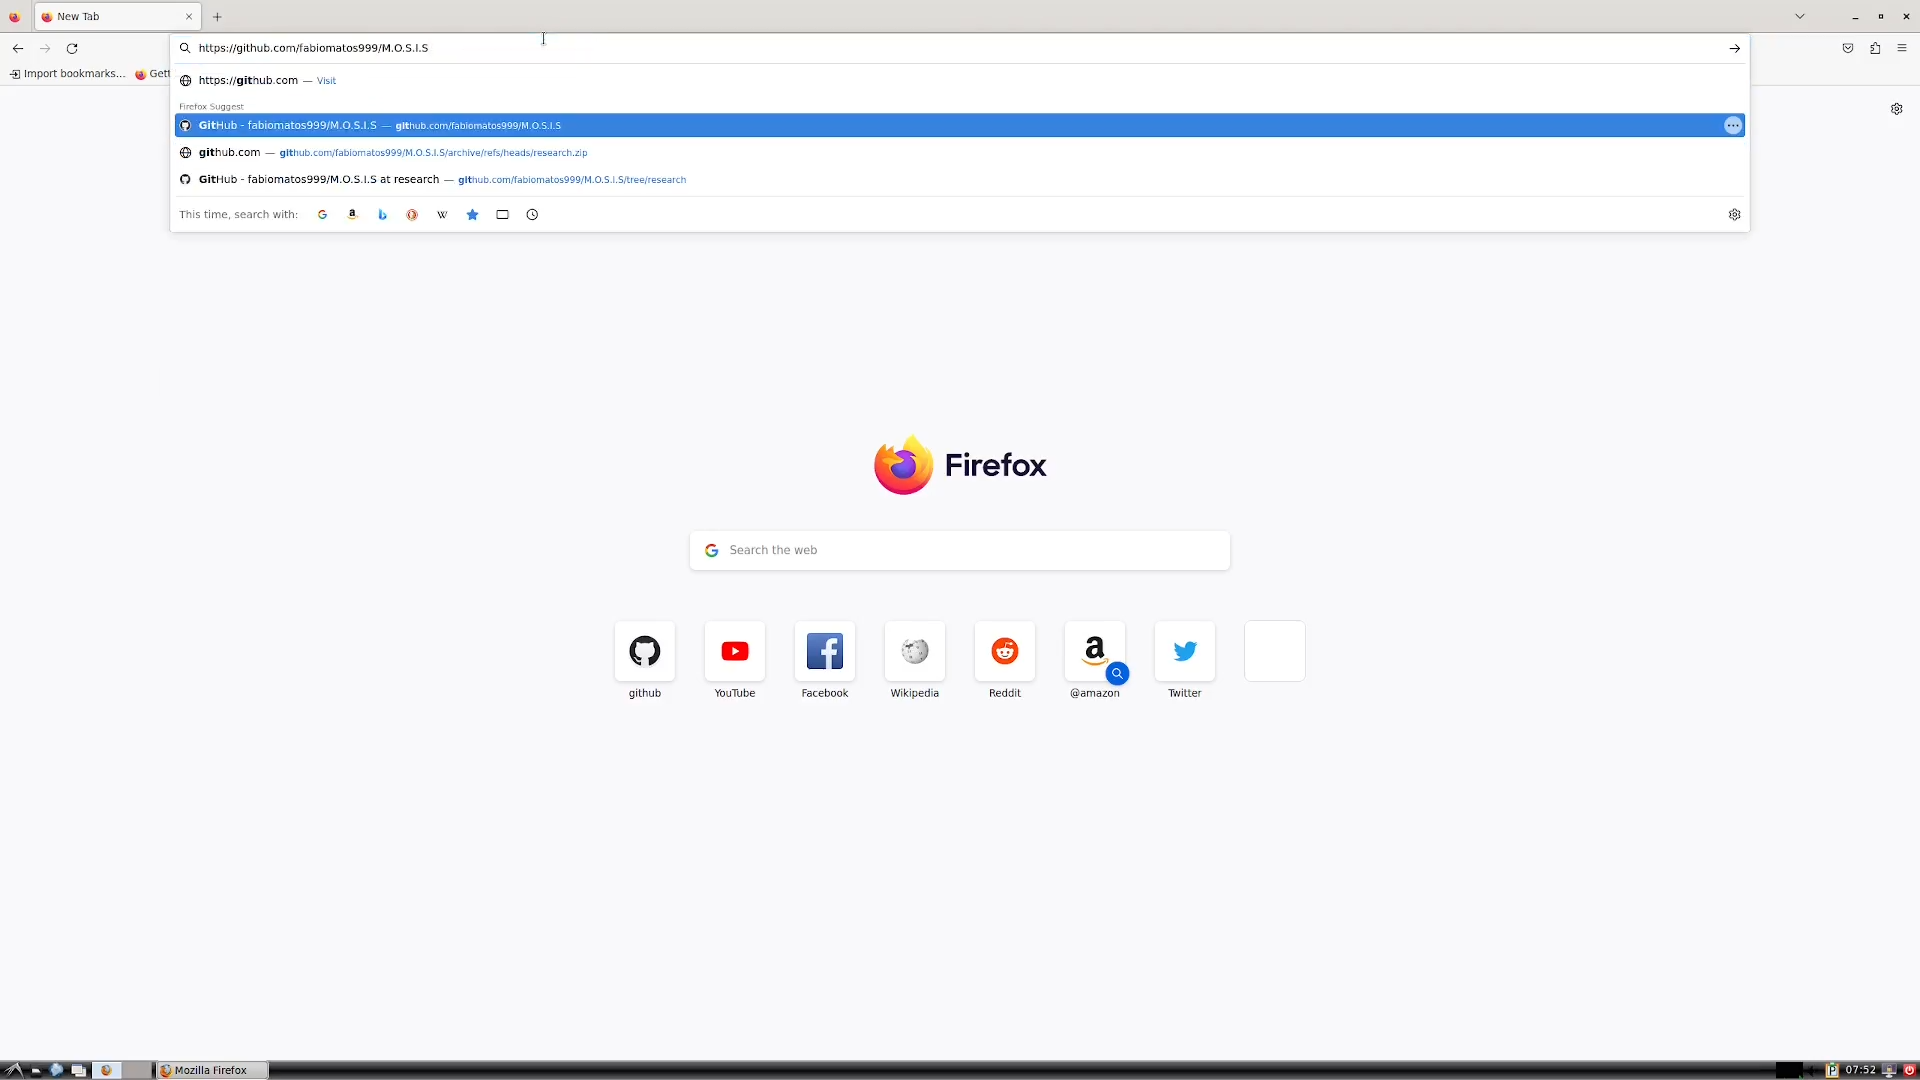
\includegraphics[width=\textwidth]{Figures/Linux-Go-To-Repo.png}
		      \end{figure}
		\item Go the releases page on the Github repository:
		      \begin{figure}[H]
			      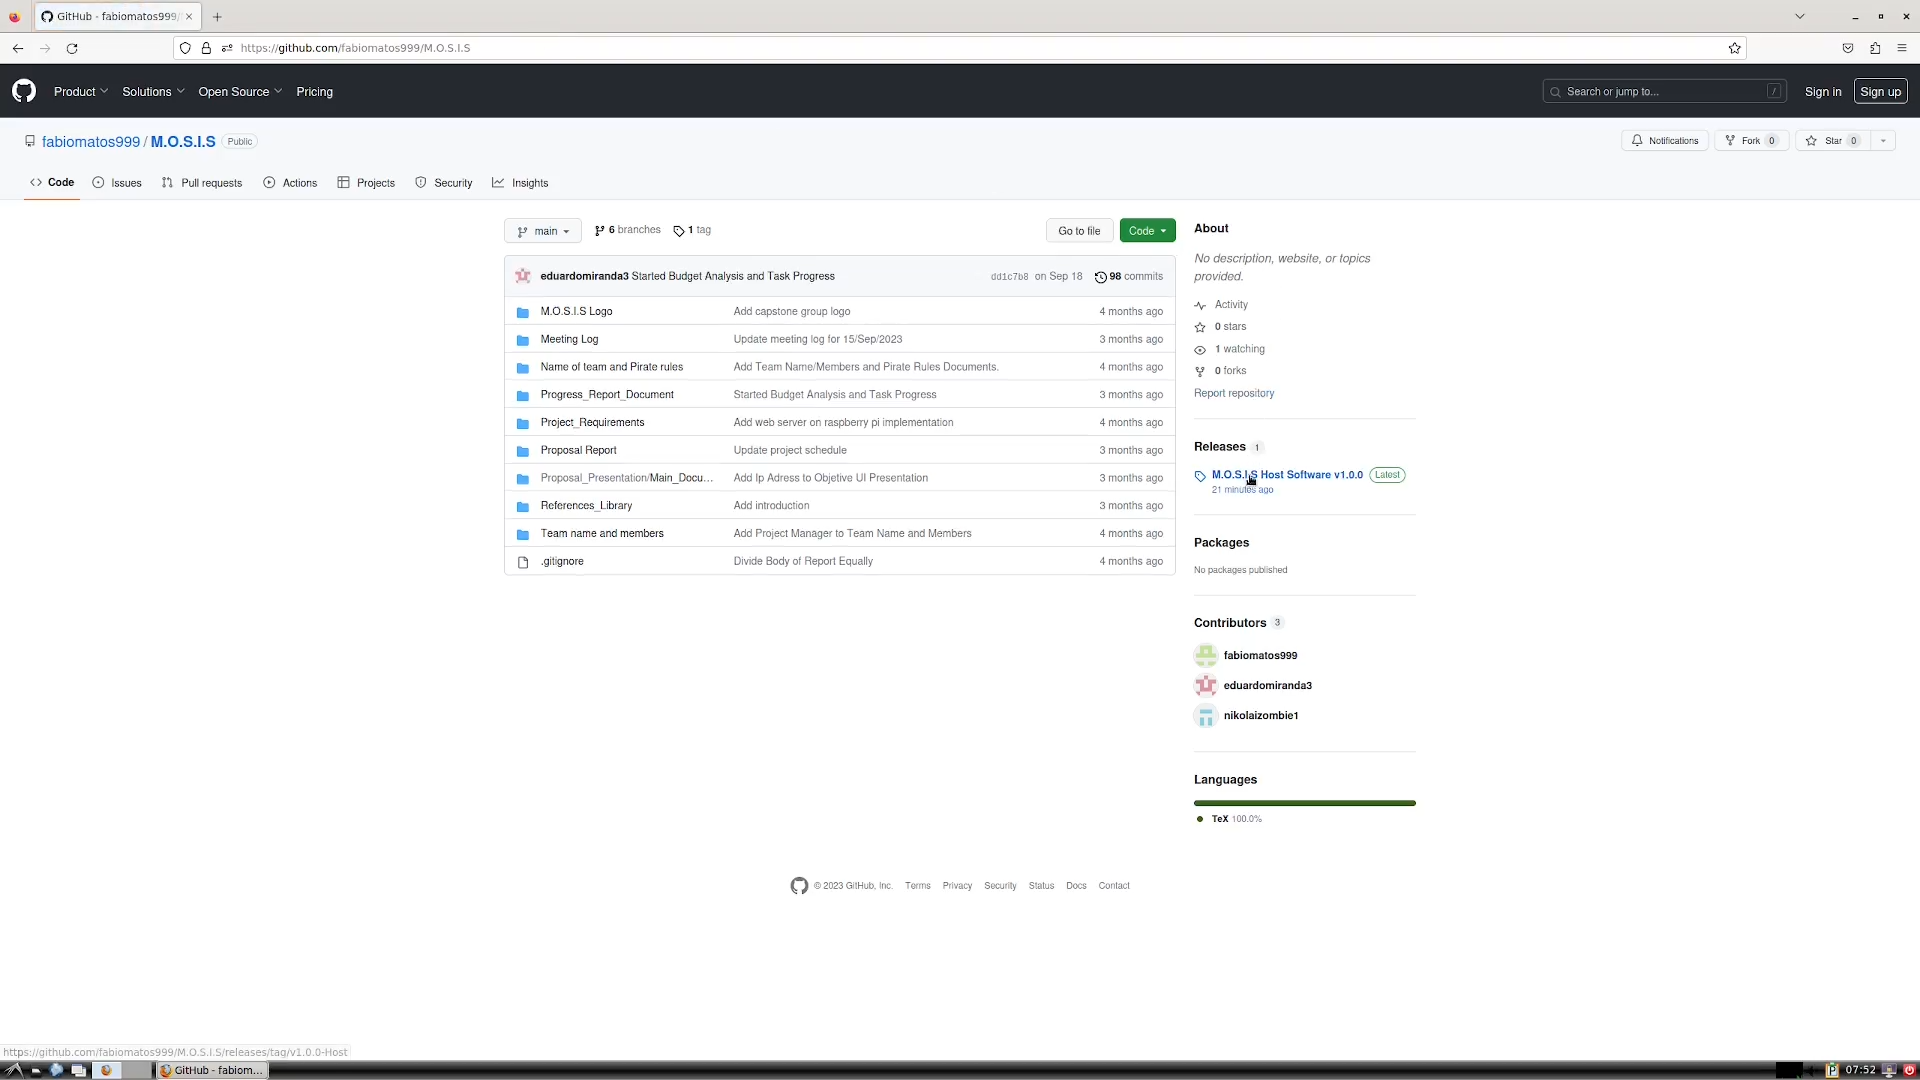
\includegraphics[width=\textwidth]{Figures/Linux-Go-To-Releases.png}
		      \end{figure}
		\item Get Host Software by clicking on the ``M.O.S.I.S\_Host\_Software.zip'' in the latest release (at the time writing v1.0.0)
		      \begin{figure}[H]
			      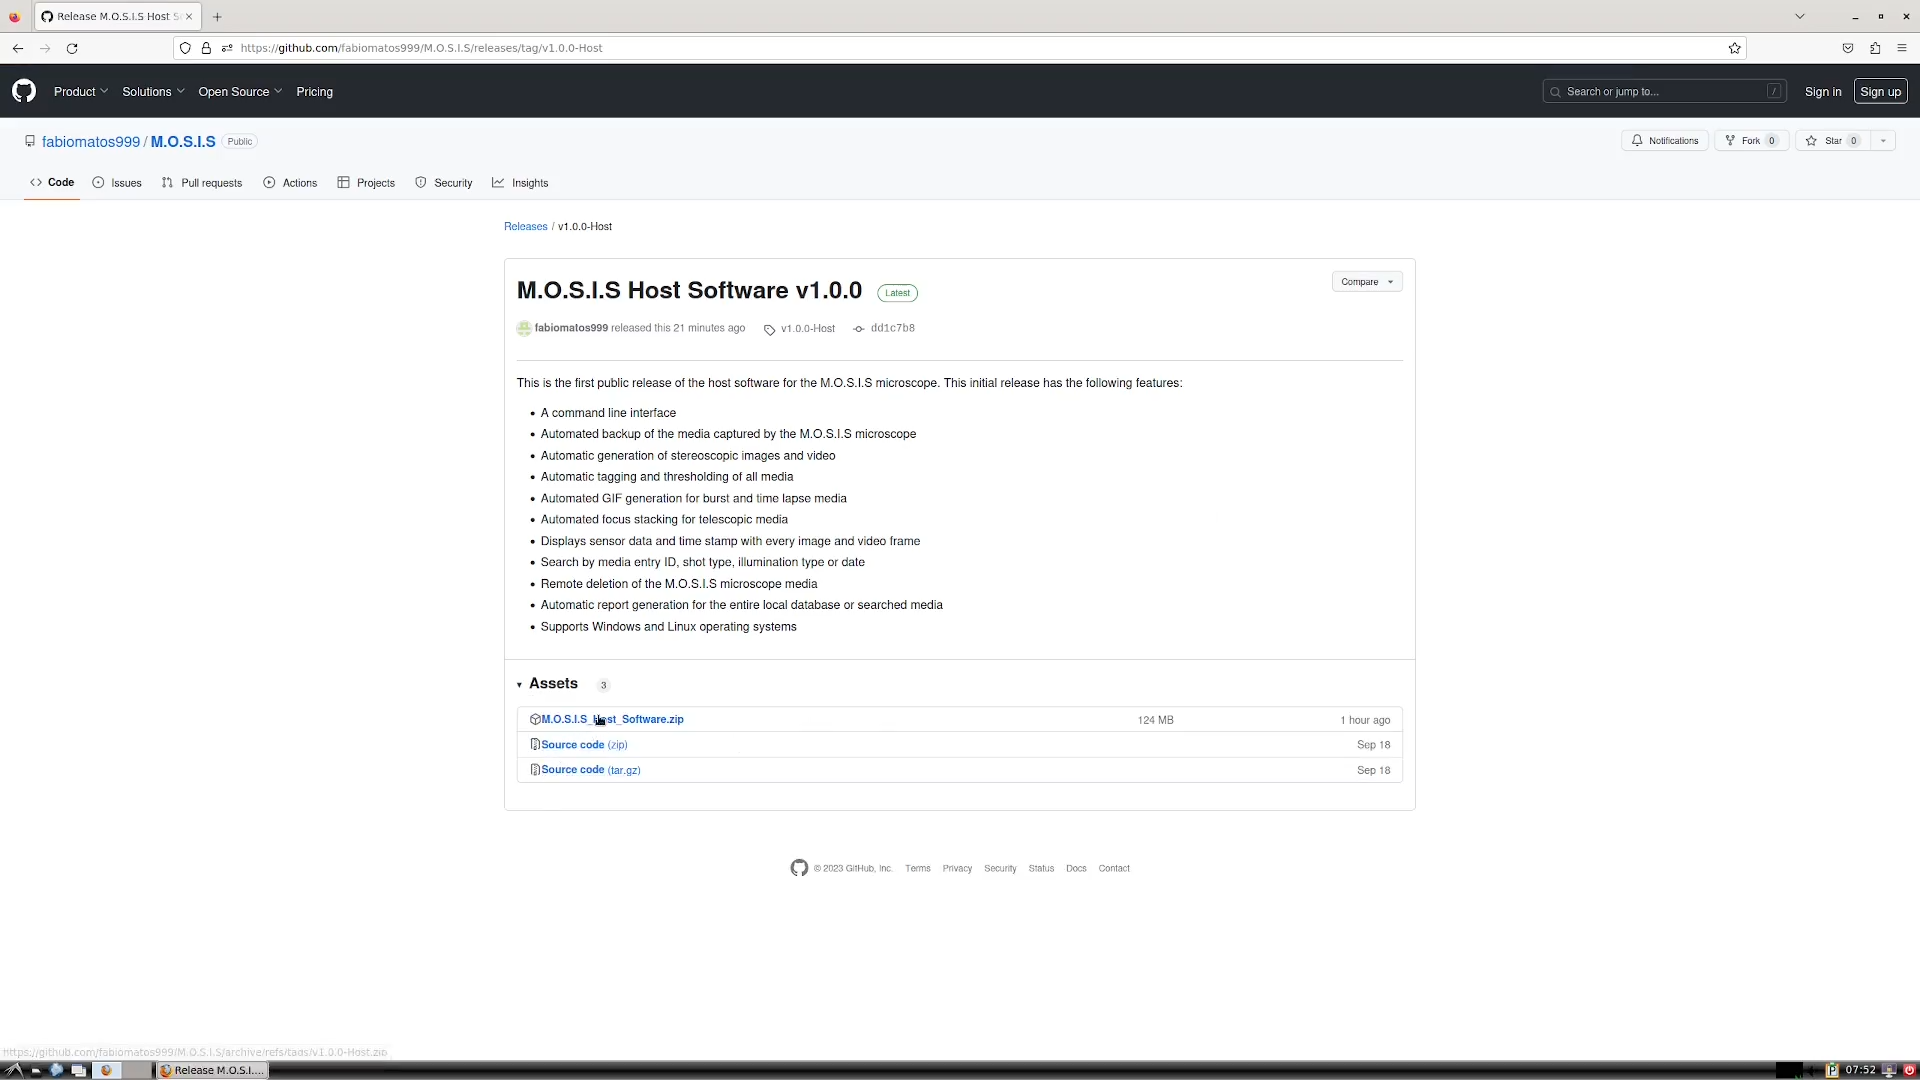
\includegraphics[width=\textwidth]{Figures/Linux-Download-Host-Software-Download.png}
		      \end{figure}
		\item Click on the ``zip'' archive once it has finished downloading
		      \begin{figure}[H]
			      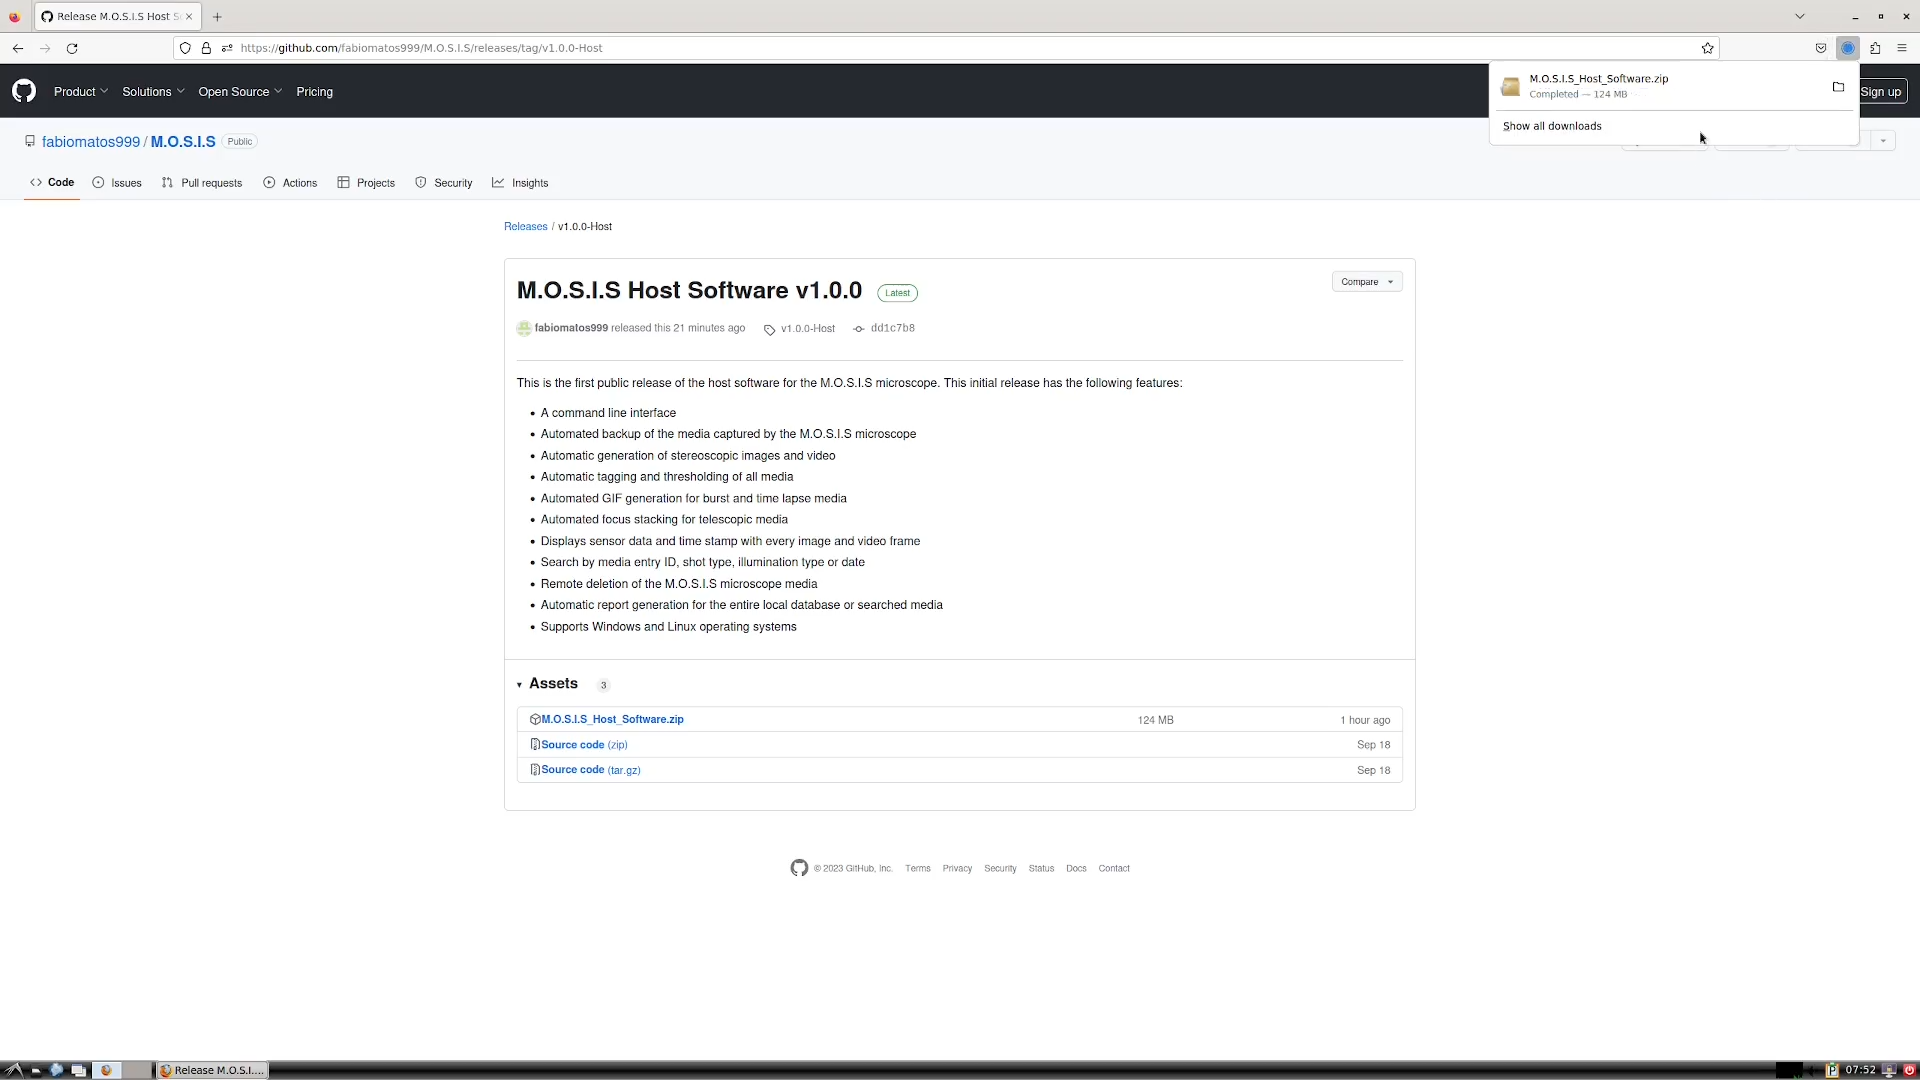
\includegraphics[width=\textwidth]{Figures/Linux-Open-Host-Software-Archive.png}
		      \end{figure}
		\item Follow the next steps to extract the ``zip'' archive into the downloads folder.
		      \begin{figure}[H]
			      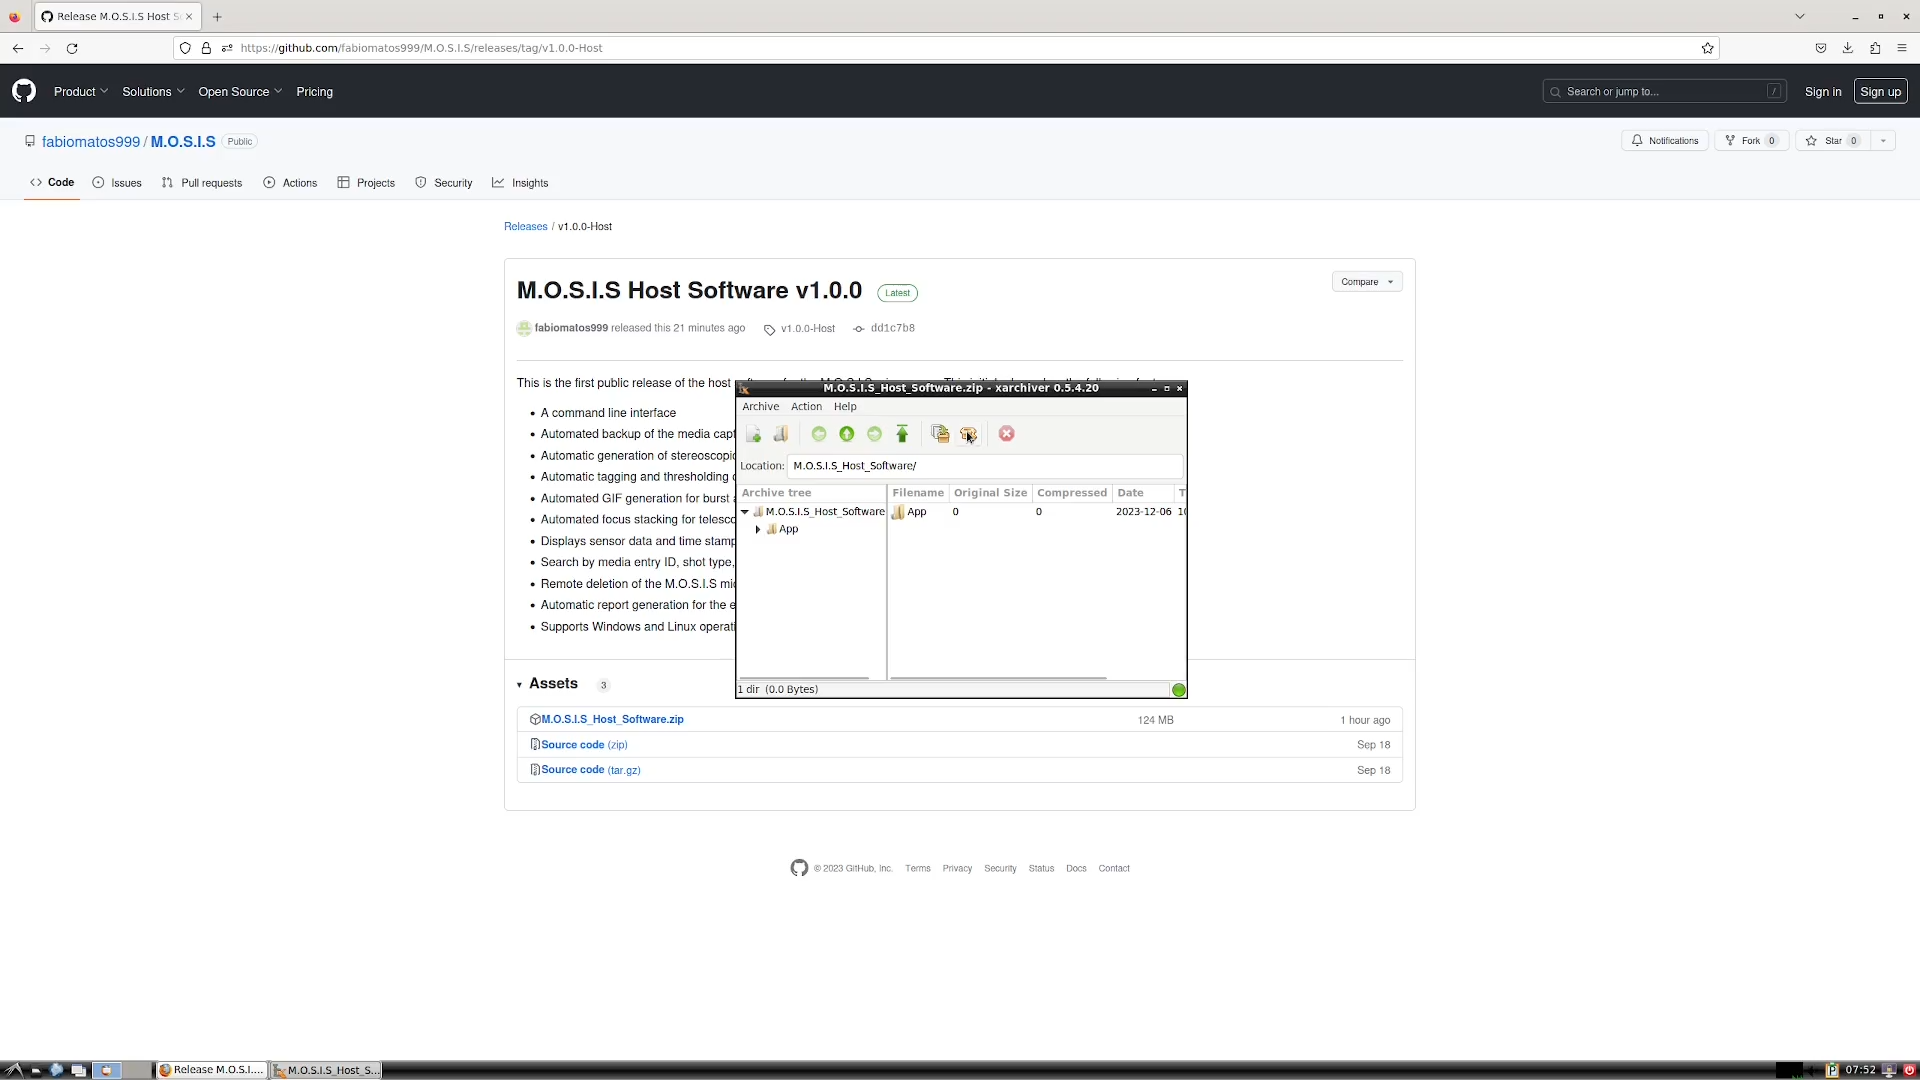
\includegraphics[width=\textwidth]{Figures/Linix-Extract-Archive.png}
		      \end{figure}
		      \begin{figure}[H]
			      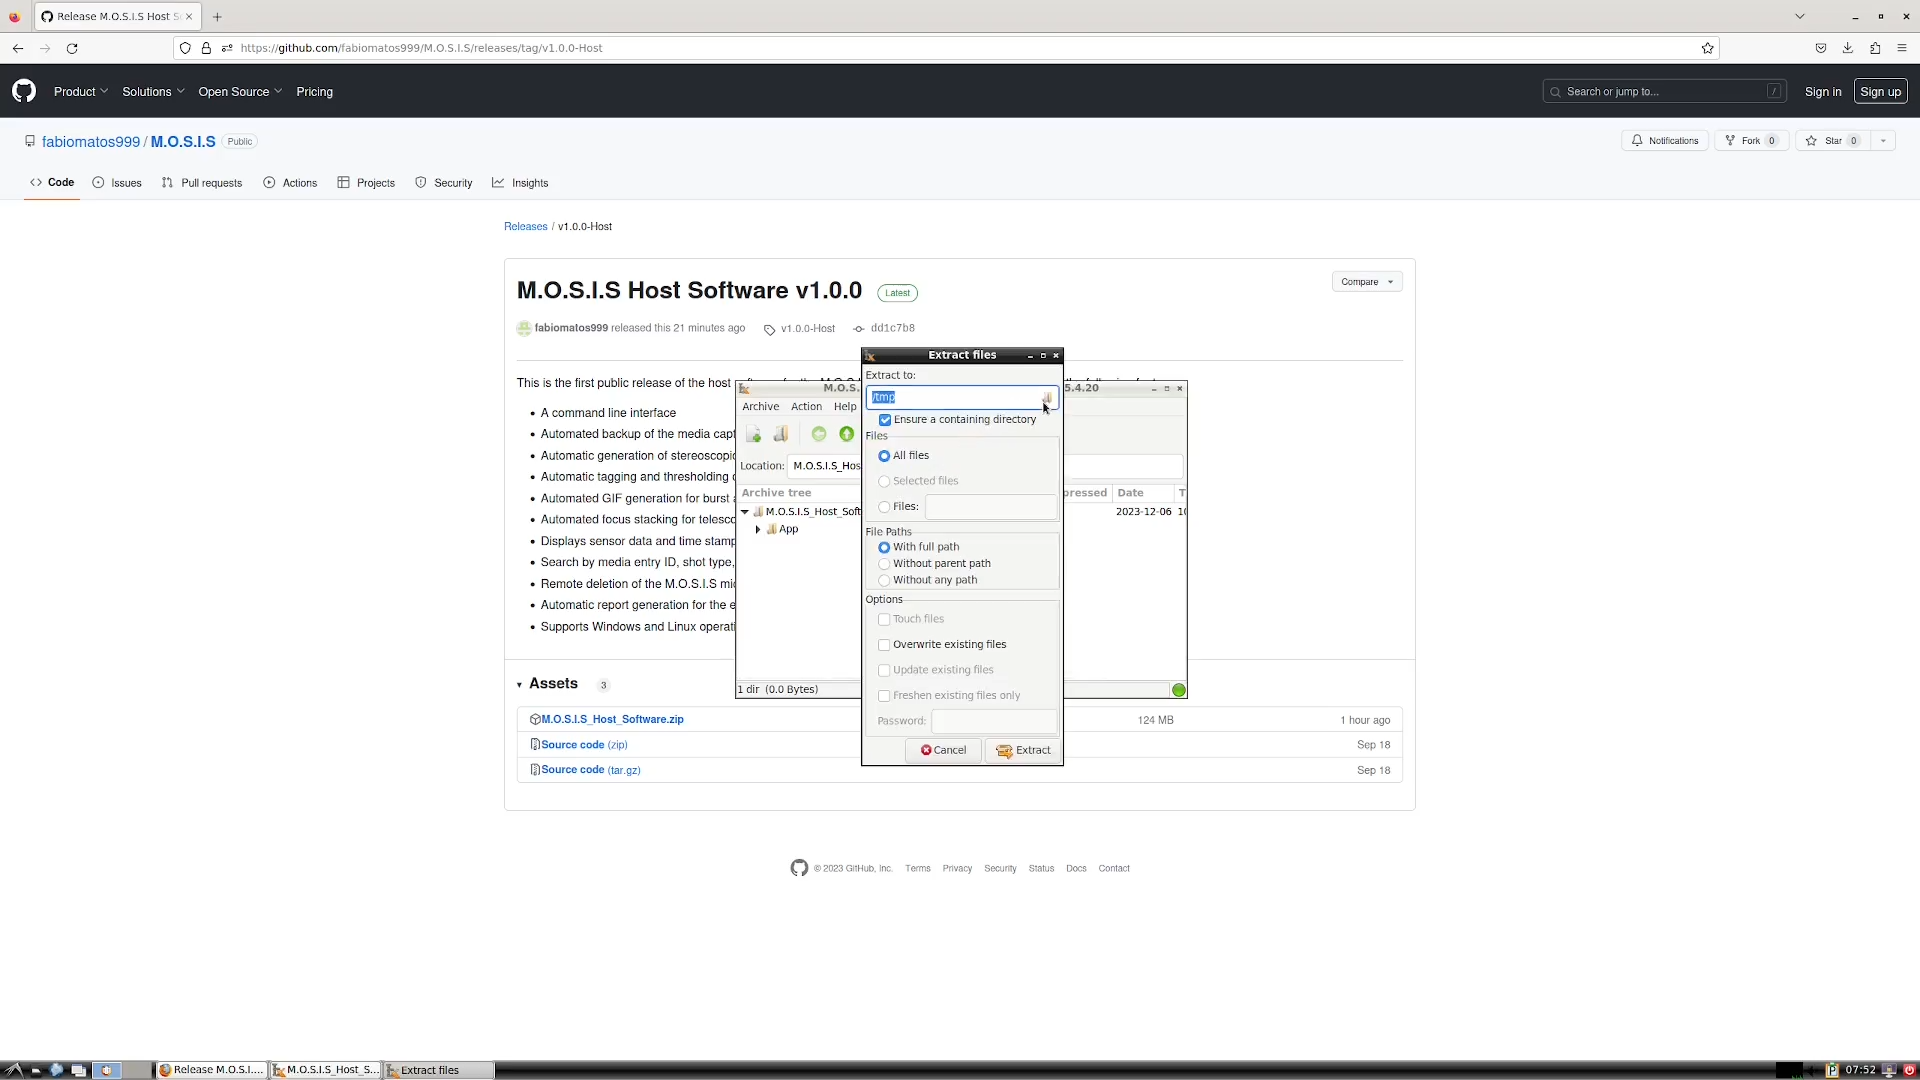
\includegraphics[width=\textwidth]{Figures/Linix-Extract-Archive-2.png}
		      \end{figure}
		      \begin{figure}[H]
			      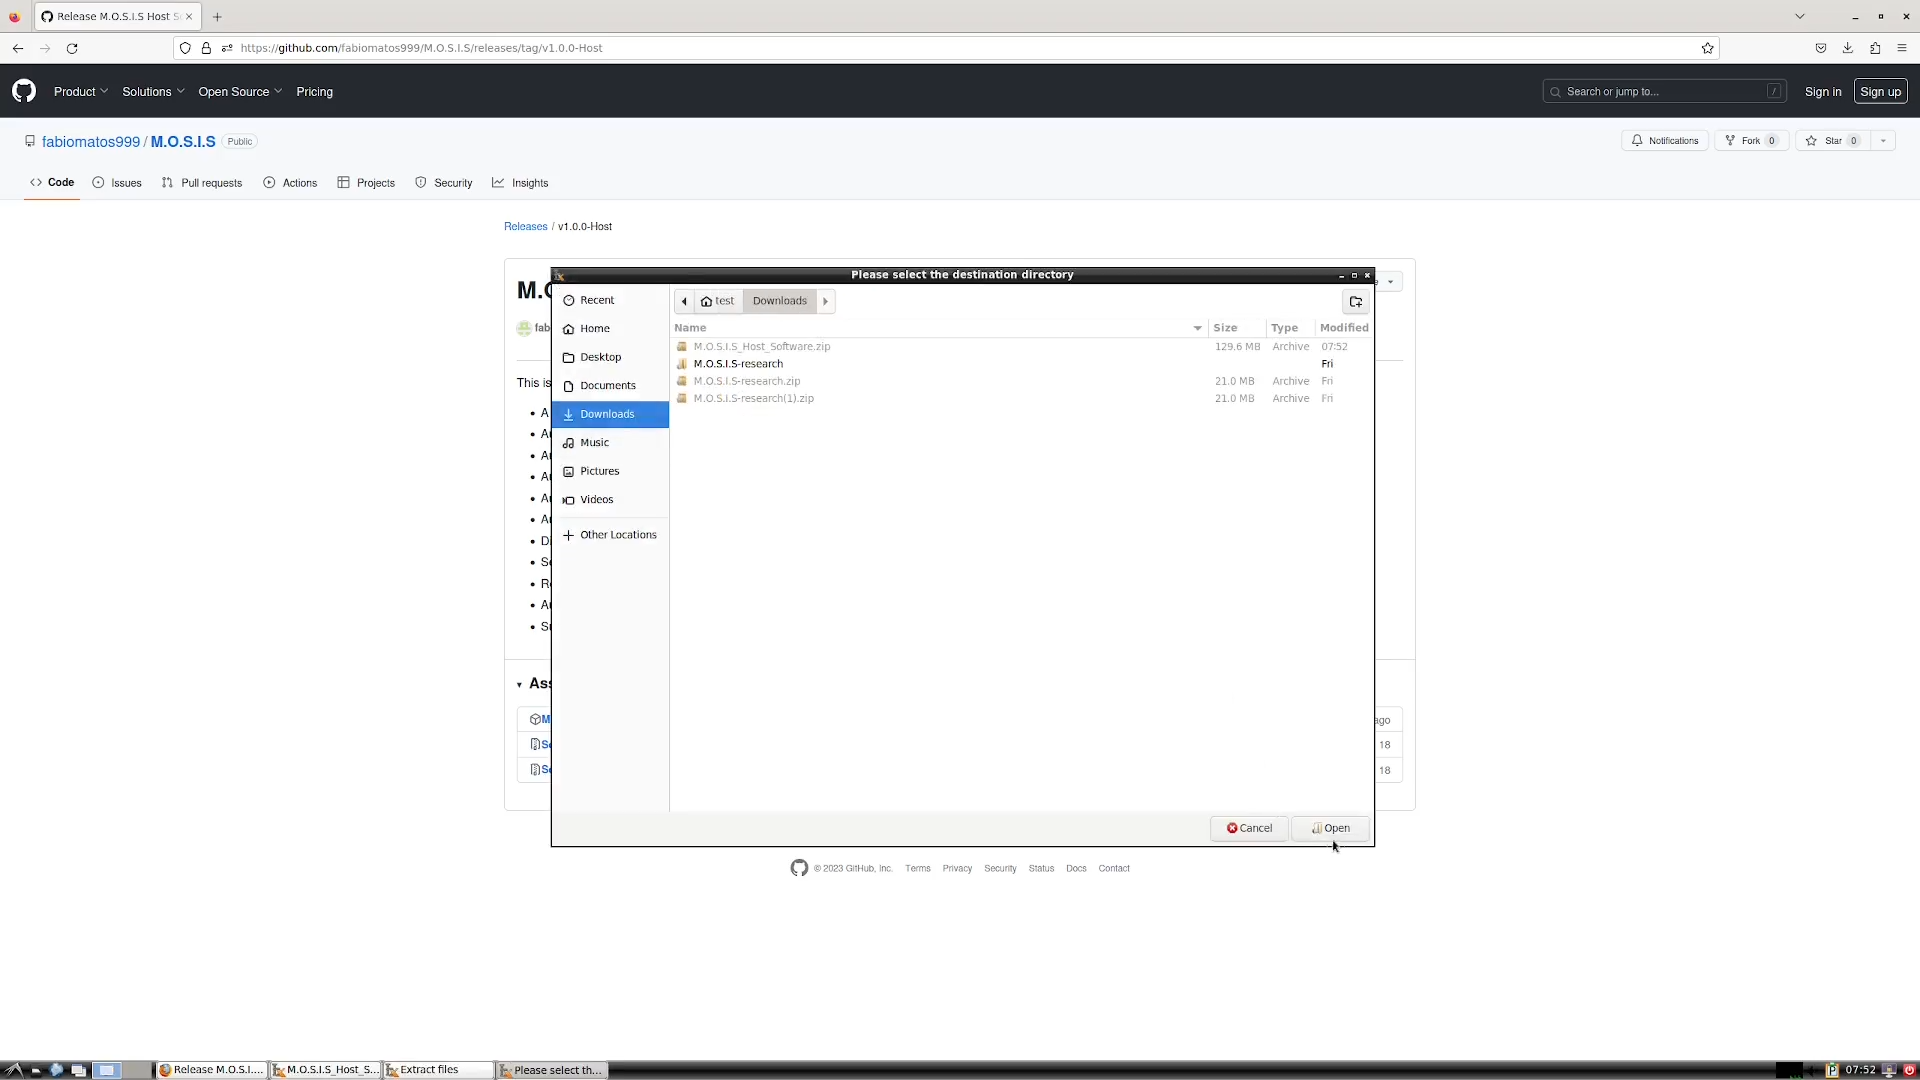
\includegraphics[width=\textwidth]{Figures/Linix-Extract-Archive-3.png}
		      \end{figure}
		\item Open a terminal
		      \begin{figure}[H]
			      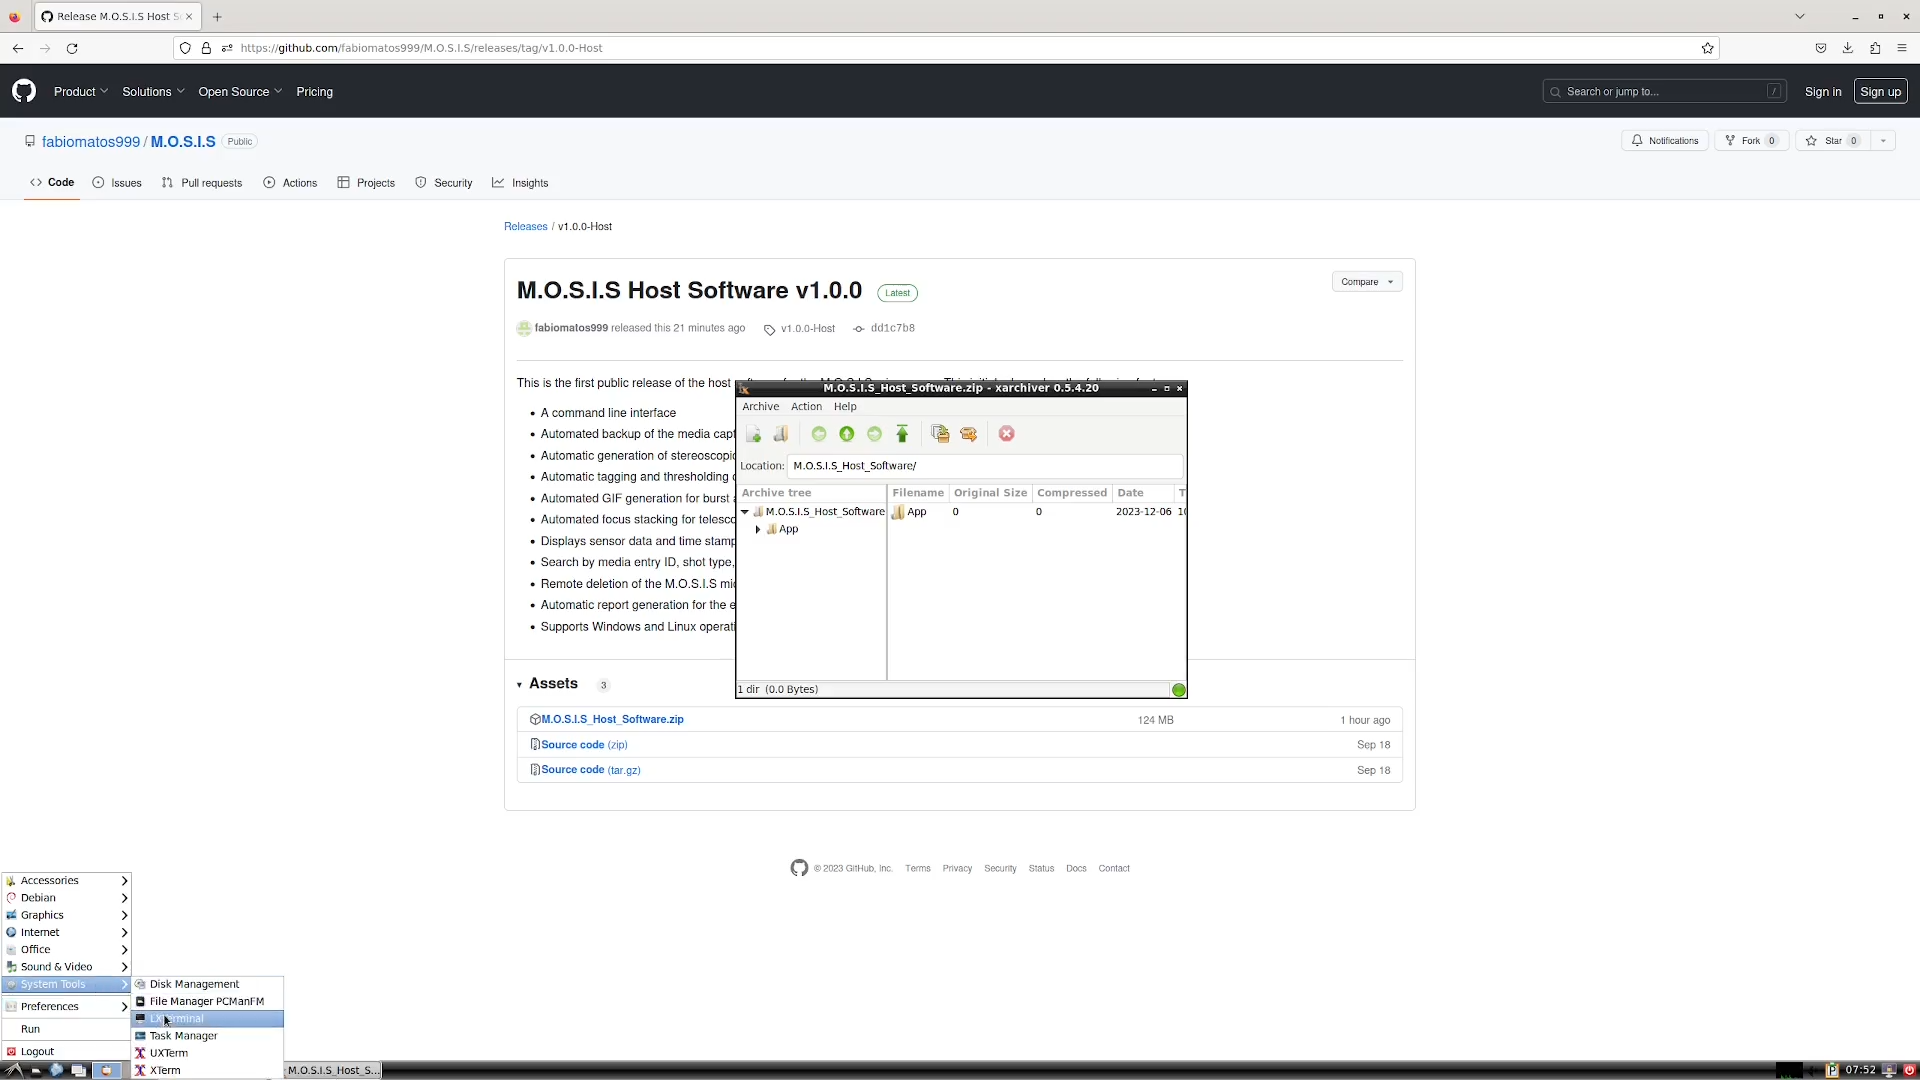
\includegraphics[width=\textwidth]{Figures/Linux-Open-terminal.png}
		      \end{figure}
		\item Change directory to where the host software was extracted
		      \begin{minted}{bash}
                        cd Downloads/M.O.S.I.S_Host_Software/App
                      \end{minted}
		      \begin{figure}[H]
			      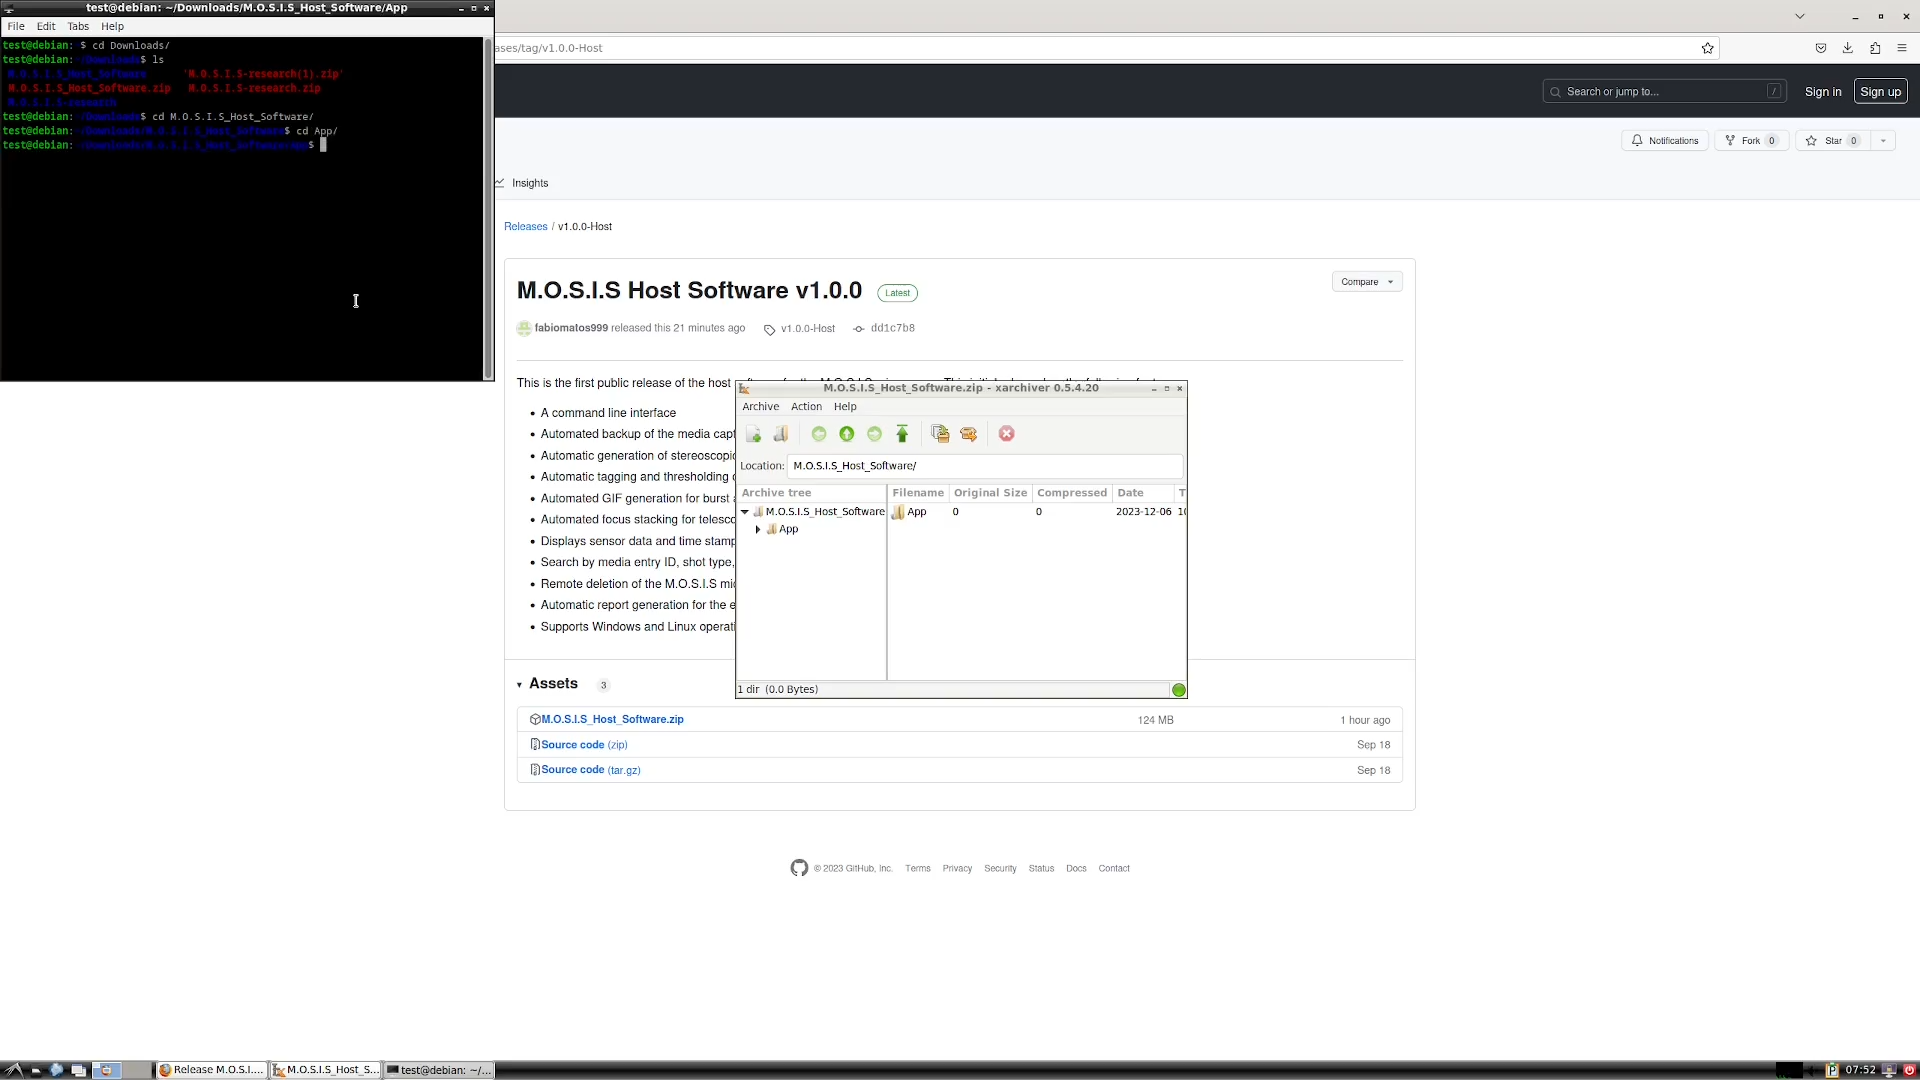
\includegraphics[width=\textwidth]{Figures/Linux-cd-Host-Software.png}
		      \end{figure}
		\item Launch the host software by typing the following in the terminal and then pressing enter
		      \begin{minted}{bash}
                       ./start_app.bash -n 
                      \end{minted}
		      \begin{figure}[H]
			      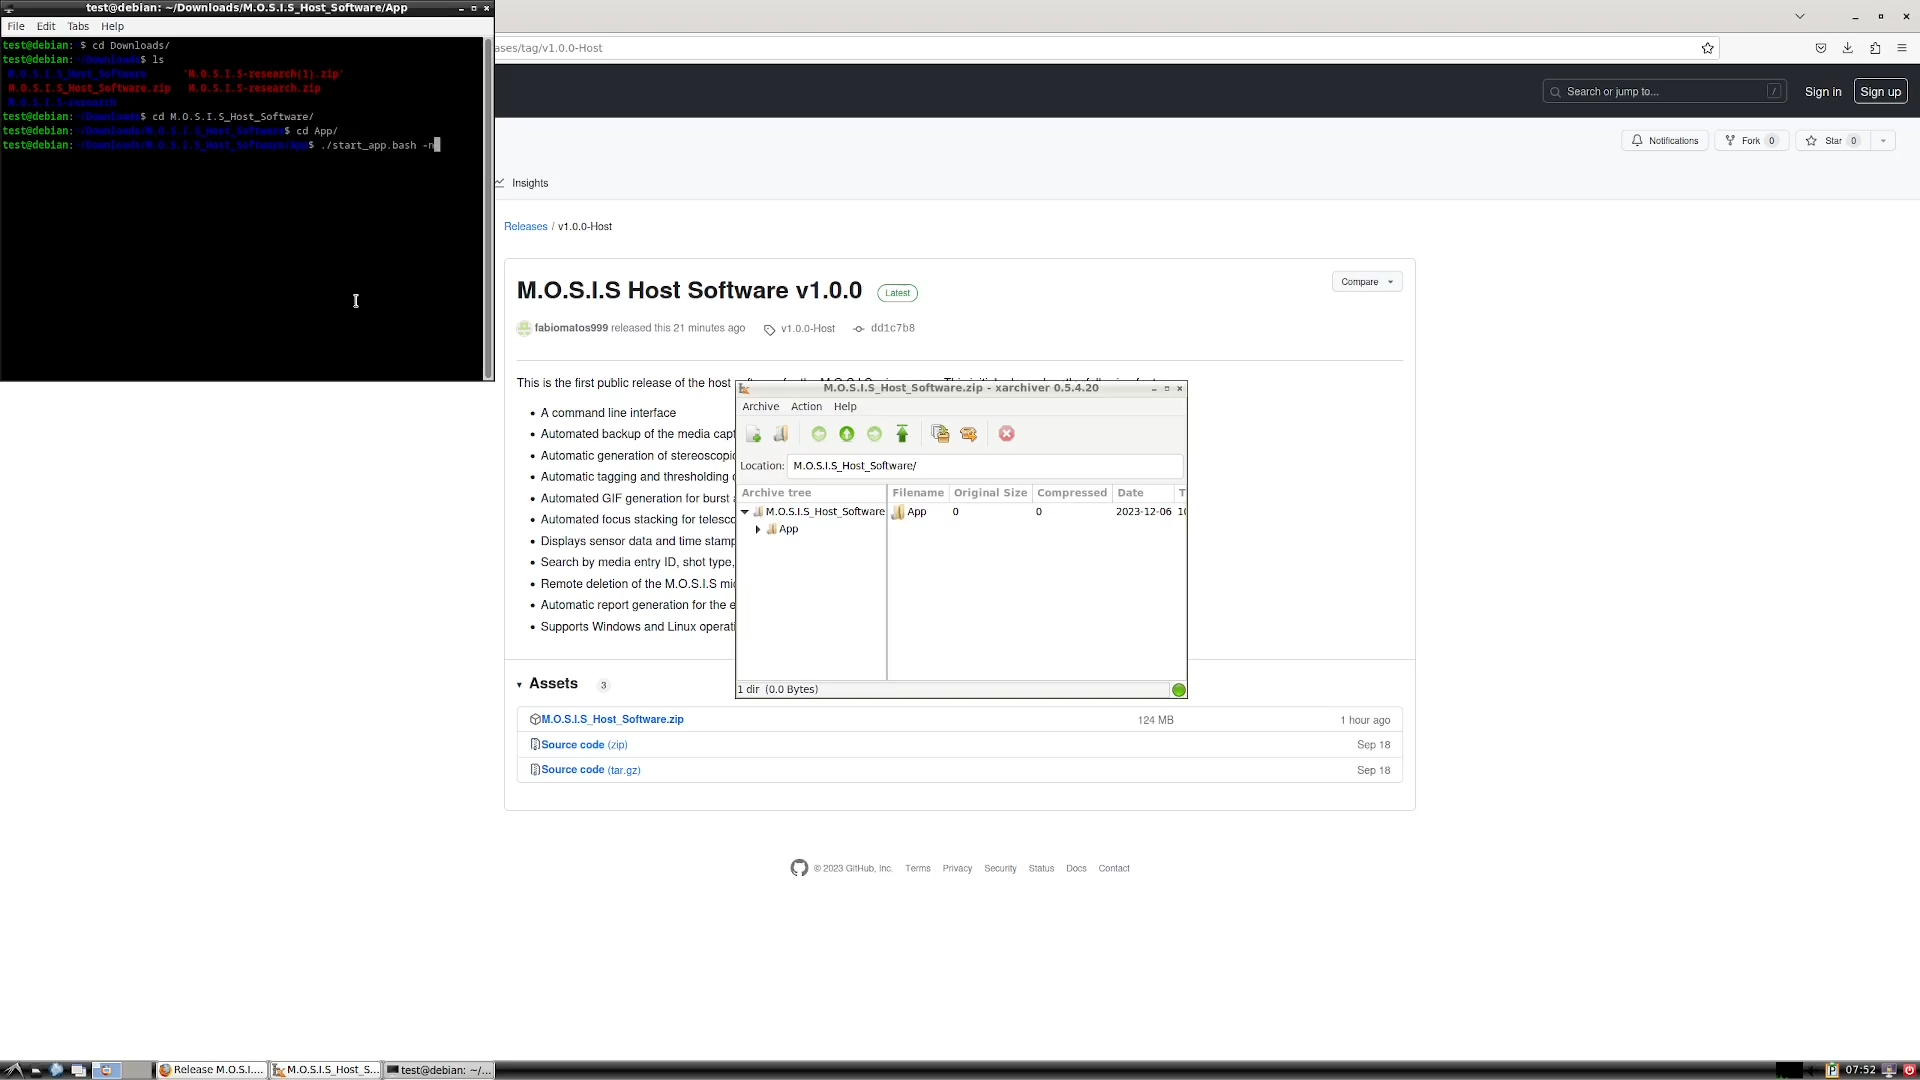
\includegraphics[width=\textwidth]{Figures/Linux-Start-Host-Software-First-Time.png}
		      \end{figure}
		\item It should ask you for your password in order to start the installer, write your password and press enter
		      \begin{figure}[H]
			      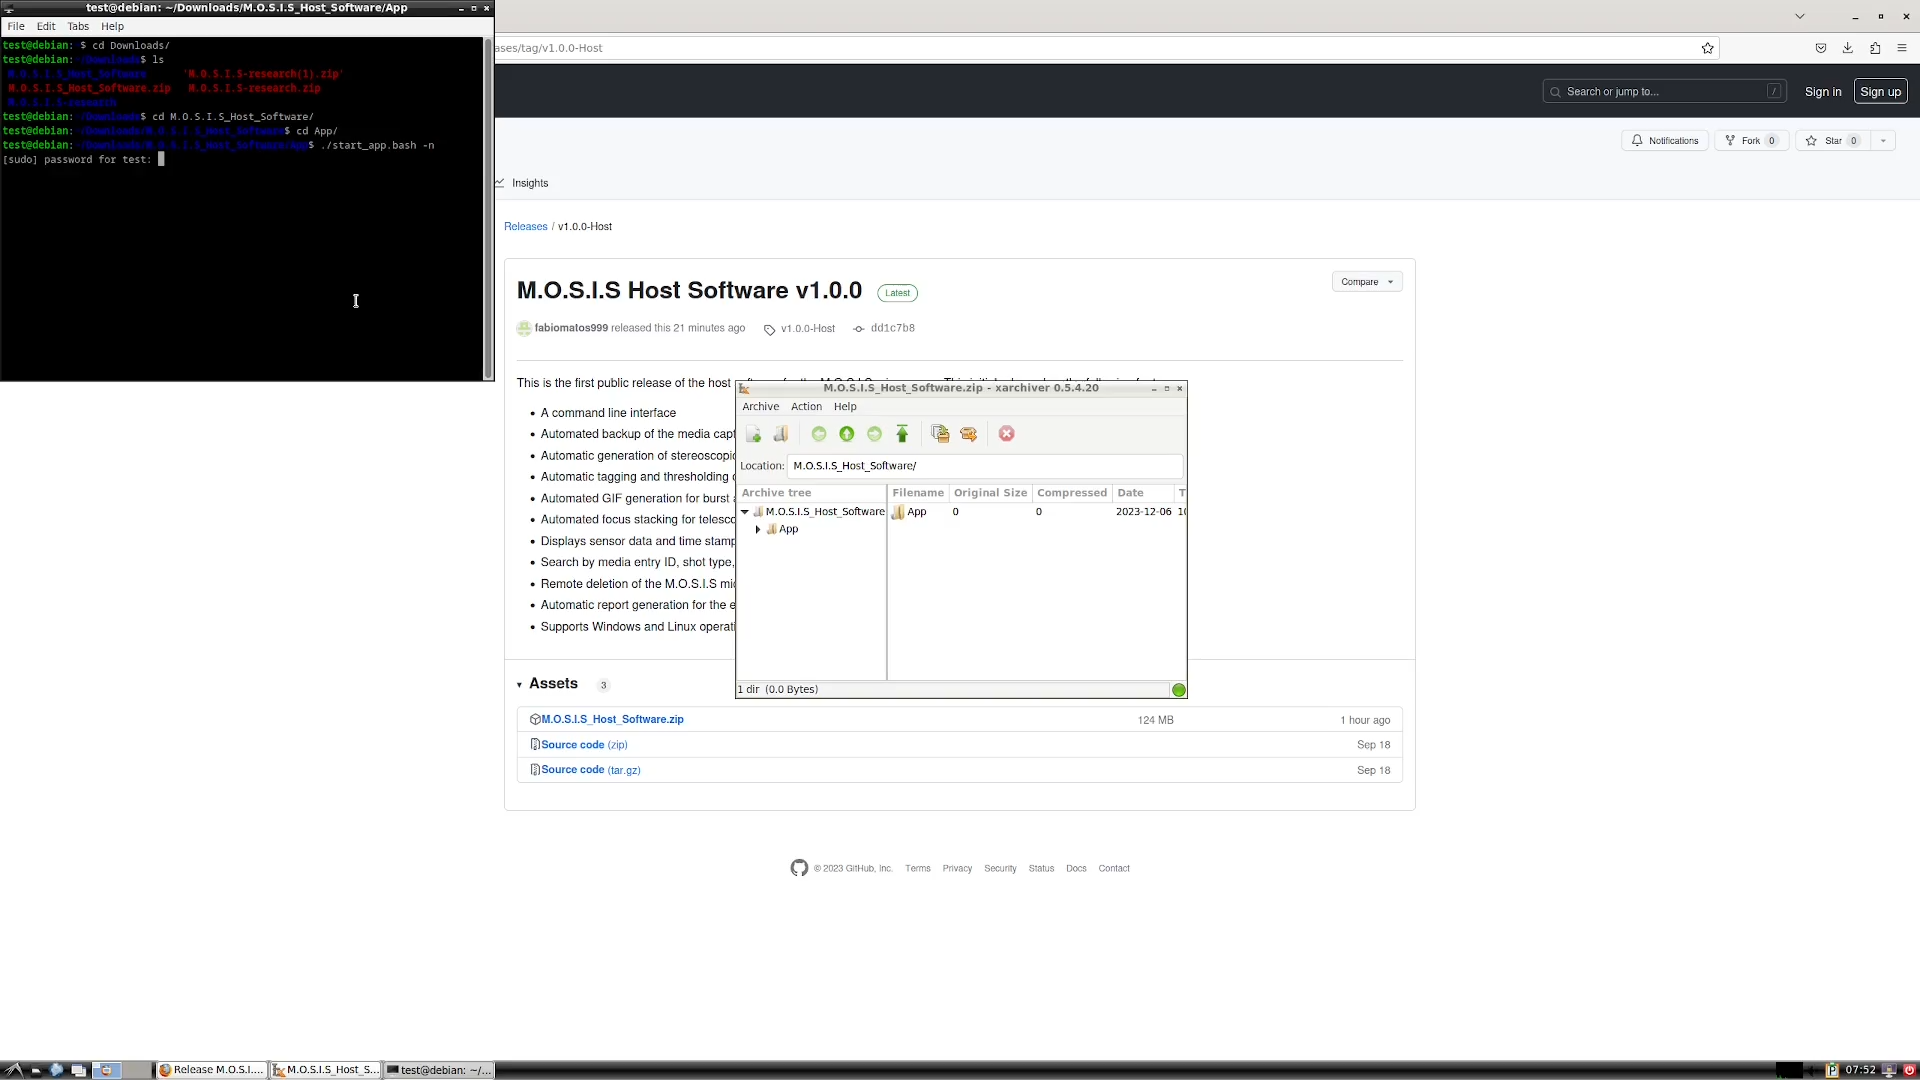
\includegraphics[width=\textwidth]{Figures/Linux-Sudo-Prompt.png}
		      \end{figure}
		\item The rest of the installation will proceed automatically, please wait until it has finished.
		      \begin{figure}[H]
			      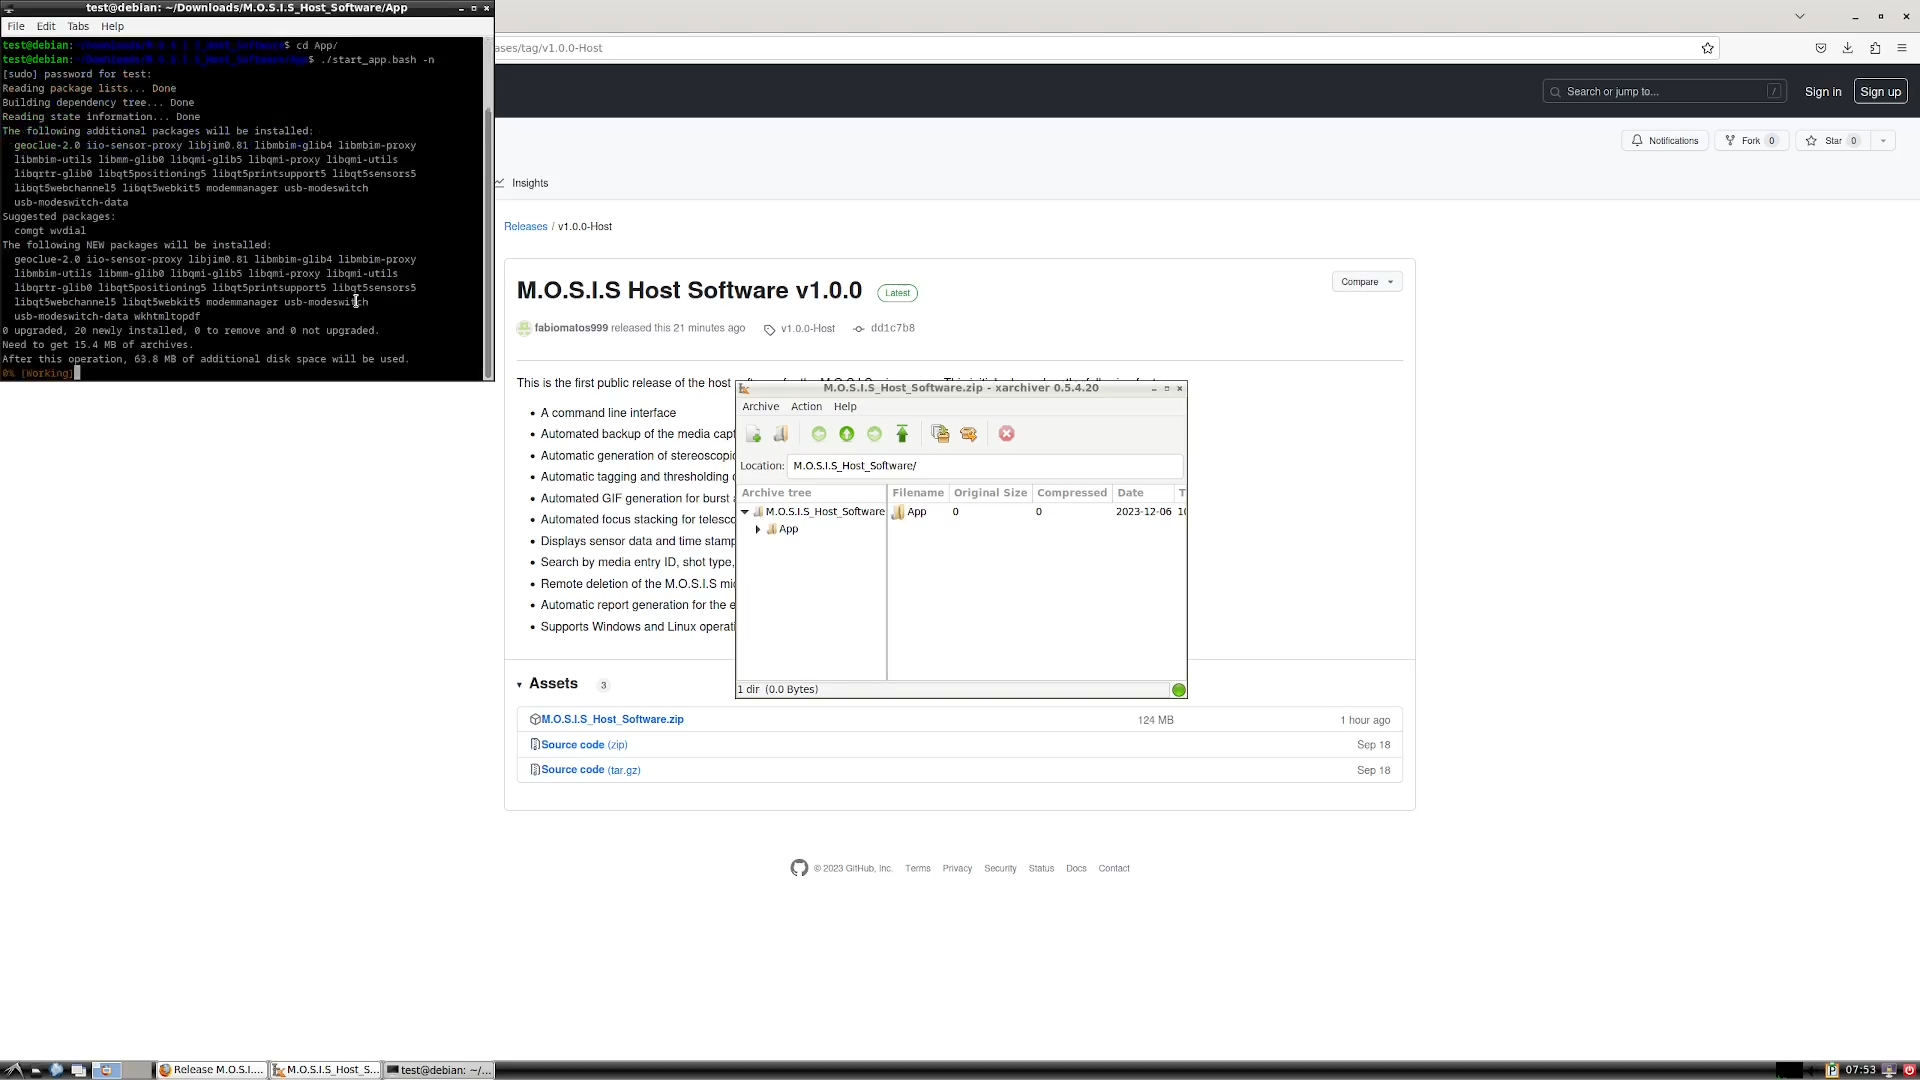
\includegraphics[width=\textwidth]{Figures/Linux-Host-Software-Installer.png}
		      \end{figure}
		\item You will know the installer had finished when a web browser should open with the host software. If it says that the connection failed, refresh the web page.
		      \begin{figure}[H]
			      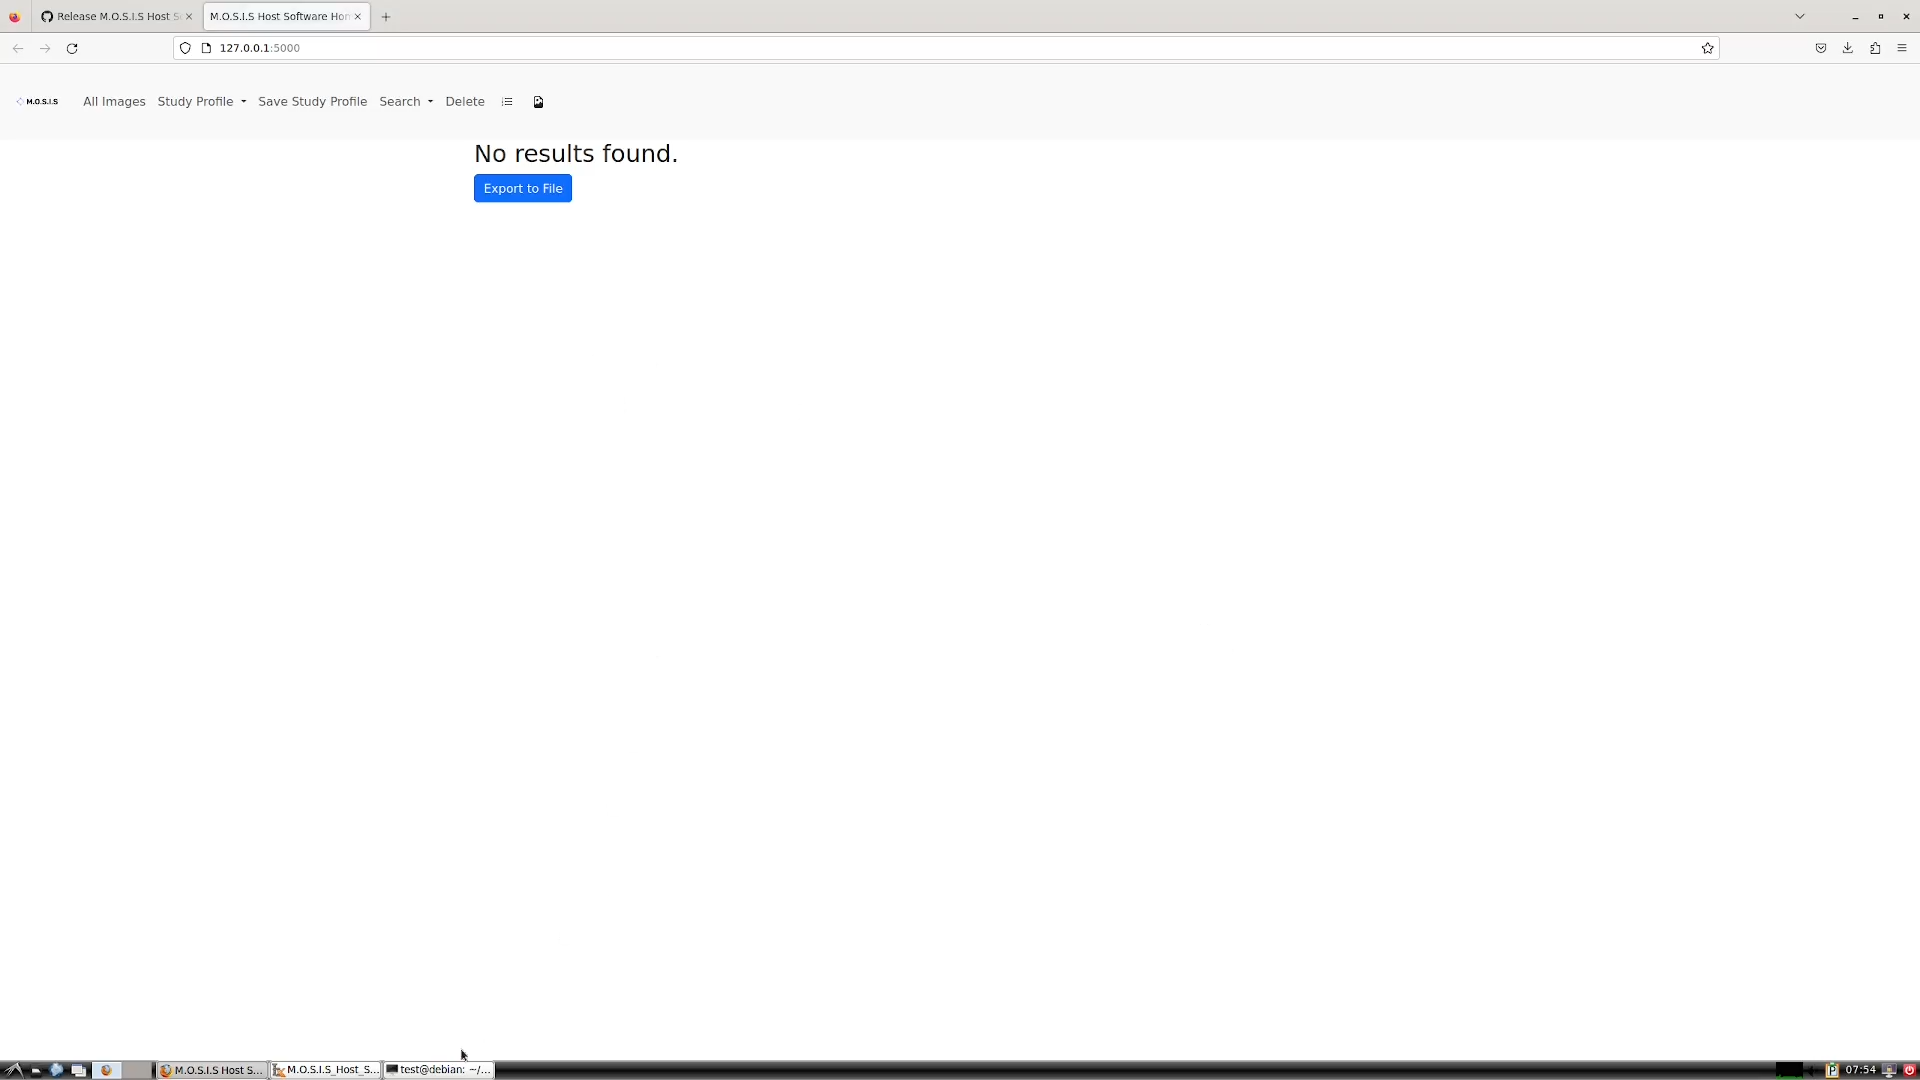
\includegraphics[width=\textwidth]{Figures/Linux-Host-Software-Install-Finish.png}
		      \end{figure}
	\end{itemize}
	\section{Start Host Software}
	\subsection{Windows}
	\begin{enumerate}
		\item Open Powershell clicking on the ``open'' button
		      \begin{figure}[H]
			      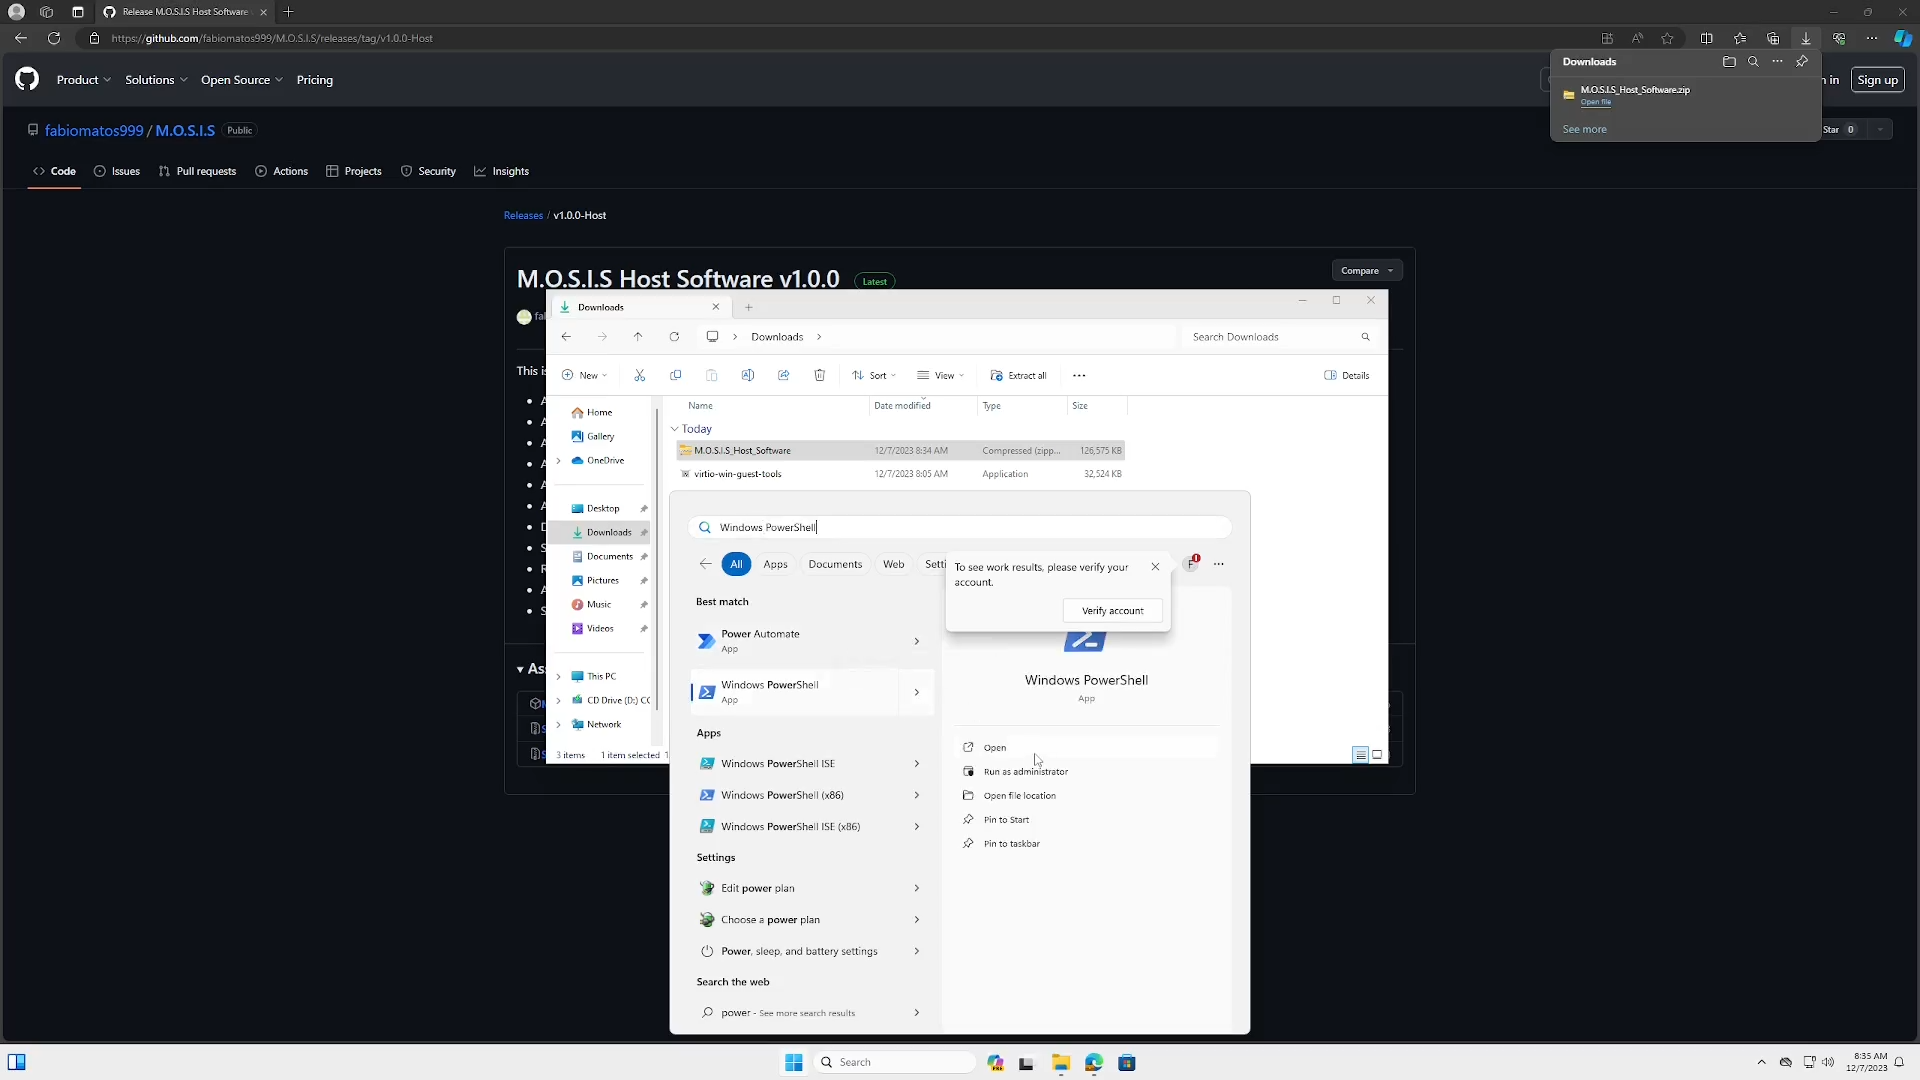
\includegraphics[width=\textwidth]{Figures/Windows-Open-Powershell.png}
		      \end{figure}
		\item Now change directory into where you extracted the host software. Assuming you extracted the host software zip in the Downloads folder, type the following command into the Powershell and press enter.
		      \small\begin{minted}[breaksymbolleft=]{ps1}
    cd .\Downloads\M.O.S.I.S_Host_Software\M.O.S.I.S_Host_Software\App\
  \end{minted}
		      \normalsize
		      \begin{figure}[H]
			      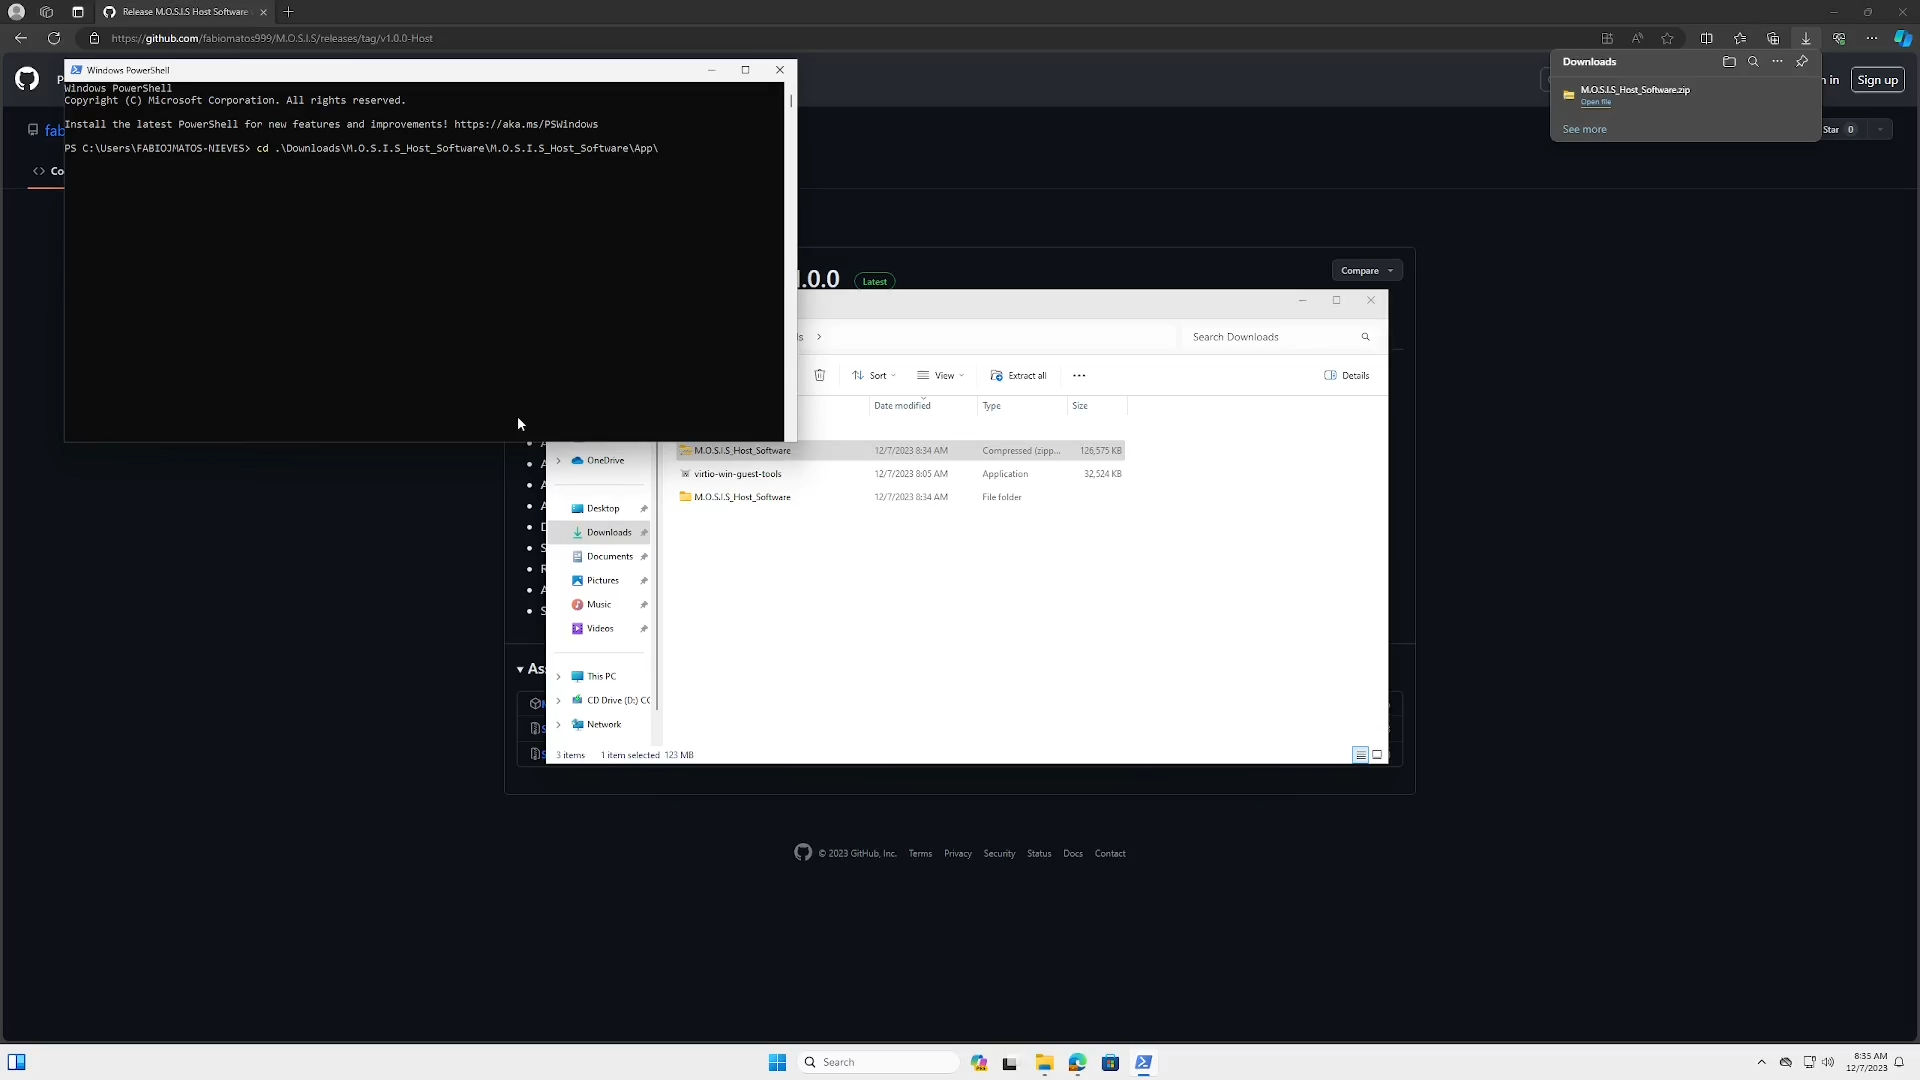
\includegraphics[width=\textwidth]{Figures/Windows-cd-Into-Host-Software.png}
		      \end{figure}
		\item To start the host software and connect to the microscope, first get the IP address of the device by looking at the field above the status bar of the preview screen of the user interface. Then type the following command into the Powershell, substituting ``IPADDRESS'' with the IP address of the microscope.
		      \begin{minted}{ps1}
    .\start_app.ps1 -i IPADDRESS
  \end{minted}
		      \begin{figure}[H]
			      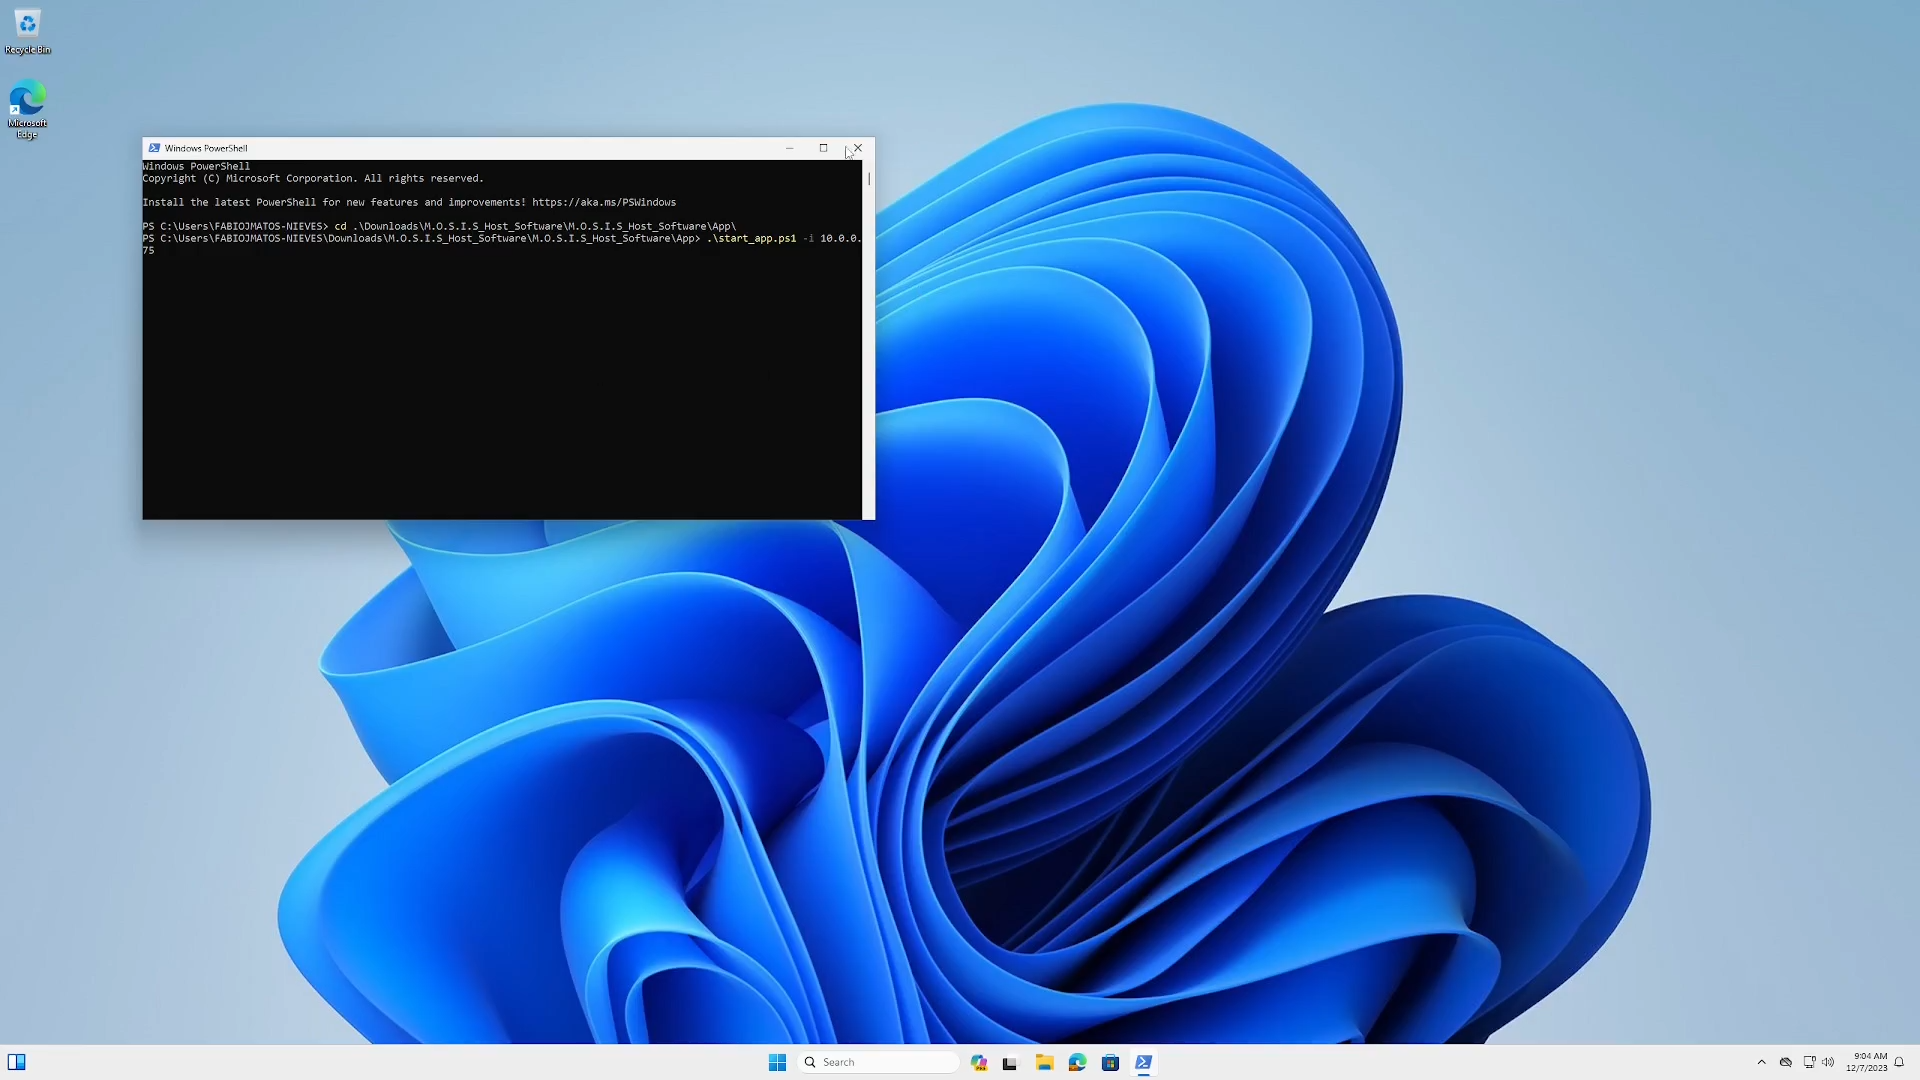
\includegraphics[width=\textwidth]{Figures/Windows-Start-Host-Software-With-IP.png}
		      \end{figure}
		\item If prompted to confirm the ssh key of the microscope, type ``yes'' and press enter.
		      \begin{figure}[H]
			      \includegraphics[width=\textwidth]{Figures/Windows-ssh-authenticity-prompt.png}
		      \end{figure}
		\item You will be prompted to input the password of the M.O.S.I.S microscope Raspberry Pi, type ``pi'' and press enter
		      \begin{figure}[H]
			      \includegraphics[width=\textwidth]{Figures/Windows-pi-password-prompt.png}
		      \end{figure}
		\item You should see output on the screen indicating which files are being transferred from the microscope to the host computer, wait until a web browser tab opens with the host software.
	\end{enumerate}
	\subsection{Linux}
	\item Open a terminal
	\begin{figure}[H]
		\includegraphics[width=\textwidth]{Figures/Linux-Open-terminal.png}
	\end{figure}
	\item Change directory to where the host software was extracted
	\begin{minted}{bash}
                        cd Downloads/M.O.S.I.S_Host_Software/App
                      \end{minted}
	\begin{figure}[H]
		\includegraphics[width=\textwidth]{Figures/Linux-cd-Host-Software.png}
	\end{figure}
	\item To start the host software and connect to the microscope, first get the IP address of the device by looking at the field above the status bar of the preview screen of the user interface. Then type the following command into the Powershell, substituting ``IPADDRESS'' with the IP address of the microscope.

	\begin{minted}{bash}
                       ./start_app.bash -i IPADDRESS
                      \end{minted}
	\begin{figure}[H]
		\includegraphics[width=\textwidth]{Figures/Linux-Start-Host-Software-With-IP.png}
	\end{figure}
	\item If prompted to confirm the ssh key of the microscope, type ``yes'' and press enter.
	\begin{figure}[H]
		\includegraphics[width=\textwidth]{Figures/Linux-SSH-Prompt.png}
	\end{figure}
	\item You will be prompted to input the password of the M.O.S.I.S microscope Raspberry Pi, type ``pi'' and press enter
	\begin{figure}[H]
		\includegraphics[width=\textwidth]{Figures/Linux-Pi-Password.png}
	\end{figure}
	\item You should see output on the screen indicating which files are being transferred from the microscope to the host computer, wait until a web browser tab opens with the host software.
	\begin{figure}[H]
		\includegraphics[width=\textwidth]{Figures/Linux-Transfer-Files.png}
	\end{figure}
	\section{Usage}
	\subsection{Viewing All Captured Media}
	\subsection{Viewing A Specific Captured Media}
	\subsection{Search}
	\subsubsection{ID}
	\subsubsection{Shot Type}
	\subsubsection{Illumination Type}
	\subsubsection{Date}
	\subsection{Study Profile Creation}
	\subsection{Study Profile Upload}
	\section{Backup Raspberry Pi Media}
	\section{Backup Raspberry Pi SD Card}
\end{center}
\end{document}